% \documentclass[final, double]{ua-thesis}
\documentclass[final, double]{ua-thesis}

%\linenumbers
\usepackage{natbib}
\usepackage{setspace}
% \usepackage[sectionbib]{chapterbib}

\BeforeBeginEnvironment{tabular}{\begin{center}\footnotesize}
\AfterEndEnvironment{tabular}{\end{center}}


\director{Connie A. Woodhouse}
\author{Steven B. Malevich}
\title{Cool-Season Moisture Delivery and Multi-Basin Streamflow Anomalies in the Western United States}
\date{2017}
\copyrightholder{Steven B. Malevich 2017}

\begin{document}

\maketitle

\chapter*{Acknowledgments}

This dissertation would not be possible without the immense support I received from my major advisor, Dr. Connie Woodhouse. I am grateful to have the opportunity to work with her. Thanks to my minor advisor Dr. Chris Castro for his patient and careful instruction. I would like to thank my committee members for their time and guidance: Dr. Joellen Russell, and Dr. Kevin Anchukaitis.

I would also like to thank Dr. Liz Ritchie and Dr. Stephen Jackson for their support and constructive feedback. Thanks to Dr. Dave Meko, Dr. Clayton Morrison, Dr. Larry Winter, Dr. Kiyomi Morino, Dr. Katie Hirschboeck, and Dr. Andrew Comrie. Thanks to all the faculty and especially the staff in The University of Arizona Department of Geosciences and the Laboratory of Tree-Ring Research. Thanks to the members of my cohort and lab who have provided continuous support despite suffering through countless preliminary talks, drafts, and discussions. An allocation of computer time from the UA Research Computing High Performance Computing (HPC) and High Throughput Computing (HTC) at the University of Arizona is gratefully acknowledged. Finally, I want to thank the reader who takes the time to look through this dissertation.

This research was supported by the US Bureau of Reclamation WaterSmart program (Agreement \# R11 AP 81 457). I am also thankful for support from the Galileo Circle Scholarship. 

\chapter*{Dedication}
This dissertation is dedicated to my wise and beautiful wife.

\tableofcontents
\listoffigures
\listoftables

\begin{abstract}
Widespread droughts can have a significant impact on western United States streamflow, but the causes of these events are not fully understood. This dissertation examines streamflow from multiple western US basins and establishes the robust, leading modes of variability in interannual streamflow throughout the past century. I show that approximately 50\% of this variability is associated with spatially widespread streamflow anomalies that are statistically independent from streamflow’s response to the El Ni\~{n}o-Southern Oscillation (ENSO). The ENSO-teleconnection accounts for approximately 25\% of the interannual variability in streamflow, across this network. These atmospheric circulation anomalies associated with the most spatially widespread variability are associated with the Aleutian low and the persistent coastal atmospheric ridge in the Pacific Northwest. I use a watershed segmentation algorithm to explicitly track the position and intensity of these features and compare their variability to the multi-basin streamflow variability. Results show that latitudinal shifts in the coastal atmospheric ridge are more strongly associated with streamflow’s north-south dipole response to ENSO variability while more spatially widespread anomalies in streamflow most strongly relate to seasonal changes in the coastal ridge intensity. This likely reflects persistent coastal ridge blocking of cool-season precipitation into western US river basins. I utilize the 35 model runs of the Community Earth System Model Large Ensemble (CESMLE) to determine whether the model ensemble simulates the anomalously strong coastal ridges and extreme widespread wintertime precipitation anomalies found in the observation record. Though there is considerable bias in the CESMLE, the CESMLE runs simulate extremely widespread dry precipitation anomalies with a frequency of approximately one extreme event per century during the historical simulations (1920 - 2005). These extremely widespread dry events correspond significantly with anomalously intense coastal atmospheric ridges. The results from these three papers connect widespread interannual streamflow anomalies in the western US - and especially extremely widespread streamflow droughts - with semi-permanent atmospheric ridge anomalies near the coastal Pacific Northwest. This is important to western US water managers because these widespread events appear to have been a robust feature of the past century. The semi-permanent atmospheric features associated with these widespread dry streamflow anomalies are projected to change position significantly in the next century as a response to global climate change. This may change widespread streamflow anomaly characteristic in the western US, though my results do not show evidence of these changes within the instrument record of last century.
\end{abstract}

\chapter{Introduction}

\section{The importance of western United States streamflow}

Rivers are a vital resource to the sustainability of both environmental and human systems in the western United States (US). The growth of policy and infrastructure for river water management over the last century has had a dramatic impact on human development. In the West, 75 - 80\% of water resources are diverted for use in agriculture (National Research Council 2007). Much of this water is drawn from large rivers such as California's Sacramento River basin, which irrigates over 2 million acres of agricultural land and is the primary source for freshwater flow into San Francisco Bay \citep{domagalski_national_1994}. In the Pacific Northwest, 60 - 70\% of energy supplies are produced by hydroelectric dams \citep{u.s._bureau_of_reclamation_secure_2016}. Within this subregion, several organizations operate a complex network of dams. The US Bureau of Reclamation, for instance, has an active capacity of approximately 22 km$^3$ of water distributed across 50 dams within this system \citep{u.s._bureau_of_reclamation_secure_2016}. In the interior and southwest US, the Colorado River and its tributaries contribute to the municipal water needs of a growing population that is nearing 50 million people in California, Colorado, Nevada, New Mexico, Utah, Wyoming, and Arizona \citep{u.s._bureau_of_reclamation_secure_2016}. Rapid urban population growth in the western US has underlined a shift where water allocated for agriculture is increasingly used to meet the increasing water demand from growing urban populations in multiple watersheds \citep{national_research_council_colorado_2007}. Water managers in Phoenix, Arizona, for example, have seen water demand for agricultural use decrease by roughly 42\% from 1985 to 2006 \citep{arizona_department_of_water_resources_phoenix_2011}. During the same period of time, water demand for municipal use nearly doubled, accounting for half of the total water demand in 2006 \citep{arizona_department_of_water_resources_phoenix_2011}.

\section{Climate influences and regional air circulation}

Western US streamflow is largely driven by cool-season storms that move moisture from the Pacific Ocean eastward, forming snowpack over the North American Cordillera \citep{rasmusson_atmospheric_1967, klein_specification_1987, hsu_global_1976}. This snowpack melts in the spring, feeding major river basins of the western US. There is a wide range of moisture variability within the region. Local orographic effects can dramatically influence basin drainage and affect which storms are blocked by topography or captured in a river basin \citep[e.g., ][]{changnon_hydroclimatic_1991}.

Western US winter precipitation is modulated by the northern hemisphere jet stream and the equatorial Pacific (e.g. El Ni\~{n}a-Southern Oscillation; ENSO) and North Pacific decadal variability \citep{redmond_surface_1991, dettinger_northsouth_1998, cayan_enso_1999, wise_spatiotemporal_2010}. These sources of variability act through atmospheric Rossby waves in the local mid-latitudes, influencing moisture transport \citep{bjerknes_atmospheric_1969, horel_planetary-scale_1981}. While a hydroclimate response to teleconnections can be simple and linear, as in the north-south seesaw or ``dipole'' response to ENSO variability in the western US \citep{brown_winter_2004}, these phenomena are not strictly independent of one another, leading to complex interactions \citep{frankignoul_stochastic_1977, alexander_surface_1997, newman_enso-forced_2003}. Changes in atmospheric circulation can be caused by non-linear internal dynamics or a combination of teleconnections \citep{feldstein_timescale_2000}. 

During the cool-season, intensified mid-latitude wave trains help guide storm tracks from the Pacific Ocean, influencing the western North American hydroclimate \citep{yarnal_relationships_1986, leathers_pacific/north_1991, redmond_surface_1991}. These influences are often quantified in climate studies using Eulerian methods \citep[e.g., ][]{wallace_teleconnections_1981}, that identify major modes of ocean or atmosphere variability and often define simplified climate indices (such as the Pacific-North American Pattern; PNA) from these established modes or centers of action. However, hydroclimate studies have often focused on the influence of specific, semi-permanent features, such as the Aleutian low and coastal Pacific Northwest ridge. The Aleutian low and the coastal Pacific Northwest (or Rocky Mountain) ridge are semi-permanent air masses that are local components of this mid-latitude wave system and a larger standing atmospheric wave anchored over western North America that form from the joint influence of orography, transient eddies, and diabatic heating \citep{charney_numerical_1949, hoskins_steady_1981}. In streamflow and precipitation studies in the western US, these semi-permanent air masses have been associated with widespread covariability and especially extreme widespread drought events \citep{mcguirk_century_1982, cayan_influence_1989, cook_worst_2014, seager_causes_2014, wise_five_2016}.

\section{Impact of widespread streamflow anomalies in the western United States}

Understanding regional hydroclimate variability and multi-basin covariability in streamflow is especially important as water managers draw water from multiple river basins to meet demand and mitigate the impact of drought. California's urban and agricultural centers, for example, draw water allocations from the Colorado River outside of California, which provides critical water supplies to six other US states and Mexico. Many of the most extreme, spatially widespread streamflow droughts in the West have been associated with persistent coastal ridges along the US Pacific coast. The recent California drought in the first half of the 2010s is a frequently cited example of the coastal ridge influence. A perhaps more infamous example is from the 1976 - 1977 winter wherein an unusually intense coastal atmospheric ridge led to one of the driest winters on record \citep[e.g., ][]{seager_causes_2014}. The 1976 - 1977 event had significant economic and political impact on the western US.

In California prior to the 1977 event, there were no policy requirements for local government water management organizations to conduct long-term resource planning \citep{california_department_of_water_resources_2015_2016}. California passed the Urban Water Management Planning Act, which passed after the 1977 drought, was a response to the drought's widespread and severe impacts. For instance, the Marin Municipal Water District faced rapidly depleting supplies despite having successfully implemented water rationing plans. Through coordination with the California Department of Water Resources and other water districts, a temporary 10 km pipeline was constructed to carry water from the State Water Project in the East Bay to Marin County \citep{california_department_of_water_resources_2015_2016}. A forward by the director of the Department of Water Resources, Ronald B. Robie, in a state drought report from February, 1977 \citep{california_department_of_water_resources_california_1977} hints at the tone and impact of the event:
\begin{quote}
\ldots Already significant rationing is under way in many parts of the State, and substantial deficiencies have been imposed by federal, state, and local water projects. Most hard hit are agricultural users. Many actions have been taken by the State in conjunction with federal, state, and local agencies to alleviate emergency situation\ldots

Much more needs to be done. Every individual in our State and every agency supplying urban water must take actions immediately to \underline{substantially reduce} \underline{water use} [original emphasis], not only to meet current needs but to ensure the largest possible carryover supplies for next year – which may also be dry.

Managing water resources during the current drought will place substantial obligations on and require sacrifices by individuals and government alike.

As Governor Edmund G. Brown Jr. said, in his message to the Legislature on January 6, 1977, \underline{``We are going to have to learn to share, north and south, all} \underline{of us together. It is the only way we can solve this problem.''} [original emphasis]
\end{quote}

The economic consequences to California agriculture and livestock of the 1976 - 1977 winter drought were substantial, with estimated losses in 1976 at \$500 million (now \$2.1 billion, adjusted) \citep{us_government_accountability_office_california_1977}. Drought-related losses to agriculture, energy, recreation, and forestry in 1977 were estimated at \$1.8 billion (\$7.1 billion, adjusted) \citep{california_department_of_water_resources_1976_1977}.

\section{Climate change Projections and western US streamflow}

Potential climate change impacts add a layer of complexity to existing water supply problems and are of concern to western US water management and stakeholders \citep{dettinger_western_2015}. Potential impacts include increased demand for water, increased pressure on basin ecosystems, and increased stress from extreme events such as heat waves, flooding, and drought \citep[e.g., ][]{mote_declining_2005, brekke_addressing_2011, garfin_assessment_2013}. Recent research points out that uncertainty in projected changes in North Pacific atmospheric circulation, especially in the eastern North Pacific, strongly influences precipitation projections in parts of the western US \citep[e.g., ][]{langenbrunner_patterns_2015, choi_uncertainty_2016}. A recent US Bureau of Reclamation SECURE Water Act report \citep{u.s._bureau_of_reclamation_secure_2016} highlights key observations and projections important to western US water management. These include 1) temperature increases and decreases in snowpack with changes in the seasonality and volume of spring runoff; 2) increased and basin-dependent impact from extreme precipitation events relating to flooding and drought; 3) projections of increased winter runoff in Pacific coastal river basins but little-to-no trend for runoff in the Southern Rockies and southwest US; 4) projections of a dramatic decline in summer runoff in the southern half of the western US; and, 5) projections of an increase in annual precipitation in the northern western US and decreases in the south western US.

\section{General circulation models and uncertainty in climate change projections}

There are considerable uncertainties in western US climate projections and impact assessments. A 2016 US Bureau of Reclamation climate risk assessment has underlined key uncertainties in 1) the global climate models (GCMs) used for projections, 2) downscaling of climate projections to the western US, and 3) hydrologic modeling of the west US within these projections \citep{us_bureau_of_reclamation_west-wide_2016}. Uncertainty in GCMs ensembles deals with the structure of these models and the influence from internal climate variability, which is of particular interest for my research, here. Climate systems have a chaotic evolution \citep{lorenz_deterministic_1963}, where small changes in the initial conditions can lead to a significantly different outcome in the system and this different outcome is due to internal variability rather than model error or a misrepresentation of the physical climate processes \citep{deser_uncertainty_2012, deser_communication_2012, knutti_climate_2013, tebaldi_mapping_2011}. This internal variability can have an important impact on western US climate systems, causing changes of practical significance even in the absense of an external perturbation. Yet, many GCM ensembles used in climate assessments do not explicitly quantify this internal variability, instead relying on ``ensembles of opportunity'' \citep{murphy_quantification_2004, tebaldi_use_2007, knutti_challenges_2009}. Some GCM experiments, like the Community Earth System Model Large Ensemble (CESMLE) have attempted to estimate internal variability with much larger ensembles of the same model run under similar forcing and initializing conditions \citep{kay_community_2014}. This large ensemble approach may be a useful tool to incorporate into climate impact assessments \citep{us_bureau_of_reclamation_west-wide_2016}, but more work is needed to understand its strengths and limitations.

\section{Summary}

Years with widespread streamflow anomalies can have a significant impact on the western US. These events are often associated with Pacific ocean and internal atmospheric variability, though relatively few studies have explicitly examined the link between annual multi-basin streamflow anomalies and climate. Climate change is also likely to compound existing water supply problems in the western US, though there are outstanding questions about how best to quantify uncertainty and internal climate variability within the climate models used for climate change projections and climate impact assessments.

\chapter{Present Study}

This dissertation examines climate variability that has directly caused major widespread or multi-basin interannual streamflow anomalies in the western US. I examine how these widespread anomalies are linked specifically to the Aleutian low and the semi-permanent coastal Pacific Northwest ridge. I also examine how well extreme and widespread wintertime drought events are represented in the CESMLE. The dissertation is organized into three scientific papers found in the Appendix. The first paper, \textit{Pacific SSTs, mid-latitude atmospheric circulation and widespread interannual anomalies in Western US streamflow} is currently in revision for \textit{Geophysical Research Letters}. The second paper, \textit{The importance of coastal Pacific ridge and Aleutian low position and intensity for widespread interannual anomalies in western US streamflow}, is prepared for submission to the \textit{Journal of Climate}, and the final paper, \textit{Extreme widespread Western US precipitation anomalies and wintertime Pacific coast atmospheric ridges in the CESM Large Ensemble historical simulations} is prepared for submission to \textit{Geophysical Research Letters}. At present, I am the leading author for each of these papers with my major advisor Dr. Connie Woodhouse as coauthor.

This chapter is a brief review of the goals, methods, and conclusions for each of these papers.

\section{Pacific SSTs, mid-latitude atmospheric circulation and widespread interannual anomalies in Western US streamflow}

My first paper uses the 2009 update of the US Geological Survey Hydroclimate Data Network streamflow gages \citep{lins_usgs_2012} to establish whether widespread interannual streamflow anomalies in the western US can be statistically separated from Pacific SST, and specifically ENSO teleconnections. I use western US streamflow data from 169 instrument river gages extending back to 1925. The study approaches the problem with a principal components analysis (PCA) framework \citep{wilks_statistical_2006}.

I show that widespread interannual streamflow anomalies are a temporally consistent and robust feature of the past century by examining different subsets of gages over different periods of time. My main analysis includes comparing the leading streamflow principal components with sea-surface temperature (SST) and atmospheric circulation (500 mb geopotential heights) from NOAA Extended Reconstructed SST V3b fields \citep{smith_improvements_2008} and the Twentieth Century Reanalysis Version 2 \citep{compo_twentieth_2011}, respectively.

The results suggest that interannual streamflow in the western US has two leading modes of variability which associate with 1) cool-season wave trains in the North Pacific, and specifically air pressure anomalies related to the Aleutian low and coastal North Pacific ridges; and 2) the classic, linear, dipole response to ENSO-teleconnections. This first mode, relating to cool-season atmosphere circulation in the North Pacific accounts for approximately 50\% of interannual streamflow variability, while the mode relating to ENSO-teleconnections accounts for roughly 25\% of variability. The first mode of streamflow variability is associated with the most widespread streamflow anomalies akin to that experienced in the extremely dry 1976 - 1977 winter.

\section{The importance of coastal Pacific ridge and Aleutian low position and intensity for widespread interannual anomalies in western US streamflow}

This second paper examines how the seasonal position and intensity of the semi-permanent Aleutian low and Pacific coastal ridge, both of which have been associated with widespread streamflow anomalies. One novelty of this study is the use of a segmentation algorithm to isolate the coastal ridge and Aleutian low and explicitly track changes in their position and intensity through time.

Unlike the previous paper, here I focus on a few select streamflow gages that are from physically independent basins, and have some significance to western US water management. Specifically, I look at the ``Colorado River at Lees Ferry, AZ'', ``Columbia River at The Dalles, OR'', ``Missouri River at Toston, MT'', ``Sacramento Four Rivers Index'', and the ``South Platte River at South Platte, CO''. These streamflow series extend from 1930 - 2006.

Results from this study indicate that widespread interannual streamflow variability is more strongly associated with changes in the coastal ridge intensity, while the Aleutian low also has significant relationships with streamflow, these are not as strong and are largely isolated to the Northern US Rockies and the Pacific Northwest. The analysis shows a significant relationship between the ridge latitudinal position and streamflow's ENSO-teleconnection dipole response.

\section{Extreme widespread Western US precipitation anomalies and wintertime Pacific coast atmospheric ridges in the CESM Large Ensemble historical simulations}

The goal of the final paper is to examine whether the 35 model runs in the CESMLE historical period (1920 - 2005) are able to simulate 1976-1977-like events consisting of extreme widespread, wintertime, low precipitation anomalies across the western US. The study also examines whether these events are significantly associated with unusually intense wintertime coastal Pacific Northwest ridges, which was a outstanding characteristic of the 1976 - 1977 drought.

I used the same segmentation algorithm established in the second paper to track ridge behavior in the 35 CESMLE runs. I searched for simple bias in the model by comparing the CESMLE mean with reanalysis products for atmospheric circulation (geopotential height at 500 mb) from the ERA-Interim \citep{dee_era-interim_2011} and the NOAA-CIRES Twentieth Century Reanalysis Version 2c \citep{compo_twentieth_2011}, and precipitation from the Global Precipitation Climatology Project v2.3 \citep{adler_version-2_2003} and the Global Precipitation Climatology Center version 7 \citep{schneider_gpcc_2015}.

Results show that the CESMLE mean is bias towards more intense ridges and wet anomalies in the western US. Additionally, the CESMLE poorly simulates subregional precipitation features in the western US. Several extreme widespread events were found within 35 CESMLE runs, which appears to produce approximately one extreme widespread event every century during the simulated historical period (1920 - 2005). These events have a very strong and statistically significant association with anomalously intense wintertime coastal ridges.

\bibliographystyle{ametsoc2014}
% \bibliography{references}

\begin{thebibliography}{}
\providecommand{\natexlab}[1]{#1}
\providecommand{\url}[1]{\texttt{#1}}
\renewcommand{\UrlFont}{\rmfamily}
\providecommand{\urlprefix}{URL }
\expandafter\ifx\csname urlstyle\endcsname\relax
  \providecommand{\doi}[1]{doi:\discretionary{}{}{}#1}\else
  \providecommand{\doi}{doi:\discretionary{}{}{}\begingroup
  \urlstyle{rm}\Url}\fi
\providecommand{\eprint}[2][]{\url{#2}}

\bibitem[{Adler et~al.(2003)}]{adler_version-2_2003}
Adler, R.~F., and Coauthors, 2003: The {Version}-2 {Global} {Precipitation}
  {Climatology} {Project} ({GPCP}) {Monthly} {Precipitation} {Analysis}
  (1979–{Present}). \textit{J. Hydrometeor.}, \textbf{4~(6)}, 1147--1167,
  \doi{10.1175/1525-7541(2003)004<1147:TVGPCP>2.0.CO;2}.

\bibitem[{Alexander and Scott(1997)Alexander, and
  Scott}]{alexander_surface_1997}
Alexander, M.~A., and J.~D. Scott, 1997: Surface {Flux} {Variability} over the
  {North} {Pacific} and {North} {Atlantic} {Oceans}. \textit{J. Climate},
  \textbf{10~(11)}, 2963--2978,
  \doi{10.1175/1520-0442(1997)010<2963:SFVOTN>2.0.CO;2},

\bibitem[{{Arizona Department of Water
  Resources}(2011)}]{arizona_department_of_water_resources_phoenix_2011}
{Arizona Department of Water Resources}, 2011: Phoenix {Active} {Management}
  {Area}, {Water} {Demand} and {Supply} {Assessment}: 1985 - 2025. Tech. rep.,
  State of Arizona, Department of Water Resources.
  \urlprefix\url{http://www.azwater.gov/AzDWR/WaterManagement/Assessments/documents/PhxAMA_AssessmentSummarySheet.pdf}.

\bibitem[{Bjerknes(1969)}]{bjerknes_atmospheric_1969}
Bjerknes, J., 1969: Atmospheric teleconnections from the equatorial {Pacific}.
  \textit{Monthly Weather Review}, \textbf{97~(3)}, 163--172,
  \doi{10.1175/1520-0493(1969)097<0163:ATFTEP>2.3.CO;2},

\bibitem[{Brekke(2011)}]{brekke_addressing_2011}
Brekke, L.~D., 2011: Addressing {Climate} {Change} in {Long}-{Term} {Water}
  {Resources} {Planning} and {Management}: {User} {Needs} for {Improving}
  {Tools} and {Information}. Technical {Report} CWTS 10-02, U.S. Army Corps of
  Engineers, U.S. Bureau of Reclamation, 160 pp.
  \urlprefix\url{http://www.usbr.gov/climate/userneeds/index.html}.

\bibitem[{Brown and Comrie(2004)Brown, and Comrie}]{brown_winter_2004}
Brown, D.~P., and A.~C. Comrie, 2004: A winter precipitation 'dipole' in the
  western {United} {States} associated with multidecadal {ENSO} variability.
  \textit{Geophysical research letters.}, \textbf{31~(9)}, L09\,203.

\bibitem[{{California Department of Water
  Resources}(1977)}]{california_department_of_water_resources_california_1977}
{California Department of Water Resources}, 1977: The {California} drought -
  1977: {An} {Update}. Tech. rep., 161 pp.
  
\bibitem[{{California Department of Water
  Resources}(1978)}]{california_department_of_water_resources_1976_1977}
{California Department of Water
  Resources}, The 1976 - 1977 {California} {Drought}: {A} {Review}. 239 pp.

\bibitem[{{California Department of Water
  Resources}(2016)}]{california_department_of_water_resources_2015_2016}
{California Department of Water Resources}, 2016: 2015 {Urban} {Water}
  {Management} {Plans}: {Guidebook} for {Urban} {Water} {Suppliers}. Tech.
  rep., 191 pp.
  \urlprefix\url{http://www.water.ca.gov/urbanwatermanagement/docs/2015/UWMP_Guidebook_Mar_2016_FINAL.pdf}.

\bibitem[{Cayan and Peterson(1989)Cayan, and Peterson}]{cayan_influence_1989}
Cayan, D.~R., and D.~H. Peterson, 1989: The {Influence} of {North} {Pacific}
  {Atmospheric} {Circulation} on {Streamflow} in the {West}. \textit{Aspects of
  {Climate} {Variability} in the {Pacific} and the {Western} {Americas}}, D.~H.
  Peterson, Ed., American Geophysical Union, Washington, D. C., 375--397,
  doi: 10.1029/GM055p0375.

\bibitem[{Cayan et~al.(1999)Cayan, Redmond,, and Riddle}]{cayan_enso_1999}
Cayan, D.~R., K.~T. Redmond, and L.~G. Riddle, 1999: {ENSO} and {Hydrologic}
  {Extremes} in the {Western} {United} {States}. \textit{J. Clim.},
  \textbf{12~(9)}, 2881--2893,
  \doi{10.1175/1520-0442(1999)012<2881:EAHEIT>2.0.CO;2},

\bibitem[{Changnon et~al.(1991)Changnon, McKee,, and
  Doesken}]{changnon_hydroclimatic_1991}
Changnon, D., T.~B. McKee, and N.~J. Doesken, 1991: Hydroclimatic variability
  in the {Rocky} {Mountains}. \textit{J Am Water Resources Assoc},
  \textbf{27~(5)}, 733--743, \doi{10.1111/j.1752-1688.1991.tb01471.x}.

\bibitem[{Charney and Eliassen(1949)Charney, and
  Eliassen}]{charney_numerical_1949}
Charney, J.~G., and A.~Eliassen, 1949: A {Numerical} {Method} for {Predicting}
  the {Perturbations} of the {Middle} {Latitude} {Westerlies}. \textit{Tellus},
  \textbf{1~(2)}, 38--54, \doi{10.1111/j.2153-3490.1949.tb01258.x}.

\bibitem[{Choi et~al.(2016)Choi, Lu, Son, Frierson,, and
  Yoon}]{choi_uncertainty_2016}
Choi, J., J.~Lu, S.-W. Son, D.~M.~W. Frierson, and J.-H. Yoon, 2016:
  Uncertainty in future projections of the {North} {Pacific} subtropical high
  and its implication for {California} winter precipitation change. \textit{J.
  Geophys. Res. Atmos.}, \textbf{121~(2)}, 2015JD023\,858,
  \doi{10.1002/2015JD023858},

\bibitem[{Clark(1999)}]{clark_brief_1999}
Clark, A.~H., 1999: A brief discussion of {Klamath} basin geology and geography
  related to water resources. \textit{A {River} {Never} the {Same} : {A}
  {History} of {Water} in the {Klamath} {Basin}}, L.~W. Powers, Ed., Cambridge
  Univ. Press, Klamath Falls, OR.

\bibitem[{Compo et~al.(2011)}]{compo_twentieth_2011}
Compo, G.~P., and Coauthors, 2011: The {Twentieth} {Century} {Reanalysis}
  {Project}. \textit{Q.J.R. Meteorol. Soc.}, \textbf{137~(654)}, 1--28,
  \doi{10.1002/qj.776},

\bibitem[{Cook et~al.(2014)Cook, Seager,, and Smerdon}]{cook_worst_2014}
Cook, B.~I., R.~Seager, and J.~E. Smerdon, 2014: The worst {North} {American}
  drought year of the last millennium: 1934. \textit{Geophys. Res. Lett.},
  \textbf{41~(20)}, 7298--7305, \doi{10.1002/2014GL061661}.

\bibitem[{Dee et~al.(2011)}]{dee_era-interim_2011}
Dee, D.~P., and Coauthors, 2011: The {ERA}-{Interim} reanalysis: configuration
  and performance of the data assimilation system. \textit{Q.J.R. Meteorol.
  Soc.}, \textbf{137~(656)}, 553--597, \doi{10.1002/qj.828},

\bibitem[{Deser et~al.(2012{\natexlab{a}})Deser, Knutti, Solomon,, and
  Phillips}]{deser_communication_2012}
Deser, C., R.~Knutti, S.~Solomon, and A.~S. Phillips, 2012{\natexlab{a}}:
  Communication of the role of natural variability in future {North} {American}
  climate. \textit{Nature Clim. Change}, \textbf{2~(11)}, 775--779,
  \doi{10.1038/nclimate1562},

\bibitem[{Deser et~al.(2012{\natexlab{b}})Deser, Phillips, Bourdette,, and
  Teng}]{deser_uncertainty_2012}
Deser, C., A.~Phillips, V.~Bourdette, and H.~Teng, 2012{\natexlab{b}}:
  Uncertainty in climate change projections: the role of internal variability.
  \textit{Climate Dynamics}, \textbf{38~(3-4)}, 527--546,
  \doi{10.1007/s00382-010-0977-x}.

\bibitem[{Dettinger et~al.(2015)Dettinger, Udall,, and
  Georgakakos}]{dettinger_western_2015}
Dettinger, M., B.~Udall, and A.~Georgakakos, 2015: Western water and climate
  change. \textit{Ecological Applications}, \textbf{25~(8)}, 2069--2093,
  \doi{10.1890/15-0938.1},

\bibitem[{Dettinger et~al.(1998)Dettinger, Cayan, Diaz,, and
  Meko}]{dettinger_northsouth_1998}
Dettinger, M.~D., D.~R. Cayan, H.~F. Diaz, and D.~M. Meko, 1998:
  North–{South} {Precipitation} {Patterns} in {Western} {North} {America} on
  {Interannual}-to-{Decadal} {Timescales}. \textit{J. Clim.}, \textbf{11~(12)},
  3095--3111, \doi{10.1175/1520-0442(1998)011<3095:NSPPIW>2.0.CO;2},

\bibitem[{Domagalski and Brown(1994)Domagalski, and
  Brown}]{domagalski_national_1994}
Domagalski, J., and L.~Brown, 1994: National {Water}-{Quality} {Assessment}
  {Program}: {The} {Sacramento} {River} {Basin}. Fact {Sheet} 1994-029, U.S.
  Geological Survey.

\bibitem[{Feldstein(2000)}]{feldstein_timescale_2000}
Feldstein, S.~B., 2000: The {Timescale}, {Power} {Spectra}, and {Climate}
  {Noise} {Properties} of {Teleconnection} {Patterns}. \textit{J. Climate},
  \textbf{13~(24)}, 4430--4440,
  \doi{10.1175/1520-0442(2000)013<4430:TTPSAC>2.0.CO;2},

\bibitem[{Frankignoul and Hasselmann(1977)Frankignoul, and
  Hasselmann}]{frankignoul_stochastic_1977}
Frankignoul, C., and K.~Hasselmann, 1977: Stochastic climate models, {Part}
  {II} {Application} to sea-surface temperature anomalies and thermocline
  variability. \textit{Tellus}, \textbf{29~(4)}, 289--305,
  \doi{10.1111/j.2153-3490.1977.tb00740.x},

\bibitem[{Garfin et~al.(2013)Garfin, Jardine, Merideth, Black,, and
  LeRoy}]{garfin_assessment_2013}
Garfin, G., A.~Jardine, R.~Merideth, M.~Black, and S.~LeRoy, 2013:
  \textit{Assessment of {Climate} {Change} in the {Southwest} {United}
  {States}: {A} {Report} {Prepared} for the {National} {Climate} {Assessment}}.
  Island Press., Washington, D.C.,
  \urlprefix\url{http://www.swcarr.arizona.edu/}.

\bibitem[{Horel and Wallace(1981)Horel, and
  Wallace}]{horel_planetary-scale_1981}
Horel, J.~D., and J.~M. Wallace, 1981: Planetary-{Scale} {Atmospheric}
  {Phenomena} {Associated} with the {Southern} {Oscillation}. \textit{Monthly
  Weather Review}, \textbf{109~(4)}, 813--829,
  \doi{10.1175/1520-0493(1981)109<0813:PSAPAW>2.0.CO;2}.

\bibitem[{Hoskins and Karoly(1981)Hoskins, and Karoly}]{hoskins_steady_1981}
Hoskins, B.~J., and D.~J. Karoly, 1981: The {Steady} {Linear} {Response} of a
  {Spherical} {Atmosphere} to {Thermal} and {Orographic} {Forcing}. \textit{J.
  Atmos. Sci.}, \textbf{38~(6)}, 1179--1196,
  \doi{10.1175/1520-0469(1981)038<1179:TSLROA>2.0.CO;2},

\bibitem[{Hsu and Wallace(1976)Hsu, and Wallace}]{hsu_global_1976}
Hsu, C.-P.~F., and J.~M. Wallace, 1976: The {Global} {Distribution} of the
  {Annual} and {Semiannual} {Cycles} in {Precipitation}. \textit{Mon. Wea.
  Rev.}, \textbf{104~(9)}, 1093--1101,
  \doi{10.1175/1520-0493(1976)104<1093:TGDOTA>2.0.CO;2},

\bibitem[{Kay et~al.(2014)}]{kay_community_2014}
Kay, J.~E., and Coauthors, 2014: The {Community} {Earth} {System} {Model}
  ({CESM}) {Large} {Ensemble} {Project}: {A} {Community} {Resource} for
  {Studying} {Climate} {Change} in the {Presence} of {Internal} {Climate}
  {Variability}. \textit{Bull. Amer. Meteor. Soc.}, \textbf{96~(8)},
  1333--1349, \doi{10.1175/BAMS-D-13-00255.1},

\bibitem[{Klein and Bloom(1987)Klein, and Bloom}]{klein_specification_1987}
Klein, W.~H., and H.~J. Bloom, 1987: Specification of {Monthly} {Precipitation}
  over the {United} {States} from the {Surrounding} 700 mb {Height} {Field}.
  \textit{Mon. Wea. Rev.}, \textbf{115~(9)}, 2118--2132,
  \doi{10.1175/1520-0493(1987)115<2118:SOMPOT>2.0.CO;2},

\bibitem[{Knutti et~al.(2009)Knutti, Furrer, Tebaldi, Cermak,, and
  Meehl}]{knutti_challenges_2009}
Knutti, R., R.~Furrer, C.~Tebaldi, J.~Cermak, and G.~A. Meehl, 2009: Challenges
  in {Combining} {Projections} from {Multiple} {Climate} {Models}. \textit{J.
  Climate}, \textbf{23~(10)}, 2739--2758, \doi{10.1175/2009JCLI3361.1}.

\bibitem[{Knutti et~al.(2013)Knutti, Masson,, and
  Gettelman}]{knutti_climate_2013}
Knutti, R., D.~Masson, and A.~Gettelman, 2013: Climate model genealogy:
  {Generation} {CMIP}5 and how we got there. \textit{Geophys. Res. Lett.},
  \textbf{40~(6)}, 1194--1199, \doi{10.1002/grl.50256},

\bibitem[{Langenbrunner et~al.(2015)Langenbrunner, Neelin, Lintner,, and
  Anderson}]{langenbrunner_patterns_2015}
Langenbrunner, B., J.~D. Neelin, B.~R. Lintner, and B.~T. Anderson, 2015:
  Patterns of {Precipitation} {Change} and {Climatological} {Uncertainty} among
  {CMIP}5 {Models}, with a {Focus} on the {Midlatitude} {Pacific} {Storm}
  {Track}. \textit{J. Climate}, \textbf{28~(19)}, 7857--7872,
  \doi{10.1175/JCLI-D-14-00800.1},

\bibitem[{Leathers et~al.(1991)Leathers, Yarnal,, and
  Palecki}]{leathers_pacific/north_1991}
Leathers, D.~J., B.~Yarnal, and M.~A. Palecki, 1991: The {Pacific}/{North}
  {American} {Teleconnection} {Pattern} and {United} {States} {Climate}. {Part}
  {I}: {Regional} {Temperature} and {Precipitation} {Associations}.
  \textit{Journal of Climate}, \textbf{4~(5)}, 517--528,
  \doi{10.1175/1520-0442(1991)004<0517:TPATPA>2.0.CO;2}.

\bibitem[{Levy(2003)}]{levy_turbulence_2003}
Levy, S., 2003: Turbulence in the {Klamath} {River} {Basin}.
  \textit{BioScience}, \textbf{53~(4)}, 315--320,

\bibitem[{Lins(2012)}]{lins_usgs_2012}
Lins, H.~F., 2012: {USGS} {Hydro}-{Climatic} {Data} {Network} 2009
  ({HCDN}-2009). Fact {Sheet} 3047, U.S. Geological Survey, 4 pp.
  \urlprefix\url{http://pubs.usgs.gov/fs/2012/3047/}.

\bibitem[{Lorenz(1963)}]{lorenz_deterministic_1963}
Lorenz, E.~N., 1963: Deterministic {Nonperiodic} {Flow}. \textit{J. Atmos.
  Sci.}, \textbf{20~(2)}, 130--141,
  \doi{10.1175/1520-0469(1963)020<0130:DNF>2.0.CO;2},

\bibitem[{McGuirk(1982)}]{mcguirk_century_1982}
McGuirk, J.~P., 1982: A century of precipitation variability along the pacific
  coast of {North} {America} and its impact. \textit{Climatic Change},
  \textbf{4~(1)}, 41, \doi{10.1007/BF02423312},

\bibitem[{Mote et~al.(2005)Mote, Hamlet, Clark,, and
  Lettenmaier}]{mote_declining_2005}
Mote, P.~W., A.~F. Hamlet, M.~P. Clark, and D.~P. Lettenmaier, 2005: Declining
  mountain snowpack in western {North} {America}. \textit{Bulletin of the
  American Meteorological Society}, \textbf{86~(1)}, 39--49,

\bibitem[{Murphy et~al.(2004)Murphy, Sexton, Barnett, Jones, Webb, Collins,,
  and Stainforth}]{murphy_quantification_2004}
Murphy, J.~M., D.~M.~H. Sexton, D.~N. Barnett, G.~S. Jones, M.~J. Webb,
  M.~Collins, and D.~A. Stainforth, 2004: Quantification of modelling
  uncertainties in a large ensemble of climate change simulations.
  \textit{Nature}, \textbf{430~(7001)}, 768--772, \doi{10.1038/nature02771},

\bibitem[{{National Research
  Council}(2007)}]{national_research_council_colorado_2007}
{National Research Council}, 2007: \textit{Colorado {River} {Basin} water
  management evaluating and adjusting to hydroclimatic variability}. National
  Academies Press, Washington, D.C.,

\bibitem[{Newman et~al.(2003)Newman, Compo,, and
  Alexander}]{newman_enso-forced_2003}
Newman, M., G.~P. Compo, and M.~A. Alexander, 2003: {ENSO}-{Forced}
  {Variability} of the {Pacific} {Decadal} {Oscillation}. \textit{Journal of
  Climate}, \textbf{16~(23)}, 3853--3857,
  \doi{10.1175/1520-0442(2003)016<3853:EVOTPD>2.0.CO;2},

\bibitem[{Rasmusson(1967)}]{rasmusson_atmospheric_1967}
Rasmusson, E.~M., 1967: Atmospheric water vapor transport and the water balance
  of {North} {America}: {Part} {I}. {Characteristics} of the water vapor flux
  field. \textit{Monthly Weather Review}, \textbf{95~(7)}, 403--426,
  \doi{10.1175/1520-0493(1967)095<0403:AWVTAT>2.3.CO;2},

\bibitem[{Redmond and Koch(1991)Redmond, and Koch}]{redmond_surface_1991}
Redmond, K.~T., and R.~W. Koch, 1991: Surface {Climate} and {Streamflow}
  {Variability} in the {Western} {United} {States} and {Their} {Relationship}
  to {Large}-{Scale} {Circulation} {Indices}. \textit{Water Resour. Res.},
  \textbf{27~(9)}, 2381--2399, \doi{10.1029/91WR00690},

\bibitem[{Risley et~al.(2005)Risley, Gannett, Lea,, and
  Roehl~Jr.}]{risley_analysis_2005}
Risley, J.~C., M.~W. Gannett, J.~K. Lea, and E.~A. Roehl~Jr., 2005: An
  {Analysis} of {Statistical} {Methods} for {Seasonal} {Flow} {Forecasting} in
  the {Upper} {Klamath} {River} {Basin} of {Oregon} and {California}.
  Scientific {Investigations} {Report} 2005-5177, U.S. Geological Survey, 43
  pp. \urlprefix\url{http://pubs.usgs.gov/sir/2005/5177/}.

\bibitem[{Schneider et~al.(2015)Schneider, Becker, Finger, Meyer-Christoffer,
  Rudolf,, and Ziese}]{schneider_gpcc_2015}
Schneider, U., A.~Becker, P.~Finger, A.~Meyer-Christoffer, B.~Rudolf, and
  M.~Ziese, 2015: {GPCC} {Full} {Data} {Reanalysis} {Version} 7.0 at 0.5°:
  {Monthly} {Land}-{Surface} {Precipitation} from {Rain}-{Gauges} built on
  {GTS}-based and {Historic} {Data}. Global Precipitation Climatology Centre
  (GPCC) at Deutscher Wetterdienst,
  \doi{10.5676/DWD_GPCC/FD_M_V7_050}.

\bibitem[{Seager et~al.(2014)Seager, Hoerling, Schubert, Wang, Lyon, Kumar,
  Nakamura,, and Henderson}]{seager_causes_2014}
Seager, R., M.~Hoerling, S.~Schubert, H.~Wang, B.~Lyon, A.~Kumar, J.~Nakamura,
  and N.~Henderson, 2014: Causes and {Predictability} of the 2011 to 2014
  {California} {Drought}. Tech. rep., National Oceanic and Atmospheric
  Administration, Washington, D.C.
  \urlprefix\url{http://cpo.noaa.gov/ClimatePrograms/ModelingAnalysisPredictionsandProjections/MAPPTaskForces/DroughtTaskForce1/CaliforniaDrought.aspx}.

\bibitem[{Service(2003)}]{service_combat_2003}
Service, R.~F., 2003: '{Combat} {Biology}' on the {Klamath}. \textit{Science},
  \textbf{300~(5616)}, 36--39,

\bibitem[{Smith et~al.(2008)Smith, Reynolds, Peterson,, and
  Lawrimore}]{smith_improvements_2008}
Smith, T.~M., R.~W. Reynolds, T.~C. Peterson, and J.~Lawrimore, 2008:
  Improvements to {NOAA}’s {Historical} {Merged} {Land}–{Ocean} {Surface}
  {Temperature} {Analysis} (1880–2006). \textit{J. Clim.}, \textbf{21~(10)},
  2283--2296, \doi{10.1175/2007JCLI2100.1},

\bibitem[{Tebaldi et~al.(2011)Tebaldi, Arblaster,, and
  Knutti}]{tebaldi_mapping_2011}
Tebaldi, C., J.~M. Arblaster, and R.~Knutti, 2011: Mapping model agreement on
  future climate projections. \textit{Geophys. Res. Lett.}, \textbf{38~(23)},
  L23\,701, \doi{10.1029/2011GL049863},

\bibitem[{Tebaldi and Knutti(2007)Tebaldi, and Knutti}]{tebaldi_use_2007}
Tebaldi, C., and R.~Knutti, 2007: The use of the multi-model ensemble in
  probabilistic climate projections. \textit{Philosophical Transactions of the
  Royal Society of London A: Mathematical, Physical and Engineering Sciences},
  \textbf{365~(1857)}, 2053--2075, \doi{10.1098/rsta.2007.2076},

% \bibitem[{\textit{Reclamation}(2016a)}]{1reclamation_bureau_of_reclamation_secure_2016}
% {Reclamation (Bureau of Reclamation)} (2016a), {SECURE} {Water} {Act} {Section}
%   9503(c) - {Reclamation} {Climate} {Change} and {Water}. {Prepared} for
%   {United} {States} {Congress}., \textit{Tech. rep.}, Bureau of Reclamation,
%   Policy and Administration, Denver, CO.


\bibitem[{\textit{Reclamation}(2016a)}]{u.s._bureau_of_reclamation_secure_2016}
{Reclamation (Bureau of Reclamation)}, 2016a: {SECURE} {Water} {Act} {Section} 9503(c)
  – {Reclamation} {Climate} {Change} and {Water}. {Prepared} for {United}
  {States} {Congress}. Tech. rep., Bureau of Reclamation, Policy and
  Administration, Denver, CO.

\bibitem[{\textit{Reclamation}(2016b)}]{us_bureau_of_reclamation_west-wide_2016}
{Reclamation (Bureau of Reclamation)}, 2016b: West-{Wide} {Climate} {Risk} {Assessments}:
  {Hydroclimate} {Projections}. Technical {Memorandum} 86-68210-2016-01, U.S.
  Bureau of Reclamation, Denver, Colorado, 154 pp.

\bibitem[{{US Department of the
  Interior}(2010)}]{us_department_of_the_interior_secretary_2010}
{US Department of the Interior}, 2010: Secretary {Salazar}, {Governors}
  {Kulongoski} and {Schwarzenegger} {Announce} {Agreement} on {Klamath} {River}
  {Basin} {Restoration}.
  \urlprefix\url{https://www.doi.gov/news/pressreleases/2010_02_18_release}.

\bibitem[{{US Department of the
  Interior}(2016)}]{us_department_of_the_interior_two_2016}
{US Department of the Interior}, 2016: Two {N}ew {K}lamath {B}asin {A}greements {Carve} out {Path} for {Dam} {Removal} and {Provide} {Key} {Benefits} to {Irrigators}.
  \urlprefix\url{https://www.doi.gov/pressreleases/two-new-klamath-basin-agreements-carve-out-path-dam-removal-and-provide-key-benefits}.

\bibitem[{{US Government Accountability
  Office}(1977)}]{us_government_accountability_office_california_1977}
{US Government Accountability Office}, 1977: California {Drought} of 1976 and
  1977--{Extent}, {Damage}, and {Governmental} {Response}. Report of the
  {Comptroller} {General} of {The} {United} {States} CED-77 137, 108 pp.

\bibitem[{Wallace and Gutzler(1981)Wallace, and
  Gutzler}]{wallace_teleconnections_1981}
Wallace, J.~M., and D.~S. Gutzler, 1981: Teleconnections in the {Geopotential}
  {Height} {Field} during the {Northern} {Hemisphere} {Winter}. \textit{Monthly
  Weather Review}, \textbf{109~(4)}, 784--812,

\bibitem[{Wilks(2006)}]{wilks_statistical_2006}
Wilks, D., 2006: \textit{Statistical {Methods} in the {Atmospheric}
  {Sciences}}. 2nd ed., International geophysics series, Academic Press,
  London, UK.

\bibitem[{Wise(2010)}]{wise_spatiotemporal_2010}
Wise, E.~K., 2010: Spatiotemporal variability of the precipitation dipole
  transition zone in the western {United} {States}. \textit{Geophys. Res.
  Lett.}, \textbf{37~(7)}, L07\,706, \doi{10.1029/2009GL042193}.

\bibitem[{Wise(2016)}]{wise_five_2016}
Wise, E.~K., 2016: Five centuries of {U}.{S}. {West} {Coast} drought:
  {Occurrence}, spatial distribution, and associated atmospheric circulation
  patterns. \textit{Geophys. Res. Lett.}, \textbf{43~(9)}, 2016GL068\,487,
  \doi{10.1002/2016GL068487}.

\bibitem[{Yarnal and Diaz(1986)Yarnal, and Diaz}]{yarnal_relationships_1986}
Yarnal, B., and H.~F. Diaz, 1986: Relationships between extremes of the
  {Southern} oscillation and the winter climate of the {Anglo}-{American}
  {Pacific} {Coast}. \textit{Int. J. Climatol.}, \textbf{6~(2)}, 197--219,
  \doi{10.1002/joc.3370060208}.

\end{thebibliography}


% \begin{thebibliography}{9}
% \section{References}
% \bibliography{references}
% \end{thebibliography}

% \begin{thebibliography}{9}

% \bibitem{A}
% CCIT, Center for Computing \& Information Technology, offers workshops and
% lectures on word processing, graphs and tables, and thesis/dissertation
% formatting.

% \bibitem{B}
% Your advisor and your committee can help; providing assistance on thesis
% formatting, a part of good mentoring.

% \end{thebibliography}


\appendix

\chapter{Pacific SSTs, mid-latitude atmospheric circulation, and widespread interannual anomalies in Western US streamflow}

\section{Abstract}
Widespread droughts can have considerable impact on western United States (US) streamflow, but causes related to moisture delivery processes are not yet fully understood. Here, we examine western US streamflow records to identify robust leading modes of interannual variability and their links to patterns of ocean and atmospheric circulation. The leading mode of streamflow variability, a pattern of west-wide streamflow anomalies, accounts for approximately 50\% of variability and is associated with persistent high pressure anomalies related to ridges off the Pacific North American coast. The second mode of variability accounts for approximately 25\% of variability and is associated with ocean and atmospheric conditions in the Tropical Pacific. Our results suggest that the leading mode of streamflow variability in the western US is more strongly associated with internally-driven mid-latitude atmospheric variability than equatorial Pacific sea surface temperatures.


\section{Introduction}

Droughts affecting streamflow in multiple watersheds can have a profound impact on western United States (US) water supplies. These droughts are often attributed, at least in part, to El Ni\~no-Southern Oscillation (ENSO) variability in the equatorial Pacific \citep{1cayan_enso_1999, 1dettinger_northsouth_1998, 1redmond_surface_1991, 1seager_atmosphere_2014, 1wise_cool-season_2014}. However, many drought events are not directly explained by ENSO alone. Some of the most spatially widespread events in the past century are linked with powerful, cool-season, blocking atmospheric ridges in the mid-latitudes. These features obstruct incoming moisture and are frequently associated with internal atmospheric variability. The unusually strong and widespread droughts in 1977 and 1934 are cited as examples of this \citep [e.g., ][]{1cook_worst_2014, 1hoerling_distinct_2009, 1seager_causes_2014, 1diaz_recent_2015, 1wise_five_2016}. The 2014 California drought is also related to persistent ridging \citep{1cook_worst_2014, 1seager_causes_2015, 1teng_causes_2016, 1wang_probable_2014}. But these examples highlight the often tangled relationship between interacting ocean-atmosphere dynamics in the equatorial and mid-latitude Pacific. For instance, the unusually strong atmospheric ridge during the 2014 drought has been linked with Pacific sea surface temperatures (SST) variability \citep[e.g., ][]{1herring_explaining_2014, 1seager_causes_2015, 1wang_role_2014, 1seager_causes_2014, 1teng_causes_2016, 1wang_probable_2014, 1hartmann_pacific_2015, 1swain_tale_2015}. In the case of the 1934 drought, an unusually intense and persistent atmospheric ridge on the Pacific North American coast was briefly experienced during a longer drought associated with tropical Pacific SSTs \citep{1cook_worst_2014, 1herring_explaining_2014, 1seager_would_2008, 1seager_modeling_2005, 1schubert_cause_2004}. While equatorial Pacific SSTs have been shown to play an important role in triggering western US drought, it is unclear how extensively and consistently the mid-latitude atmosphere circulation \textemdash~independent of tropical Pacific SSTs \textemdash~ can induce widespread drought and hydroclimate variability, particularly in western US streamflow.

Our study approaches this issue with a focus on annual, western US multi-basin streamflow anomalies. Hydroclimate research has largely focused on precipitation, drought-related metrics, or streamflow in specific basins, but rarely on multi-basin streamflow anomalies across the western US. Relative to other hydroclimate variables, the streamflow record has a number of unique and important characteristics. For example, an annual value from a streamflow gage is an integration of hydroclimate processes, spatially, across the extent of a basin or watershed, and temporally, through a full year. As such, it is a measure of the water supply in the basin resulting from these processes. Basin-scale water resources have played a vital role in the human and ecosystem development of the western US. Unlike most other hydroclimate variables, streamflow represents a managed natural resource. In the Pacific Northwest, for example, 60-70\% of energy supplies are produced by hydroelectric dams. Within the Columbia River basin, the US Bureau of Reclamation, alone, manages an active capacity of over 22 km$^3$ of water spread across a network of 50 dams \citep{1reclamation_bureau_of_reclamation_secure_2016}. To the south, a growing population of nearly 50 million people across seven US states have come rely on water allocations from the Colorado River and its tributaries for municipal water needs \citep{1reclamation_bureau_of_reclamation_secure_2016}.

Many of the challenges in Western US water supplies are long-standing issues that are likely to be further confounded by climate change and natural hydroclimate variability that is poorly represented in the instrument record of the last century \citep{1meko_dendrochronology_2012, 1dettinger_western_2015}. An improved understanding of the controls on annual water supply variability is critical for seasonal forecasts and long-term hydroclimate and streamflow projections. The state of ENSO is a widely used as a predictor in seasonal western US forecast models because of its impact on the Western US and seasonal persistence \citep{1liu_atmospheric_2007}. If the mid-latitude ridging patterns that result in widespread streamflow deficits, show consistent preference for one ENSO phase, or some other form of persistent SST variability, this might serve as a basis for improved forecasting and anticipating similar widespread streamflow drought and pluvial events in the future. However, if patterns of widespread streamflow variability are largely free of direct influence from ENSO or other persistent SST patterns, then the droughts and pluvials associated with these streamflow anomalies will generally be difficult, if not impossible to anticipate from seasonal forecasts.

Our main research question is: how consistently are widespread water year (October-September) western US streamflow anomalies associated with mid-latitude atmospheric circulation, without significant and direct influence from equatorial Pacific SSTs? To address this question, we use Principal Components Analysis (PCA) to identify the main patterns or modes of variability in western US streamflow over the last century. The leading principal components (PCs) in streamflow are used to investigate variability in Pacific SSTs and atmospheric circulation corresponding to these main modes of variability. 

\section{Data}

This study used water-year (WY) streamflow data from the USGS Hydro-Climatic Data Network (HCDN) \citep{1lins_usgs_2012}. HCDN is a collection of stream gages intended for analysis of climatic trends and hydrologic variations with minimal influence from human activity. HCDN gages within the western US, from 104\textdegree W to 125\textdegree W, were selected for this study of which  169 gages with complete records from WY1975 - 2011 were used for analysis (Figure~\ref{fig:eofs}). We confirmed that patterns of variability from these 169 gages are reasonably robust through time by repeating our analysis on the subset of 65 gages with complete records from WY1950 - 2011, and also the subset of 16 gages with complete records from WY1925 - 2011. The results from the WY1925 and WY1975 periods are similar, suggesting that these patterns are reasonably robust (supporting information Figure~\ref{sfig:eofs1925} and Figure~\ref{fig:eofs}, respectively). Interestingly, the leading PCs from the WY1950 - 2011 subset differ from these results, showing a stronger ENSO-like influence in the leading PCs (supporting information Figure~\ref{sfig:eofs1950}). We suspect this difference is related to stronger spatial clustering in HCDN gages near the mid-century (see supporting information Figure~\ref{sfig:gagedistribution}). Results presented below refer to the WY1975 - 2011 streamflow analysis unless noted otherwise.

\begin{figure}[ht]
\centering
\centerline{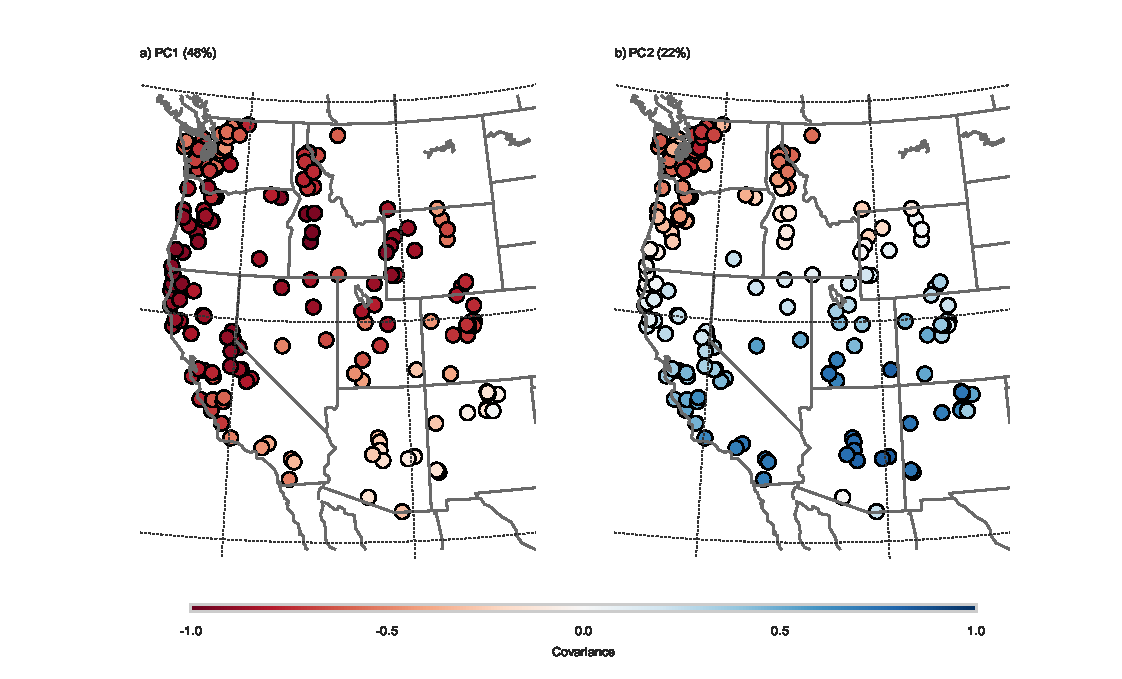
\includegraphics[width=190mm]{p1figures/fig1.pdf}}
\caption{Spatial pattern of leading PCs mapped as covariance of streamflow PC1 and PC2 on standardized streamflow series (WY1975 - 2011). The percent value in figure title is the percent of streamflow variability accounted for by the PC.}
\label{fig:eofs}
\end{figure}

Global SSTs and Northern Hemisphere 500 mb geopotential height fields were used to identify climate variability associated with western US streamflow. We used 500 mb geopotential height data obtained from the Twentieth Century Reanalysis Version 2 (20CR) \citep{1compo_twentieth_2011}. The 500 mb level is used because it is above the mountainous, higher elevations of the western US. SSTs used are from the NOAA Extended Reconstructed Sea Surface Temperature V3b (ERSST) \citep{1smith_improvements_2008}. Both products have a  2\textdegree by 2\textdegree spatial resolution. The cool-season is the primary period for moisture delivery into western US river basins. Our analysis focuses on this seasonal moisture delivery as a primary influence on interannual streamflow variability. However, we examine all seasons to identify possible persistent or lagged relationships in geopotential height and SST fields influence. Annual season-averaged 500 mb geopotential height anomalies are used for summer prior to the onset of the water year (JJA), and for the fall (SON), winter (DJF), and spring (MAM) of the water year itself. These season averages were created from 20CR monthly average ensemble means. SST fields use the same seasons, averaged from monthly values but these values are linear-detrended anomalies. Note that there is considerably more uncertainty in the 20CR ensemble data prior to 1950 \citep{1compo_twentieth_2011}. To check against bias in 20CR and ERSST, we repeated analyses from 1983 - 2011 using HCDN streamflow data with geopotential height fields from ERA-Interim reanalysis \citep{1dee_era-interim_2011, 1european_centre_for_medium-range_weather_forecasts_era-interim_2012} and SST fields from Optimum Interpolation Sea Surface Temperature analysis V2 \citep{1reynolds_daily_2007}. The results were comparable to that produced with 20CR and ERSST.

\section{Methods}

Each annual streamflow series was transformed into standardized values from the common period of analysis. This standardization addresses potentially differing streamflow distribution scales, shapes, and spreads. We were concerned that these differences might otherwise bias extreme values in a PCA conducted on streamflow series from different western US basins. Values were standardized by fitting each streamflow series to a gamma distribution and then inverting the corresponding probabilities to a Gaussian distribution. In short, this transformation is similar to the Standardized Precipitation Index \citep{1mckee_relationship_1993} for precipitation, though applied to streamflow data. We used a Kolmogorov-Smirnov goodness-of-fit test for each gage against a fitted gamma distribution. Only one gage in California did not reject the null hypothesis that the distribution is identical to a fitted gamma distribution ($\alpha = 0.05$). In addition, we repeated this study's analysis using a $Z$-score standardization of streamflow. Despite our concern, $Z$-score standardization produced similar results.

PCA was based on singular value decomposition of the standardized streamflow covariance matrix. This PCA allowed us to define the dominant patterns of variability in western US streamflow, with each component being independent (i.e. orthogonal) from other components. Significant, leading PCs were identified by evaluating the explained variance and separation from other components \citep{1north_sampling_1982}. The PCs are standardized to unit variance. The leading empirical orthogonal functions, the spatial expression of the leading PC patterns, were mapped by plotting the covariance of a PC with the standardized streamflow data. See Wilks \citet{1wilks_statistical_2006} for a review of these methods.

The leading patterns of streamflow variability were used to identify relationships with  seasonal SST and 500 mb geopotential height fields using two methods. First, point-correlation maps were generated to identify simple linear relationships between the leading streamflow PC time series and the SST and geopotential height fields. Pearson product-moment correlation coefficients for each leading PC and field grid point were mapped and local, statistical significance tested ($\alpha = 0.05$). 

Point-correlation maps were supplemented with non-parametric composite analysis maps. These maps identify areas in a SST or geopotential height field that exhibit statistically significant mean differences between positive and negative signs of a streamflow PC time series. These maps were created for each leading streamflow PC for each climate field. Differences between the patterns for years with negative and positive PC loadings were tested using Welch's unequal variance $t$-test for each grid point in the field. This procedure tests against the null hypothesis that the two composite samples have equal means, while accounting for the variance of each sample. Grid points that exhibited consistent changes with streamflow PCs, rejecting the null hypothesis ($\alpha = 0.05$), were mapped.

Our analysis was performed in Python using several Open Source scientific software libraries \citep{1hunter_matplotlib:_2007, 1van_der_walt_numpy_2011, 1dawson_eofs:_2016}. Code used in our data collection and analysis is available online (\url{https://github.com/brews/riverpca}) or by request from the corresponding author.

\section{Results and discussion}

Interannual western US streamflow is characterized by two leading and well-separated patterns of variability in the past century (Figure~\ref{fig:eofs}). The leading pattern, or principal component (PC1), accounts for approximately one half of streamflow variability (48\%) while the second pattern (PC2) accounts for approximately one quarter of variability (22\%). A linear combination of these two patterns accounts for roughly three quarters of the variability in standardized streamflow. Time series of PC1 and PC2 are shown in supporting information Figure~\ref{sfig:pctimeseries}.% The two leading PCs for streamflow are including in supporting information Data Set 1.

The leading patterns of streamflow variability have distinct spatial characteristics that relate to cool-season moisture delivery. PC1 is associated with widespread flow anomalies of the same sign across western US streamflow (Figure~\ref{fig:eofs}a). This widespread single-sign covariability has been noted previously in western US streamflow, snowpack, and coastal precipitation analyses \citep{1mcguirk_century_1982, 1cayan_influence_1989, 1lins_regional_1997, 1mccabe_primary_2002}. The spatial expression of PC2 (Figure~\ref{fig:eofs}b) is a contrasting north-south seesaw or dipole pattern, a well-established characteristic of the western US linear climate response to ENSO in the cool-season \citep{1dettinger_northsouth_1998, 1wise_spatiotemporal_2010}. These two streamflow patterns and their climate relationships are replicated in the WY1925 - 2011 PCA. Analysis for this longer PCA are available in supporting information.

\subsection{Mid-latitude atmospheric circulation and blocking pressure anomalies in PC1}

The correlations between the leading pattern of streamflow variability (PC1) and 500 mb geopotential height from fall through spring (Figure~\ref{fig:corrhgt}b-d) reflects the pattern's association with cool-season synoptic-scale atmospheric circulation. No significant, organized relationship is evident in the summer correlation map (Figure~\ref{fig:corrhgt}a). During fall and winter, the significant positive correlations over the North American Cordillera and northwest coast are flanked by negative correlations near the Aleutian Islands and eastern North America, reflecting mid-latitude atmospheric circulation wave-train dynamics (Figure~\ref{fig:corrhgt}b-c). The area of significant positive correlation near the northwest US, specifically, is found in fall (Figure~\ref{fig:corrhgt}b), winter (Figure~\ref{fig:corrhgt}c), and spring (Figure~\ref{fig:corrhgt}d). This suggests that widespread low streamflow is associated with anomalously high pressure, characteristic of a persistent ridge. This is a pressure anomaly which can preferentially block, separate, or suppress incoming cool-season moisture from the Pacific. The high PC1 value in 1977, a year with an intense ridge and widespread streamflow drought, is an example of this (see supporting information Figure \ref{sfig:pctimeseries}a). Inversely, negative pressure anomalies over this area are associated with widespread high streamflow anomalies. This relationship with geopotential height is inverted further to the south near the Baja California peninsula in winter and spring (Figure~\ref{fig:corrhgt}c-d). The consistency and strength of the anomalies near the northwest US is further emphasized in the PC1 composite test for 500 mb geopotential heights from fall through spring (Figure~\ref{fig:comphgt}b-d), demonstrating statistically significant geopotential height differences between positive and negative PC1 years (i.e. years of widespread high and low streamflow anomalies). These composite maps show significance near the North American Pacific coast, but not near the semi-permanent Aleutian low.

\begin{figure}[ht]
\centering
\centerline{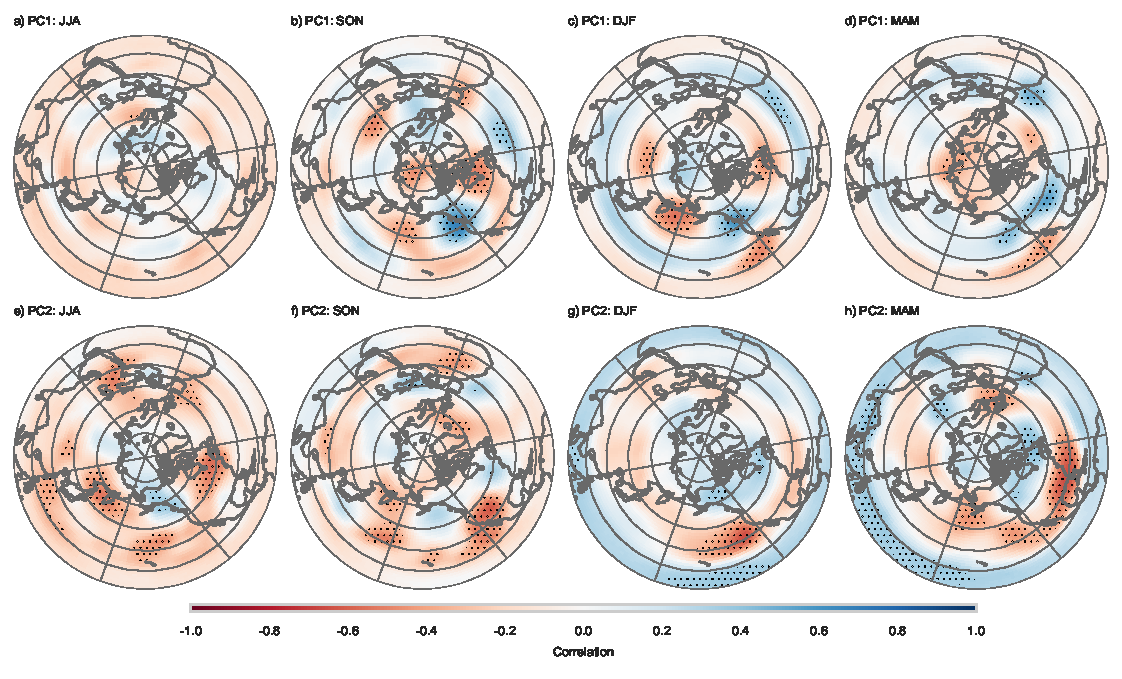
\includegraphics[width=190mm]{p1figures/fig2.pdf}}
\caption{Point correlation map of streamflow PC1 and PC2 on 500 mb geopotential height anomaly fields for each season in the Northern Hemisphere (WY1975 - 2011). Stippled areas show local statistical significance ($\alpha = 0.05$).}
\label{fig:corrhgt}
\end{figure}

\begin{figure}[ht]
\centering
\centerline{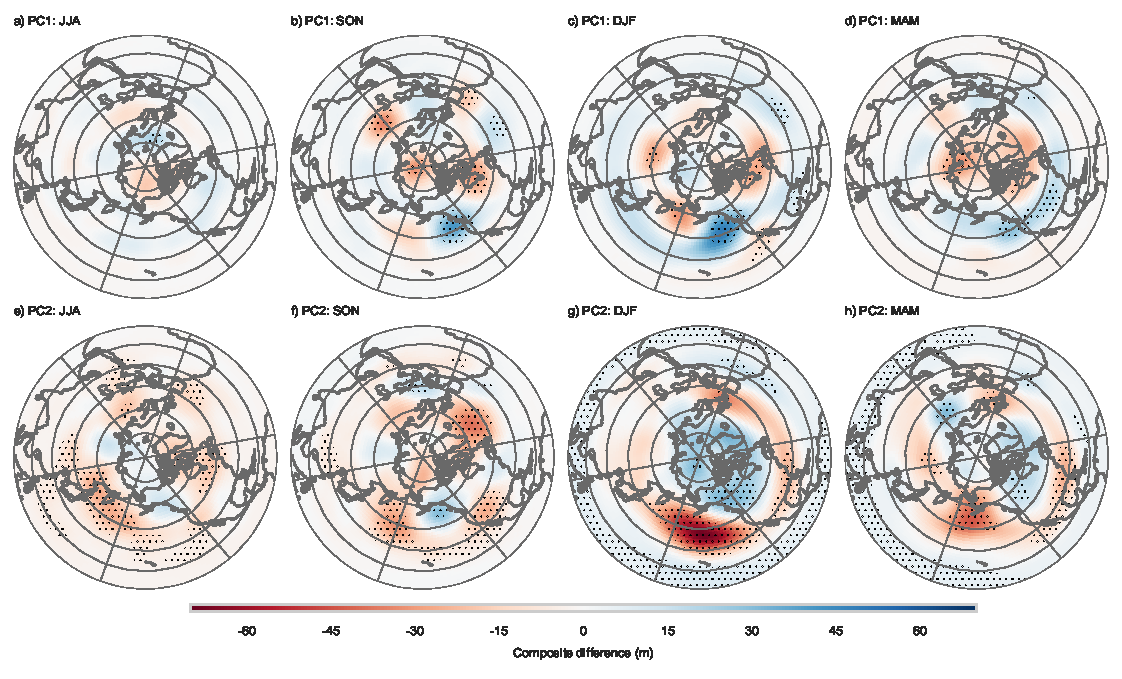
\includegraphics[width=190mm]{p1figures/fig3.pdf}}
\caption{Composite mean difference 500 mb geopotential height anomaly for each season. This difference is the composite of positive streamflow PC years minus negative PC years for PC1 and PC2. Stippled areas show composite means with local statistical significance ($\alpha = 0.05$).}
\label{fig:comphgt}
\end{figure}

The widespread covariability in streamflow has been associated with the semi-permanent Aleutian low \citep{1cayan_influence_1989, 1lins_regional_1997} and this is shown in our results: a center of negative correlation near the Aleutian islands in fall and winter (Figure~\ref{fig:corrhgt}b-c), but not spring (Figure~\ref{fig:corrhgt}d). Interestingly, geopotential height anomalies at the Aleutian Islands do not show widespread significant difference between positive and negative PC1 years in any season (Figure~\ref{fig:comphgt}a-d). This suggests that a relationship does exist with pressure anomalies near the Aleutian Islands, however, widespread variability in western US streamflow may have a more immediate and consistent relationship with the anomalies relating to North American Pacific coast ridging behavior.

The leading pattern of streamflow variability does not have widespread significant correlations with SSTs (Figure~\ref{fig:corrsst}a-d), especially when compared to PC2 (Figure~\ref{fig:corrhgt}e-h). Positive North Pacific SST correlations with PC1 are found in the winter (Figure~\ref{fig:corrsst}c) along the coast of southern Alaska and British Columbia with opposite-sign SST correlations from the central North Pacific to northeast Asia. More generally, negative SST correlations in the central north Pacific are found in fall, winter, and spring (Figure~\ref{fig:corrsst}b-d). This pattern hints at a possible relation between west-wide streamflow and the leading mode of variability for North Pacific SST \citep{1mantua_pacific_2002}. This relationship has been proposed for western US snowpack variability \citep{1mccabe_primary_2002} and in earlier streamflow studies \citep [e.g., ][]{1tootle_coupled_2005, 1tootle_relationships_2006, 1sagarika_pacific_2016}. However, the fall-through-spring SST composite-test map for PC1 shows no corresponding widespread areas of the North Pacific with statistically significant differences between the years of positive and negative PC1 values (Figure~\ref{fig:compsst}b-d), though PC1 in the WY1925 PCA does have an area of significance in winter (supporting information Figure ~\ref{sfig:compsst}). PC1 may be influenced by North Pacific SSTs, but our results suggest that organized SSTs in the North Pacific are not a consistent driver of interannual covariability in streamflow across the western US.

\begin{figure}[ht]
\centering
\centerline{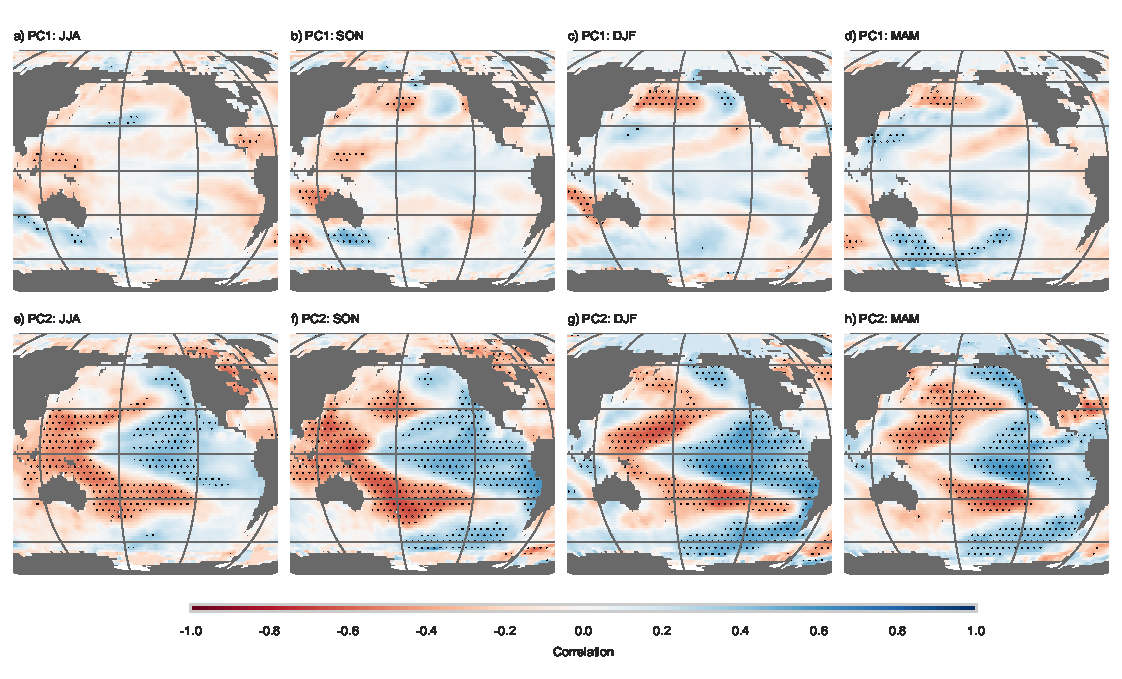
\includegraphics[width=190mm]{p1figures/fig4.pdf}}
\caption{Point correlation map of streamflow PC1 and PC2 on detrended SST anomaly fields for each season (WY1975 - 2011). Stippled areas show local statistical significance ($\alpha = 0.05$).}
\label{fig:corrsst}
\end{figure}

\begin{figure}[ht]
\centering
\centerline{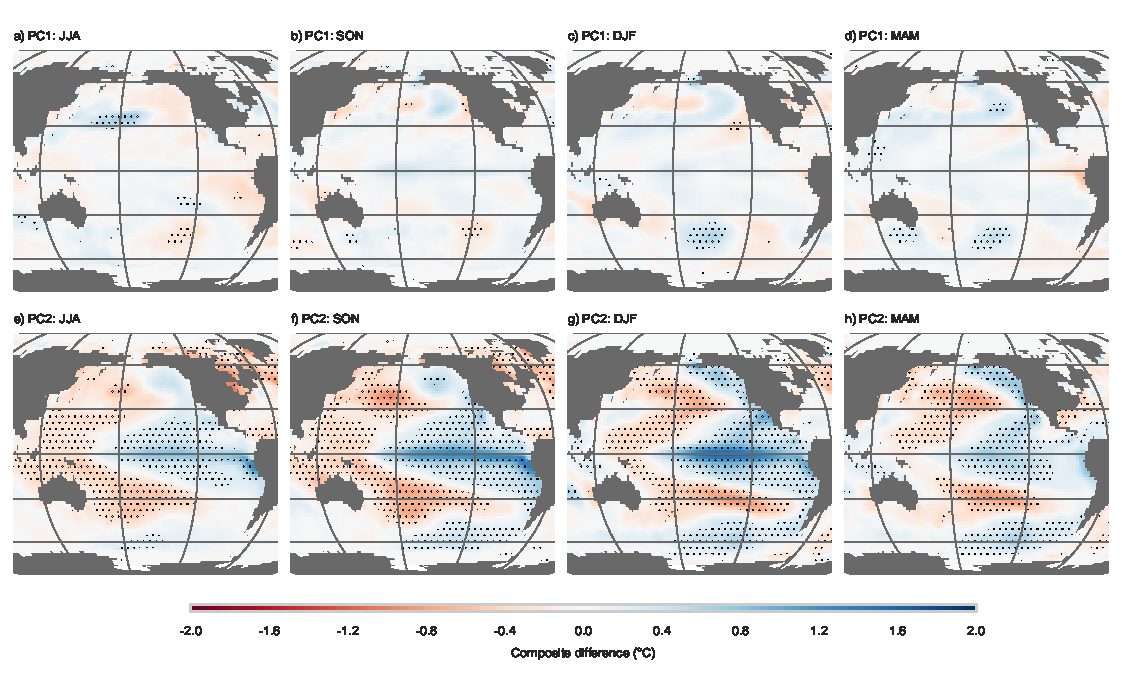
\includegraphics[width=190mm]{p1figures/fig5.pdf}}
\caption{Composite mean difference detrended SST anomaly for each season. This difference is the composite of positive streamflow PC years minus negative PC years for PC1 and PC2. Stippled areas show composite means with local statistical significance ($\alpha = 0.05$).}
\label{fig:compsst}
\end{figure}

\subsection{ENSO teleconnection in PC2}

Point-correlation maps of the second leading pattern of streamflow variability with winter 500 mb geopotential height anomalies show an ENSO-like influence with significant correlations to higher latitudes near Alaska and northwest Canada, and a wide area of opposite sign correlation off the California coast (Figure~\ref{fig:corrhgt}g). Correlation maps with winter SST anomalies show significant correlations across the equatorial Pacific that extend symmetrically into the higher latitudes (Figure~\ref{fig:corrsst}g). This ENSO-like pattern is also found in the PC2 composite maps for SST anomalies in all seasons (Figure~\ref{fig:compsst}e-h).

Geopotential height correlation maps show areas of significant correlation establishing and sustaining a linear relationship with PC2, leading and lagging winter by several months (Figure~\ref{fig:corrhgt}e-h). A similar lag-lead relationship is found with SST anomalies (Figure~\ref{fig:corrsst}e-h). The SST correlations cover considerably more area through each of the seasons (Figure~\ref{fig:corrsst}e-h). This relationship begins as early as summer (JJA) and continues through spring (MAM). Explaining approximately one-quarter of the streamflow variability, ENSO state is clearly important for seasonal forecasts of streamflow, yet potentially limited as a predictor when used by itself.

\subsection{Implications for widespread streamflow anomalies}

Our results show that roughly 50\% of interannual streamflow variability in the western US can be expressed as widespread streamflow anomalies without consistent need for Pacific SST forcing. Orthogonal to this pattern, approximately 25\% of interannual streamflow variability is linked to the well-established western US hydroclimate response to ENSO teleconnections. Rather than stressing the role of the ENSO or North Pacific multidecadal variability \citep [e.g., ][]{1tootle_coupled_2005, 1sagarika_pacific_2016}, our results stress the potential influence of internal climate variability and the role of persistent coastal-ridge pressure anomalies in the eastern North Pacific as a consistent and direct source of cohesion for multi-basin streamflow variability. These mechanisms closely correspond to those discussed in recent drought studies \citep [e.g., ][]{1cook_worst_2014, 1seager_atmosphere_2014, 1teng_causes_2016, 1wise_five_2016}. We show that these two streamflow patterns have likely been a robust characteristic of streamflow variability through to the early half of the twentieth century.

These results suggest that widespread interannual streamflow anomalies may be especially difficult to anticipate with seasonal hydroclimate forecasts because the widespread streamflow variability in PC1 is not consistently related to ENSO variability, nor does it show strong and widespread seasonal lag-lead correlations with Pacific SSTs to the extent that we have seen with PC2's reflection of ENSO-like teleconnections. In contrast, ENSO-related anomalies in PC2 may be more readily forecasted, but this variability is associated with approximately one-quarter of the variability in Western US streamflow.

Years with extremely widespread and intense streamflow drought relating to persistent coastal ridges, such as 1977, can be interpreted as an extreme expression of PC1, which we associate with semi-permanent 500 mb ridging along the Pacific coast and a deepening of Aleutian low anomalies. Future climate change is projected to significantly shift semi-permanent air masses and mid-latitude storm tracks \citep[e.g., ][]{1yin_consistent_2005, 1lu_expansion_2007, 1scheff_twenty-first-century_2012, 1langenbrunner_patterns_2015, 1choi_uncertainty_2016}. If these shifts in North Pacific atmospheric circulation are realized, it could change the way that semi-permanent air masses impact widespread streamflow anomalies. Unfortunately, we suspect that it will be a challenge to project what these changes will be and how these changes will affect water management because there are a number of outstanding uncertainties \citep[e.g., ][]{1reclamation_bureau_of_reclamation_west-wide_2016}, such as that in multimodel climate projections in the eastern North Pacific \citep[e.g., ][]{1langenbrunner_patterns_2015, 1choi_uncertainty_2016}.

\section{Conclusion}

Our analysis suggests that widespread western US streamflow anomalies are most strongly associated with mid-latitude atmospheric circulation relating to persistent atmospheric ridges, independent of direct interaction from ENSO and equatorial Pacific SSTs. This result appears to be a consistent characteristic of the instrumental streamflow record in the past century, accounting for roughly one-half of the variance in western US annual streamflow. Roughly one-quarter of streamflow variability is associated with ENSO-like teleconnections. Because ENSO-state provides forecasting skill, this influence on streamflow may be anticipated seasons in advance. However, ENSO-driven streamflow anomalies can be complicated by significant and more spatially widespread influence from mid-latitude atmospheric circulation, as seen in the extreme 1977 drought. This western US-wide influence from mid-latitude circulation is not as strongly associated with Pacific SSTs and will likely be a challenge to anticipate in seasonal hydroclimate forecasts. These patterns in streamflow may changes with shifting North Pacific atmospheric circulation under future climate change.

\section{Acknowledgements}

Thanks to Joellen Russell, Elizabeth Ritchie, Chris Castro, Kevin Anchukaitis, Andrew Comrie, and Dave Meko. Thanks also to our anonymous reviewers for their feedback. NOAA ERSST and 20th Century Reanalysis data were provided by the NOAA/OAR/ESRL PSD, Boulder, Colorado, USA (http://www.esrl.noaa.gov/psd/). This research was supported by the US Bureau of Reclamation WaterSmart program (Agreement \# R11 AP 81 457). 

% \bibliographystyle{ametsoc2014}
% \bibliography{references}

\begin{thebibliography}{59}
\providecommand{\natexlab}[1]{#1}
\expandafter\ifx\csname urlstyle\endcsname\relax
  \providecommand{\doi}[1]{doi:\discretionary{}{}{}#1}\else
  \providecommand{\doi}{doi:\discretionary{}{}{}\begingroup
  \urlstyle{rm}\Url}\fi

\bibitem[{\textit{Cayan and Peterson}(1989)}]{1cayan_influence_1989}
Cayan, D.~R., and D.~H. Peterson (1989), The {Influence} of {North} {Pacific}
  {Atmospheric} {Circulation} on {Streamflow} in the {West}, in \textit{Aspects
  of {Climate} {Variability} in the {Pacific} and the {Western} {Aimericas}},
  edited by D.~H. Peterson, pp. 375--397, American Geophysical Union,
  Washington, D. C., doi: 10.1029/GM055p0375.

\bibitem[{\textit{Cayan et~al.}(1999)\textit{Cayan, Redmond, and
  Riddle}}]{1cayan_enso_1999}
Cayan, D.~R., K.~T. Redmond, and L.~G. Riddle (1999), {ENSO} and {Hydrologic}
  {Extremes} in the {Western} {United} {States}, \textit{J. Clim.},
  \textit{12}(9), 2881--2893,
  \doi{10.1175/1520-0442(1999)012<2881:EAHEIT>2.0.CO;2}.

\bibitem[{\textit{Choi et~al.}(2016)\textit{Choi, Lu, Son, Frierson, and
  Yoon}}]{1choi_uncertainty_2016}
Choi, J., J.~Lu, S.-W. Son, D.~M.~W. Frierson, and J.-H. Yoon (2016),
  Uncertainty in future projections of the {North} {Pacific} subtropical high
  and its implication for {California} winter precipitation change, \textit{J.
  Geophys. Res. Atmos.}, \textit{121}(2), 2015JD023,858,
  \doi{10.1002/2015JD023858}.

\bibitem[{\textit{Compo et~al.}(2011)\textit{Compo, Whitaker, Sardeshmukh,
  Matsui, Allan, Yin, Gleason, Vose, Rutledge, Bessemoulin, Brannimann,
  Brunet, Crouthamel, Grant, Groisman, Jones, Kruk, Kruger, Marshall, Maugeri,
  Mok, Nordli, Ross, Trigo, Wang, Woodruff, and Worley}}]{1compo_twentieth_2011}
Compo et al. (2011), The {Twentieth} {Century} {Reanalysis} {Project},
  \textit{Q.J.R. Meteorol. Soc.}, \textit{137}(654), 1--28,
  \doi{10.1002/qj.776}.

\bibitem[{\textit{Cook et~al.}(2014)\textit{Cook, Seager, and
  Smerdon}}]{1cook_worst_2014}
Cook, B.~I., R.~Seager, and J.~E. Smerdon (2014), The worst {North} {American}
  drought year of the last millennium: 1934, \textit{Geophys. Res. Lett.},
  \textit{41}(20), 7298--7305, \doi{10.1002/2014GL061661}.

\bibitem[{\textit{Dawson}(2016)}]{1dawson_eofs:_2016}
Dawson, A. (2016), eofs: {A} {Library} for {EOF} {Analysis} of
  {Meteorological}, {Oceanographic}, and {Climate} {Data}, \textit{Journal of
  Open Research Software}, \textit{4}(1), \doi{10.5334/jors.122}.

\bibitem[{\textit{Dee et~al.}(2011)\textit{Dee, Uppala, Simmons, Berrisford,
  Poli, Kobayashi, Andrae, Balmaseda, Balsamo, Bauer, Bechtold, Beljaars,
  van~de Berg, Bidlot, Bormann, Delsol, Dragani, Fuentes, Geer, Haimberger,
  Healy, Hersbach, Hólm, Isaksen, Kållberg, Köhler, Matricardi, McNally,
  Monge-Sanz, Morcrette, Park, Peubey, de~Rosnay, Tavolato, Thépaut, and
  Vitart}}]{1dee_era-interim_2011}
Dee et al. (2011), The {ERA}-{Interim}
  reanalysis: configuration and performance of the data assimilation system,
  \textit{Q.J.R. Meteorol. Soc.}, \textit{137}(656), 553--597,
  \doi{10.1002/qj.828}.
  
\bibitem[{\textit{Dettinger et~al.}(2015)\textit{Dettinger, Udall, and
  Georgakakos}}]{1dettinger_western_2015}
Dettinger, M., B.~Udall, and A.~Georgakakos (2015), Western water and climate
  change, \textit{Ecological Applications}, \textit{25}(8), 2069--2093,
  \doi{10.1890/15-0938.1}.
  
\bibitem[{\textit{Dettinger et~al.}(1998)\textit{Dettinger, Cayan, Diaz, and
  Meko}}]{1dettinger_northsouth_1998}
Dettinger, M.~D., D.~R. Cayan, H.~F. Diaz, and D.~M. Meko (1998),
  North-{South} {Precipitation} {Patterns} in {Western} {North} {America} on
  {Interannual}-to-{Decadal} {Timescales}, \textit{J. Clim.}, \textit{11}(12),
  3095--3111, \doi{10.1175/1520-0442(1998)011<3095:NSPPIW>2.0.CO;2}.

\bibitem[{\textit{Diaz and Wahl}(2015)}]{1diaz_recent_2015}
Diaz, H.~F., and E.~R. Wahl (2015), Recent {California} {Water} {Year}
  {Precipitation} {Deficits}: {A} 440-{Year} {Perspective}, \textit{J.
  Climate}, \textit{28}(12), 4637--4652, \doi{10.1175/JCLI-D-14-00774.1}.

\bibitem[{\textit{{European Centre for Medium-Range Weather
  Forecasts}}(2012)}]{1european_centre_for_medium-range_weather_forecasts_era-interim_2012}
{European Centre for Medium-Range Weather Forecasts} (2012), {ERA}-{Interim}
  {Project}, {Monthly} {Means}.

\bibitem[{\textit{Hartmann}(2015)}]{1hartmann_pacific_2015}
Hartmann, D.~L. (2015), Pacific sea surface temperature and the winter of 2014,
  \textit{Geophys. Res. Lett.}, \textit{42}(6), 1894--1902,
  \doi{10.1002/2015GL063083}.

\bibitem[{\textit{Herring et~al.}(2014)\textit{Herring, Hoerling, Peterson, and
  Stott}}]{1herring_explaining_2014}
Herring, S.~C., M.~P. Hoerling, T.~C. Peterson, and P.~A. Stott (2014),
  Explaining {Extreme} {Events} of 2013 from a {Climate} {Perspective},
  \textit{Bull. Amer. Meteor. Soc.}, \textit{95}, S1--S104.

\bibitem[{\textit{Hoerling et~al.}(2009)\textit{Hoerling, Quan, and
  Eischeid}}]{1hoerling_distinct_2009}
Hoerling, M., X.-W. Quan, and J.~Eischeid (2009), Distinct causes for two
  principal {U}.{S}. droughts of the 20th century, \textit{Geophys. Res.
  Lett.}, \textit{36}(19), L19,708, \doi{10.1029/2009GL039860}.

\bibitem[{\textit{Hunter}(2007)}]{1hunter_matplotlib:_2007}
Hunter, J.~D. (2007), Matplotlib: {A} 2d {Graphics} {Environment},
  \textit{Computing in Science \& Engineering}, \textit{9}(3), 90--95,
  \doi{10.1109/MCSE.2007.55}.

\bibitem[{\textit{Langenbrunner et~al.}(2015)\textit{Langenbrunner, Neelin,
  Lintner, and Anderson}}]{1langenbrunner_patterns_2015}
Langenbrunner, B., J.~D. Neelin, B.~R. Lintner, and B.~T. Anderson (2015),
  Patterns of {Precipitation} {Change} and {Climatological} {Uncertainty} among
  {CMIP}5 {Models}, with a {Focus} on the {Midlatitude} {Pacific} {Storm}
  {Track}, \textit{J. Climate}, \textit{28}(19), 7857--7872,
  \doi{10.1175/JCLI-D-14-00800.1}.


\bibitem[{\textit{Lins}(1997)}]{1lins_regional_1997}
Lins, H.~F. (1997), Regional streamflow regimes and hydroclimatology of the
  {United} {States}, \textit{Water Resour. Res.}, \textit{33}(7), 1655--1667,
  \doi{10.1029/97WR00615}.

\bibitem[{\textit{Lins}(2012)}]{1lins_usgs_2012}
Lins, H.~F. (2012), {USGS} {Hydro}-{Climatic} {Data} {Network} 2009
  ({HCDN}-2009), \textit{Fact {Sheet} 3047}, U.S. Geological Survey.

\bibitem[{\textit{Liu and Alexander}(2007)}]{1liu_atmospheric_2007}
Liu, Z., and M.~Alexander (2007), Atmospheric bridge, oceanic tunnel, and
  global climatic teleconnections, \textit{Rev. Geophys.}, \textit{45}(2),
  \doi{10.1029/2005RG000172}.

\bibitem[{\textit{Lu et~al.}(2007)\textit{Lu, Vecchi, and
  Reichler}}]{1lu_expansion_2007}
Lu, J., G.~A. Vecchi, and T.~Reichler (2007), Expansion of the {Hadley} cell
  under global warming, \textit{Geophys. Res. Lett.}, \textit{34}(6), L06,805,
  \doi{10.1029/2006GL028443}.

\bibitem[{\textit{Mantua and Hare}(2002)}]{1mantua_pacific_2002}
Mantua, N., and S.~Hare (2002), The {Pacific} {Decadal} {Oscillation},
  \textit{J. Oceanogr.}, \textit{58}(1), 35--44, \doi{10.1023/A:1015820616384}.

\bibitem[{\textit{McCabe and Dettinger}(2002)}]{1mccabe_primary_2002}
McCabe, G.~J., and M.~D. Dettinger (2002), Primary {Modes} and {Predictability}
  of {Year}-to-{Year} {Snowpack} {Variations} in the {Western} {United}
  {States} from {Teleconnections} with {Pacific} {Ocean} {Climate}, \textit{J.
  Hydrometeor}, \textit{3}(1), 13--25,
  \doi{10.1175/1525-7541(2002)003<0013:PMAPOY>2.0.CO;2}.

\bibitem[{\textit{McGuirk}(1982)}]{1mcguirk_century_1982}
McGuirk, J.~P. (1982), A century of precipitation variability along the pacific
  coast of {North} {America} and its impact, \textit{Climatic Change},
  \textit{4}(1), 41, \doi{10.1007/BF02423312}.


\bibitem[{\textit{McKee et~al.}(1993)\textit{McKee, Doesken, and
  Kleist}}]{1mckee_relationship_1993}
McKee, T.~B., N.~J. Doesken, and J.~Kleist (1993), The relationship of drought
  frequency and druration to time scales, in \textit{Proceedings of the 8th
  {Conference} on {Applied} {Climatology}}, \textit{22}, vol.~17, pp. 179--183,
  American Meteorolical Society, Boston, MA.

\bibitem[{\textit{Meko et~al.}(2012)\textit{Meko, Woodhouse, and
  Morino}}]{1meko_dendrochronology_2012}
Meko, D.~M., C.~A. Woodhouse, and K.~Morino (2012), Dendrochronology and links
  to streamflow, \textit{Journal of Hydrology}, \textit{412-413}, 200--209,
  \doi{10.1016/j.jhydrol.2010.11.041}.

\bibitem[{\textit{North et~al.}(1982)\textit{North, Bell, Cahalan, and
  Moeng}}]{1north_sampling_1982}
North, G.~R., T.~L. Bell, R.~F. Cahalan, and F.~J. Moeng (1982), Sampling
  {Errors} in the {Estimation} of {Empirical} {Orthogonal} {Functions},
  \textit{Mon. Wea. Rev.}, \textit{110}(7), 699--706,
  \doi{10.1175/1520-0493(1982)110<0699:SEITEO>2.0.CO;2}.

\bibitem[{\textit{Reclamation}(2016a)}]{1reclamation_bureau_of_reclamation_secure_2016}
{Reclamation (Bureau of Reclamation)} (2016a), {SECURE} {Water} {Act} {Section}
  9503(c) - {Reclamation} {Climate} {Change} and {Water}. {Prepared} for
  {United} {States} {Congress}., \textit{Tech. rep.}, Bureau of Reclamation,
  Policy and Administration, Denver, CO.

\bibitem[{\textit{Reclamation}(2016b)}]{1reclamation_bureau_of_reclamation_west-wide_2016}
{Reclamation (Bureau of Reclamation)} (2016b), West-{Wide} {Climate} {Risk} {Assessments}:
  {Hydroclimate} {Projections}, \textit{Technical {Memorandum}
  86-68210-2016-01}, U.S. Bureau of Reclamation, Denver, CO.


\bibitem[{\textit{Redmond and Koch}(1991)}]{1redmond_surface_1991}
Redmond, K.~T., and R.~W. Koch (1991), Surface {Climate} and {Streamflow}
  {Variability} in the {Western} {United} {States} and {Their} {Relationship}
  to {Large}-{Scale} {Circulation} {Indices}, \textit{Water Resour. Res.},
  \textit{27}(9), 2381--2399, \doi{10.1029/91WR00690}.

\bibitem[{\textit{Reynolds et~al.}(2007)\textit{Reynolds, Smith, Liu, Chelton,
  Casey, and Schlax}}]{1reynolds_daily_2007}
Reynolds, R.~W., T.~M. Smith, C.~Liu, D.~B. Chelton, K.~S. Casey, and M.~G.
  Schlax (2007), Daily {High}-{Resolution}-{Blended} {Analyses} for {Sea}
  {Surface} {Temperature}, \textit{J. Clim.}, \textit{20}(22), 5473--5496,
  \doi{10.1175/2007JCLI1824.1}.

\bibitem[{\textit{Sagarika et~al.}(2016)\textit{Sagarika, Kalra, and
  Ahmad}}]{1sagarika_pacific_2016}
Sagarika, S., A.~Kalra, and S.~Ahmad (2016), Pacific {Ocean} {SST} and {Z}500
  climate variability and western {U}.{S}. seasonal streamflow, \textit{Int. J.
  Climatol.}, \textit{36}(3), 1515--1533, \doi{10.1002/joc.4442}.

\bibitem[{\textit{Scheff and
  Frierson}(2012)}]{1scheff_twenty-first-century_2012}
Scheff, J., and D.~Frierson (2012), Twenty-{First}-{Century} {Multimodel}
  {Subtropical} {Precipitation} {Declines} {Are} {Mostly} {Midlatitude}
  {Shifts}, \textit{J. Climate}, \textit{25}(12), 4330--4347,
  \doi{10.1175/JCLI-D-11-00393.1}.


\bibitem[{\textit{Schubert et~al.}(2004)\textit{Schubert, Suarez, Pegion,
  Koster, and Bacmeister}}]{1schubert_cause_2004}
Schubert, S.~D., M.~J. Suarez, P.~J. Pegion, R.~D. Koster, and J.~T. Bacmeister
  (2004), On the {Cause} of the 1930s {Dust} {Bowl}, \textit{Science},
  \textit{303}(5665), 1855--1859, \doi{10.1126/science.1095048}.

\bibitem[{\textit{Seager and Hoerling}(2014)}]{1seager_atmosphere_2014}
Seager, R., and M.~Hoerling (2014), Atmosphere and {Ocean} {Origins} of {North}
  {American} {Droughts}, \textit{J. Clim.}, \textit{27}(12), 4581--4606,
  \doi{10.1175/JCLI-D-13-00329.1}.

\bibitem[{\textit{Seager et~al.}(2005)\textit{Seager, Kushnir, Herweijer, Naik,
  and Velez}}]{1seager_modeling_2005}
Seager, R., Y.~Kushnir, C.~Herweijer, N.~Naik, and J.~Velez (2005), Modeling of
  {Tropical} {Forcing} of {Persistent} {Droughts} and {Pluvials} over {Western}
  {North} {America}: 1856-2000, \textit{J. Clim.}, \textit{18}(19),
  4065--4088, \doi{10.1175/JCLI3522.1}.

\bibitem[{\textit{Seager et~al.}(2008)\textit{Seager, Kushnir, Ting, Cane,
  Naik, and Miller}}]{1seager_would_2008}
Seager, R., Y.~Kushnir, M.~Ting, M.~Cane, N.~Naik, and J.~Miller (2008), Would
  {Advance} {Knowledge} of 1930s {SSTs} {Have} {Allowed} {Prediction} of the
  {Dust} {Bowl} {Drought}?, \textit{J. Clim.}, \textit{21}(13), 3261--3281,
  \doi{10.1175/2007JCLI2134.1}.

\bibitem[{\textit{Seager et~al.}(2014)\textit{Seager, Hoerling, Schubert, Wang,
  Lyon, Kumar, Nakamura, and Henderson}}]{1seager_causes_2014}
Seager, R., M.~Hoerling, S.~Schubert, H.~Wang, B.~Lyon, A.~Kumar, J.~Nakamura,
  and N.~Henderson (2014), Causes and {Predictability} of the 2011 to 2014
  {California} {Drought}, \textit{Tech. rep.}, National Oceanic and Atmospheric
  Administration, Washington, D.C.

\bibitem[{\textit{Seager et~al.}(2015)\textit{Seager, Hoerling, Schubert, Wang,
  Lyon, Kumar, Nakamura, and Henderson}}]{1seager_causes_2015}
Seager, R., M.~Hoerling, S.~Schubert, H.~Wang, B.~Lyon, A.~Kumar, J.~Nakamura,
  and N.~Henderson (2015), Causes of the 2011-14 {California} {Drought},
  \textit{J. Climate}, \textit{28}(18), 6997--7024,
  \doi{10.1175/JCLI-D-14-00860.1}.

\bibitem[{\textit{Smith et~al.}(2008)\textit{Smith, Reynolds, Peterson, and
  Lawrimore}}]{1smith_improvements_2008}
Smith, T.~M., R.~W. Reynolds, T.~C. Peterson, and J.~Lawrimore (2008),
  Improvements to {NOAA}'s {Historical} {Merged} {Land}-{Ocean} {Surface}
  {Temperature} {Analysis} (1880-2006), \textit{J. Clim.}, \textit{21}(10),
  2283--2296, \doi{10.1175/2007JCLI2100.1}.

\bibitem[{\textit{Swain}(2015)}]{1swain_tale_2015}
Swain, D.~L. (2015), A tale of two {California} droughts: {Lessons} amidst
  record warmth and dryness in a region of complex physical and human
  geography, \textit{Geophys. Res. Lett.}, p. 2015GL066628,
  \doi{10.1002/2015GL066628}.

\bibitem[{\textit{Teng and Branstator}(2016)}]{1teng_causes_2016}
Teng, H., and G.~Branstator (2016), Causes of extreme ridges that induce
  {California} droughts, \textit{J. Climate}, \doi{10.1175/JCLI-D-16-0524.1}.

\bibitem[{\textit{Tootle and Piechota}(2006)}]{1tootle_relationships_2006}
Tootle, G.~A., and T.~C. Piechota (2006), Relationships between {Pacific} and
  {Atlantic} ocean sea surface temperatures and {U}.{S}. streamflow
  variability, \textit{Water Resour. Res.}, \textit{42}(7), W07,411,
  \doi{10.1029/2005WR004184}.

\bibitem[{\textit{Tootle et~al.}(2005)\textit{Tootle, Piechota, and
  Singh}}]{1tootle_coupled_2005}
Tootle, G.~A., T.~C. Piechota, and A.~Singh (2005), Coupled oceanic-atmospheric
  variability and {U}.{S}. streamflow, \textit{Water Resour. Res.},
  \textit{41}(12), W12,408, \doi{10.1029/2005WR004381}.

\bibitem[{\textit{van~der Walt et~al.}(2011)\textit{van~der Walt, Colbert, and
  Varoquaux}}]{1van_der_walt_numpy_2011}
van~der Walt, S., S.~C. Colbert, and G.~Varoquaux (2011), The {NumPy} {Array}:
  {A} {Structure} for {Efficient} {Numerical} {Computation}, \textit{Computing
  in Science \& Engineering}, \textit{13}(2), 22--30,
  \doi{10.1109/MCSE.2011.37}.

\bibitem[{\textit{Wang et~al.}(2014{\natexlab{a}})\textit{Wang, Schubert,
  Koster, Ham, and Suarez}}]{1wang_role_2014}
Wang, H., S.~Schubert, R.~Koster, Y.-G. Ham, and M.~Suarez
  (2014{\natexlab{a}}), On the {Role} of {SST} {Forcing} in the 2011 and 2012
  {Extreme} {U}.{S}. {Heat} and {Drought}: {A} {Study} in {Contrasts},
  \textit{J. Hydrometeor}, \textit{15}(3), 1255--1273,
  \doi{10.1175/JHM-D-13-069.1}.

\bibitem[{\textit{Wang et~al.}(2014{\natexlab{b}})\textit{Wang, Hipps, Gillies,
  and Yoon}}]{1wang_probable_2014}
Wang, S.-Y., L.~Hipps, R.~R. Gillies, and J.-H. Yoon (2014{\natexlab{b}}),
  Probable causes of the abnormal ridge accompanying the 2013-2014
  {California} drought: {ENSO} precursor and anthropogenic warming footprint,
  \textit{Geophys. Res. Lett.}, \textit{41}(9), 2014GL059,748,
  \doi{10.1002/2014GL059748}.

\bibitem[{\textit{Wilks}(2006)}]{1wilks_statistical_2006}
Wilks, D. (2006), \textit{Statistical {Methods} in the {Atmospheric}
  {Sciences}}, International geophysics series, 2nd ed., Academic Press,
  London, UK.

\bibitem[{\textit{Wise}(2010)}]{1wise_spatiotemporal_2010}
Wise, E.~K. (2010), Spatiotemporal variability of the precipitation dipole
  transition zone in the western {United} {States}, \textit{Geophys. Res.
  Lett.}, \textit{37}(7), L07,706, \doi{10.1029/2009GL042193}.

\bibitem[{\textit{Wise}(2016)}]{1wise_five_2016}
Wise, E.~K. (2016), Five centuries of {U}.{S}. {West} {Coast} drought:
  {Occurrence}, spatial distribution, and associated atmospheric circulation
  patterns, \textit{Geophys. Res. Lett.}, \textit{43}(9), 2016GL068,487,
  \doi{10.1002/2016GL068487}.

\bibitem[{\textit{Wise et~al.}(2014)\textit{Wise, Wrzesien, Dannenberg, and
  McGinnis}}]{1wise_cool-season_2014}
Wise, E.~K., M.~L. Wrzesien, M.~P. Dannenberg, and D.~L. McGinnis (2014),
  Cool-{Season} {Precipitation} {Patterns} {Associated} with {Teleconnection}
  {Interactions} in the {United} {States}, \textit{J. Appl. Meteor. Climatol.},
  \textit{54}(2), 494--505, \doi{10.1175/JAMC-D-14-0040.1}.
  
\bibitem[{\textit{Yin}(2005)}]{1yin_consistent_2005}
Yin, J.~H. (2005), A consistent poleward shift of the storm tracks in
  simulations of 21st century climate, \textit{Geophys. Res. Lett.},
  \textit{32}(18), L18,701, \doi{10.1029/2005GL023684}.

\end{thebibliography}

\chapter{Supplementary Information for Pacific SSTs, mid-latitude atmospheric circulation, and widespread interannual anomalies in Western US streamflow}

% \section*{Contents}
% %%%Remove or add items as needed%%%
% \begin{enumerate}
% \item Figures S1 to S8
% \end{enumerate}

% \section*{Additional Supporting Information (Files uploaded separately)}

% \begin{enumerate}
% \item Captions for Datasets S1 to S3
% \end{enumerate}

% \section*{Introduction}


% This supporting information includes data sets of principal components produced by the study, flow gage series, and additional figures. The data sets include the two leading principal component time series from WY1925 - 2011 and WY1975 - 2011. Additionally, we include files will all the USGS HCDN gage series used in the WY 1925 and WY1975 analysis. The additional figures describe the spatial distribution for the distribution of HCDN gages over different periods of time, and present results for the WY1925 PCA including correlation and composite maps from ensemble mean reanalysis data.

% \section*{Data Set S1.}

% Comma-delimited file of USGS HCDN gages used in the WY1975 - 2011 PCA. Column header gives the USGS site ID for each gage. Values are water-year average flow (ft$^3$ s$^{-1}$).


% \section*{Data Set S2.}

% Comma-delimited file of USGS HCDN gages used in the WY1925 - 2011 PCA. Column header gives the USGS site ID for each gage. Values are water-year average flow (ft$^3$ s$^{-1}$).


% \section*{Data Set S3.}

% Comma-delimited file of the two leading streamflow principal components from our WY1975 - 2011 and WY1925 - 2011 analysis.

\begin{figure}[ht]
\centering
\centerline{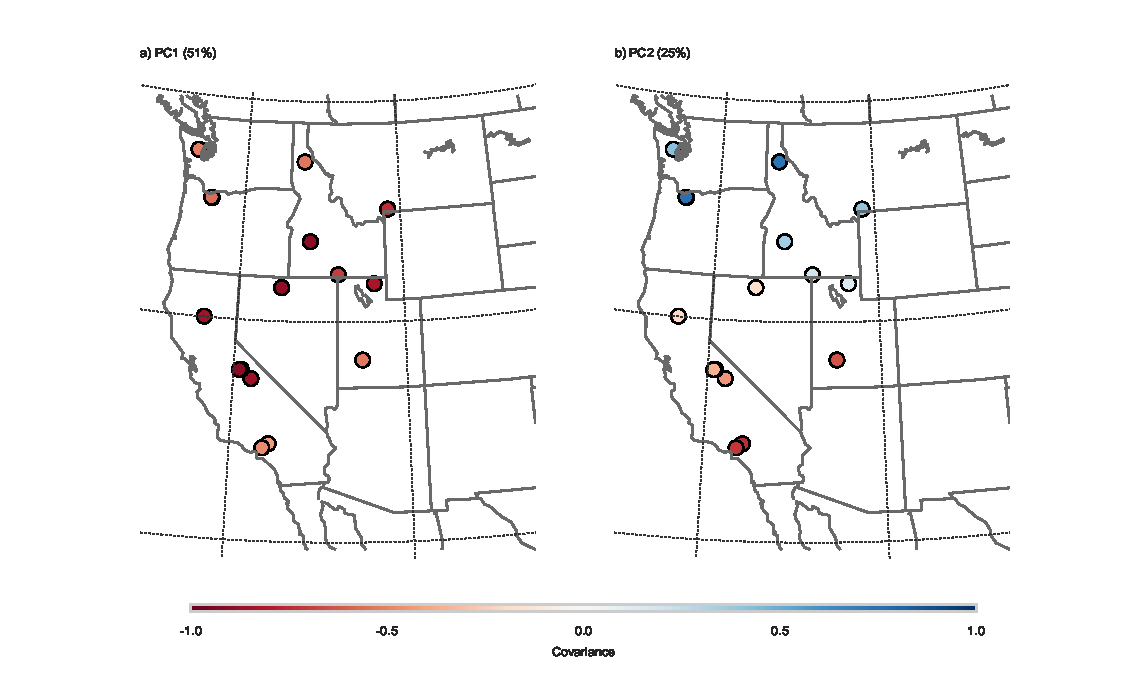
\includegraphics[width=190mm]{p1figures/s1.pdf}}
\caption{Spatial pattern of leading PC1 and PC2 as in Figure 1, but using streamflow data from WY1925 - 2011. These PCs are essentially replicated in the WY1975 - 2011 analysis.}
\label{sfig:eofs1925}
\end{figure}

\begin{figure}[ht]
\centering
\centerline{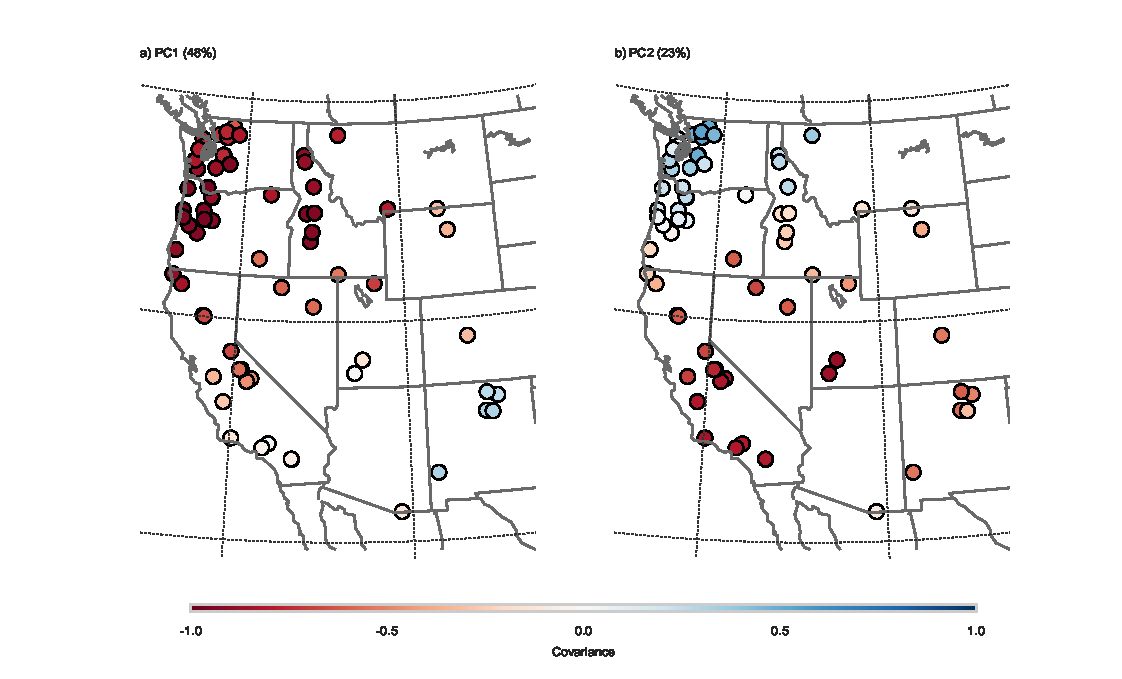
\includegraphics[width=190mm]{p1figures/s2.pdf}}
\caption{Spatial pattern of leading PC1 and PC2 as in Figure 1, but using streamflow data from WY1950 – 2011. Note the spatial pattern of PC1 differs slightly from PC1 in streamflow data beginning in WY1925 (Figure~\ref{sfig:eofs1925}) and WY1975 (Figure \ref{fig:eofs}), showing a stronger "dipole" ENSO-like influence. This was not replicated in our other periods of analysis.}
\label{sfig:eofs1950}
\end{figure}

\begin{figure}[ht]
\centering
\centerline{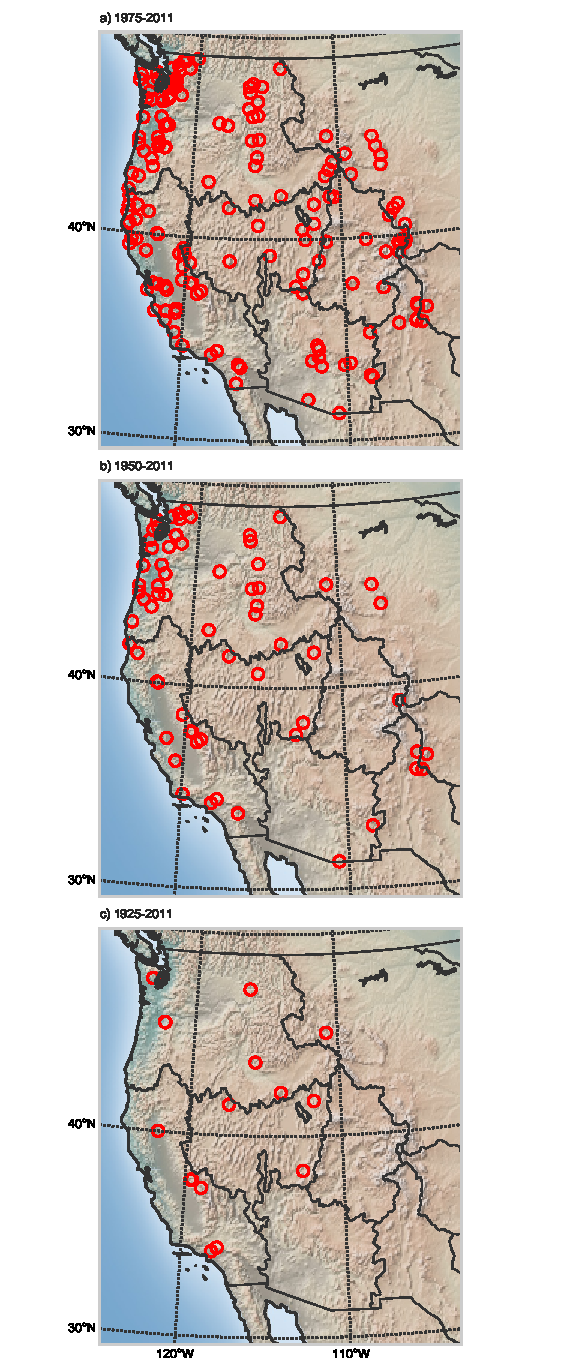
\includegraphics[width=70mm]{p1figures/s3.pdf}}
\caption{Spatial distribution of HCDN gages across western US basins with complete records for three time periods WY1975 - 2011, WY1950 - 2011, and WY1925 - 2011. WY1975 - 2011 (a) has gages across the western US but with clustering near the Pacific coast. With the mid-century (b) we loose gages in the inter-mountain region and have a relatively larger number of gages along the Pacific coast, and especially the Pacific Northwest. WY1925 - 2011 (c) has a relatively sparse, though spatially even, distribution.}
\label{sfig:gagedistribution}
\end{figure}

\begin{figure}[ht]
\centering
\centerline{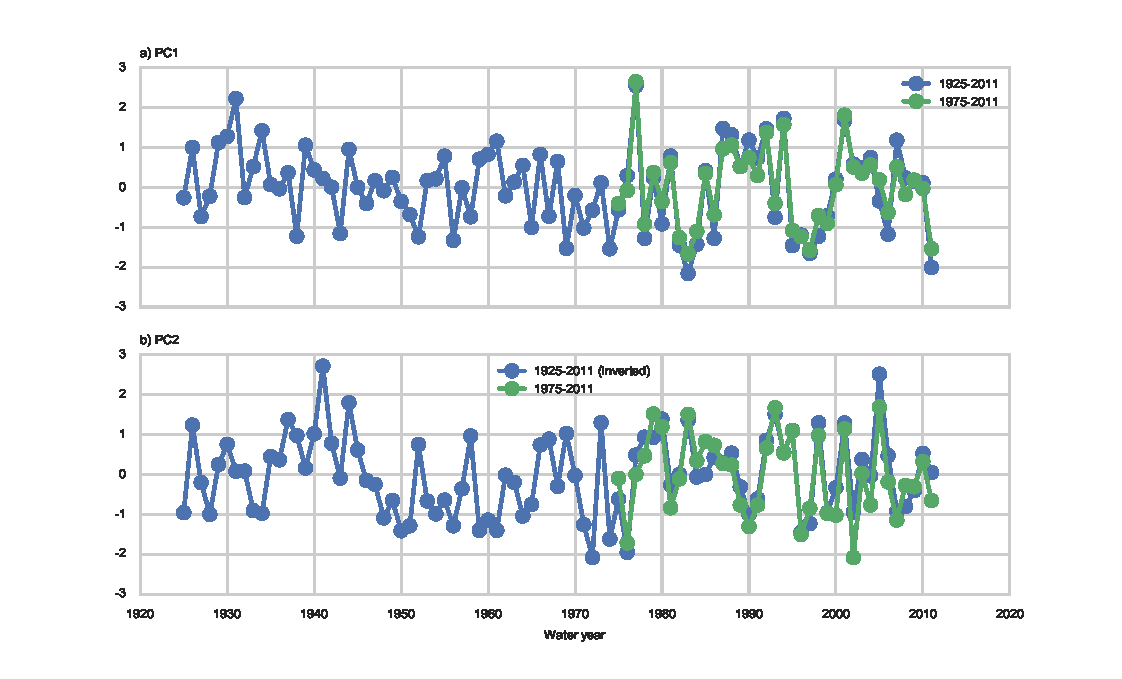
\includegraphics[width=190mm]{p1figures/s4.pdf}}
\caption{Time series of leading streamflow principal components a) PC1 and b) PC2 from HCDN in WY1925 - 2011 and WY1975 - 2011. The leading principal components from the two periods are similar, suggesting a that we have a robust pattern, at least through to the early quarter of the century.}
\label{sfig:pctimeseries}
\end{figure}

\begin{figure}[ht]
\centering
\centerline{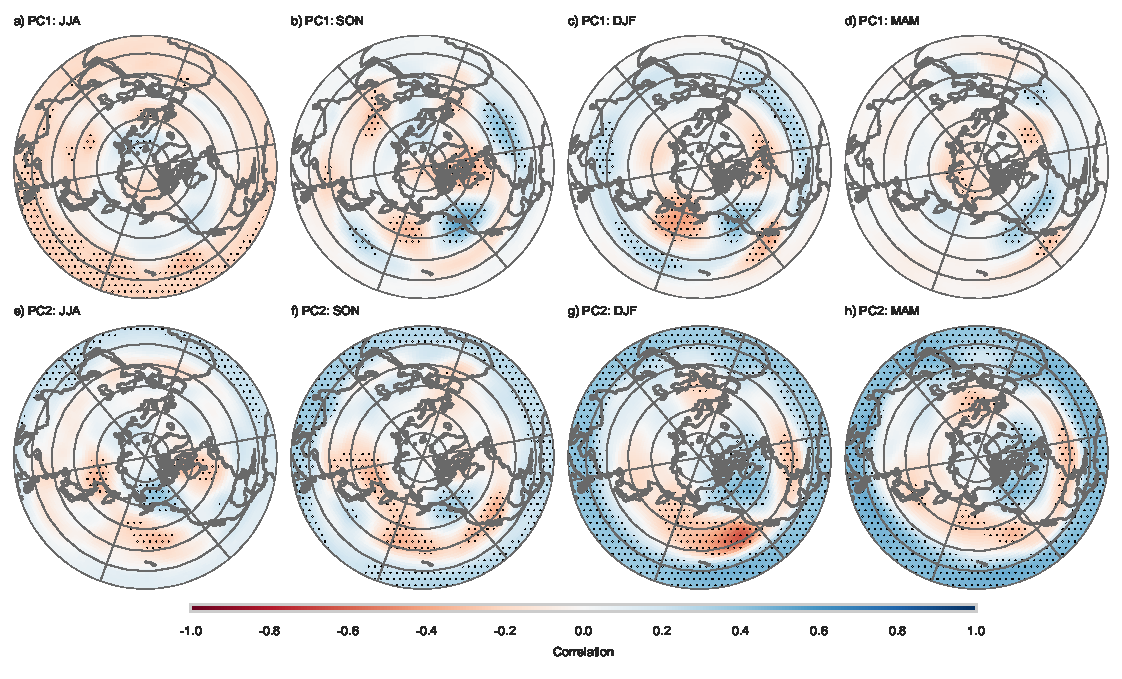
\includegraphics[width=190mm]{p1figures/s5.pdf}}
\caption{Seasonal point correlation maps as in Figure 2, but using streamflow PCs and 500 mb geopotential height field data from WY1925 - 2011. Note that PC2 has been inverted to match the sign in the WY1975 modes.}
\label{sfig:corrhgt}
\end{figure}

\begin{figure}[ht]
\centering
\centerline{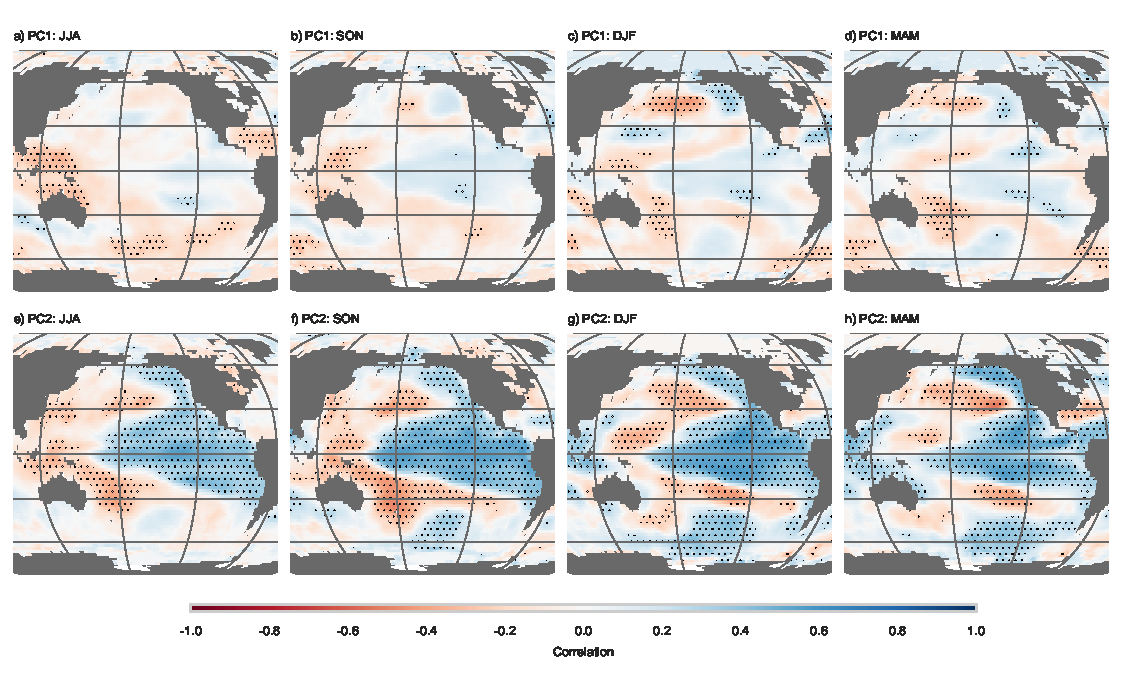
\includegraphics[width=190mm]{p1figures/s6.pdf}}
\caption{Seasonal point correlations as in Figure 4, but using streamflow PCs and ERSST data from WY1925 - 2011. Note that PC2 has been inverted to match the sign in the WY1975 modes.}
\label{sfig:corrsst}
\end{figure}

\begin{figure}[ht]
\centering
\centerline{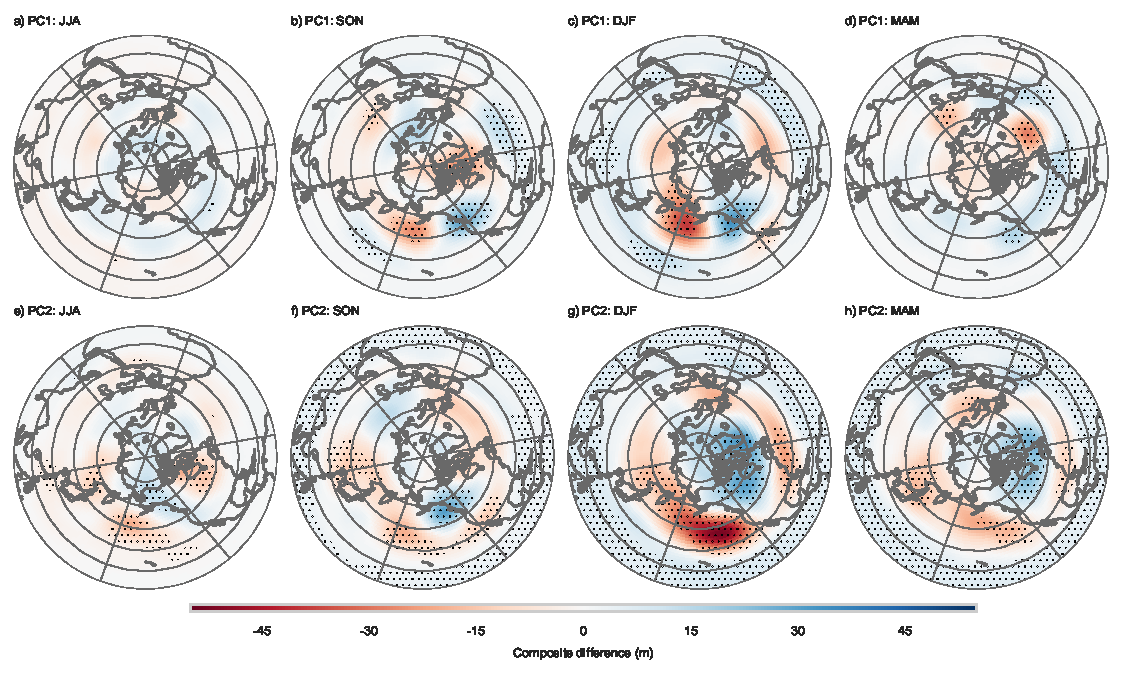
\includegraphics[width=190mm]{p1figures/s7.pdf}}
\caption{Seasonal composite maps as in Figure 3, but using streamflow PCs and 500 mb geopotential height field data from WY1925 - 2011. Note that PC2 has been inverted to match the sign in the WY1975 modes.}
\label{sfig:comphgt}
\end{figure}

\begin{figure}[ht]
\centering
\centerline{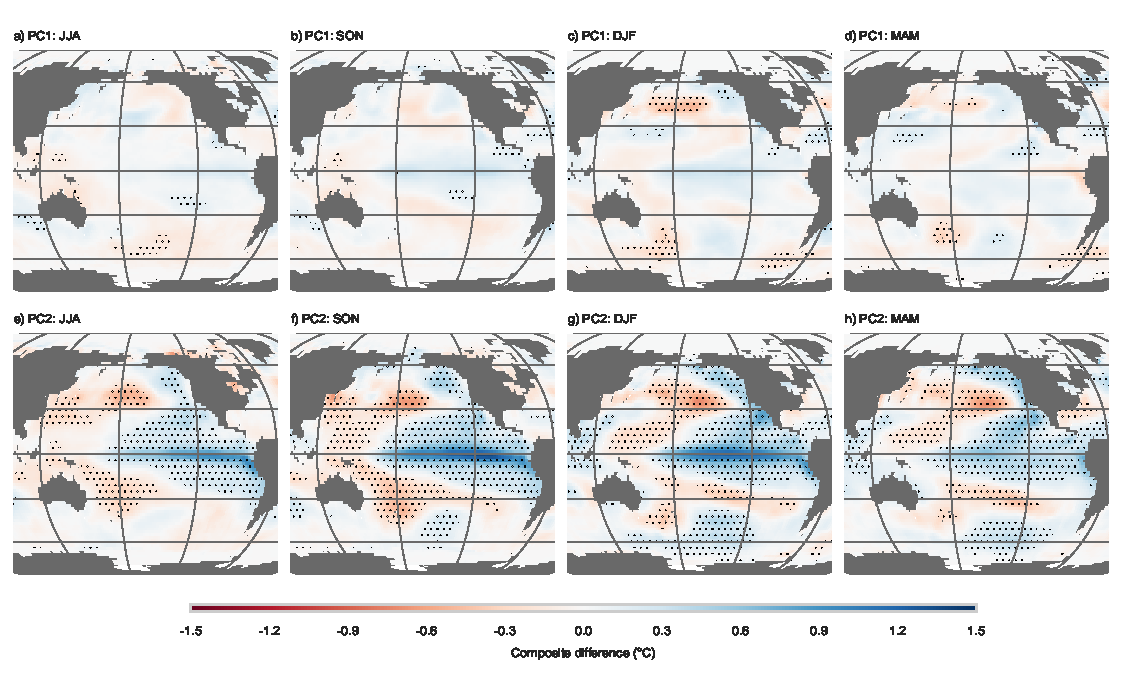
\includegraphics[width=190mm]{p1figures/s8.pdf}}
\caption{Seasonal composite maps as in Figure 5, but using streamflow PCs and ERSST data from WY1925 - 2011. Note that PC2 has been inverted to match the sign in the WY1975 modes.}
\label{sfig:compsst}
\end{figure}


\chapter{The importance of coastal Pacific ridge and Aleutian low position and intensity for widespread interannual anomalies in western US streamflow}

\section{Abstract}

Widespread drought can have a significant impact on interannual western US streamflow. The causal mechanism for these events are often discussed in terms of shifts to the winter storm track, relating to changes in the seasonal position and intensity of the Aleutian low and persistent atmospheric ridges along the North American Pacific coast. This study applies an object-tracking framework, using watershed segmentation algorithms, to track variations in the wintertime position and intensity of these semi-permanent atmosphere features. We compare these characteristics with annual streamflow anomalies across the western US from 1930 - 2006. Coastal ridges position and intensity exhibits considerably more variability relative to the Aleutian low. We find that widespread streamflow anomalies are most strongly linked to changes wintertime coastal ridge intensity, while latitudinal position is more strongly associated with teleconnections from the tropical Pacific. The Aleutian low centers at higher latitude associates with widespread streamflow anomalies, but this association is largely focused in the US Northern Rockies and Pacific Northwest. These results have implications for multi-basin water management in the Western US, now and in the future, as Pacific coast atmosphere circulation has considerable uncertainty in climate change projections.

\section{Introduction}

In the western United States (US), human and ecosystem development has been shaped by competing and increasing demands for water resources. Widespread drought can have a dramatic impact on the western US. Streamflow anomalies affecting multiple river basins can be especially challenging for regions with water supply needs met through surface water from multiple river basins.  Spatial coherence and widespread anomalies are a prominent characteristic  of interannual western US streamflow \citep{2cayan_influence_1989, 2lins_regional_1997}. This characteristic reflects the common drivers of hydroclimatic variability influencing river basins that are otherwise hydrologically independent. Through the last century, widespread interannual streamflow anomalies in the western US have been driven by both internal atmospheric dynamics and Pacific sea surface temperatures (SSTs), noteably El Ni\~{n}o-Southern Oscillation-related (ENSO) teleconnections \citep{2cayan_influence_1989, 2redmond_surface_1991, 2cayan_enso_1999}. These influence streamflow in multiple river basins by steering mid-latitude wave trains and cool-season moisture delivery. The position and intensity of seasonally persistent atmospheric ridges near the North American Pacific coast and the semi-permanent Aleutian low in the west-central North Pacific are key components of this circulation system. However, it remains unclear how consistently changes in the position and intensity of these individual features relate to interannual streamflow variability in the western US, at a large spatial scale. Widespread streamflow anomalies in the western US are rarely studied on larger, multi-basin scales, in part because streamflow-oriented climate studies generally focus on one or two river basins that share common administrative significance, and in part because this characteristic is not reliably driven by an established source of persistent climate variability that can be exploited for operational forecasting.

Prior hydroclimate studies have investigated the strong inter-basin correlation and covariability of streamflow as a response to seasonal shifts in the position and intensity of the Aleutian low \citep{2cayan_influence_1989}. The Aleutian low relates to the movement of mid-latitude cyclones through the central and western North Pacific. Recent hydroclimate and drought-oriented research has focused on the position and intensity of persistent atmospheric pressure ridges near the North American Pacific coast \citep{2cook_worst_2014, 2seager_causes_2014, 2wise_persistence_2014, 2seager_causes_2015, 2swain_tale_2015, 2choi_uncertainty_2016, 2wise_five_2016}. Both the Aleutian Low and the coast ridge are embedded components of a larger standing atmospheric wave pattern that forms from the combined influence of general zonal atmospheric flow, topography, interaction with transient eddies, and diabatic heating. However, hydroclimate and drought studies loosely discuss the Aleutian low and seasonally persistent ridges as separate entities that can ``block'' or ``fork'' incoming Pacific storm tracks \citep[e.g., ][]{2cayan_influence_1989, 2sheppard_climate_2002}. Relationships between streamflow and seasonal mid-latitude atmospheric circulation have been established using Eulerian methods, such as point-correlation maps with atmospheric pressure, or climate indices derived from fixed-points in space and/or prominent modes of climate variability \citep[e.g., ][]{2wallace_teleconnections_1981}. These are undoubtedly powerful approaches, however, beyond case-by-case research for a handful of individual drought events, hydroclimate studies have not explicitly tracked the seasonal position and intensity of the Aleutian low and coastal ridges with respect to streamflow anomalies. The form and stregth of the relationship between these semi-stationary atmospheric features and interannual streamflow variability in the western US have not yet been investigated.

This issue has important implications for western US water supplies and water management. Quantifying the relationship between widespread streamflow anomalies and the position and intensity of influential, persistent atmospheric features can improve our understanding of the climatic condtions surrounding severe and widespread drought events recorded in the past. Additionally, future anthropogenic climate change is projected to alter mid-latitude storm tracks and stationary atmospheric waves in the North Pacific. There is considerable uncertainty surrounding these projections and the variability of future western US water supplies \citep{2dettinger_western_2015, 2langenbrunner_patterns_2015, 2choi_uncertainty_2016}. Understanding how widespread streamflow anomalies relate to variability in the position and intensity of these waves can help us begin to understand how future climate change may affect interannual streamflow variability across western US rivers.

In this paper, we investigate the Aleutian low and persistent coastal Pacific ridges and their influence on western US interannual streamflow through cool-season moisture delivery. Our approach involves a novel application of segmentation algorithms to search for and measure semi-permanent atmospheric features as cohesive objects on a geopotential height surface, akin to the object-tracking framework used to generate storm track and cyclone records \citep[e.g., ][]{2hodges_general_1994, 2hoskins_new_2002}. Our goal is to explore how variability in the cool-season position and intensity of these atmospheric features relates to interannual streamflow variability. Specifically, we are guided by the following question: Is multi-basin variability in interannual western US streamflow more strongly relate to the position and intensity of the Aleutian low or coastal ridges? And more broadly, how does streamflow variability related to these two features?

We begin by characterizing western US streamflow series and climate data used to to explore these relationships. Next, we describe our analysis and use of segmentation algorithms to identify and follow persistent atmospheric features. We analyze the variability in the position and intensity of the Aleutian low and coastal atmospheric ridge through the last century. Finally, we discuss how changes in the seasonal position and intensity of these persistent features appear to relate to streamflow variability across the western US.

\section{Data}

\subsection{Western US streamflow series}

For this study, we used five water-year (October-September) streamflow series extending from 1930 to 2006 (Figure \ref{fig_samplemap}). These series are estimated natural flows, for which the effects of anthropogenic influences such as reservoir operations or depletions from agriculture have been accounted. These five streamflow records were selected for their length and spatial coverage across western US basins that have significance for water management and policy. Each of these records is from a hydrologically independent river basin, but they share variability (Figure \ref{fig_river_cluster}) that reflects common climate influences. 

The five streamflow records include the ``Colorado River at Lees Ferry, AZ'', ``Columbia River at The Dalles, OR'', ``Missouri River at Toston, MT'', ``Sacramento Four Rivers Index'', and the ``South Platte River at South Platte, CO''. Information from these gages is summarized in Table \ref{table:series}. Each of this gages is important to water supplies across the western US.

The streamflow series were standardized to account for the different moments of streamflow distributions between the different river basins. Each streamflow series was standardized through a cumulative distribution function using maximum likelihood estimates of gamma distribution shape and scale parameters. This standardization is applied to streamflow like the standardized precipitation index \citep{2mckee_relationship_1993} is applied to precipitation.


\subsection{Climate data}

We used monthly reanalysis geopotential height fields averaged into seasonal December-February (DJF) fields from 1930 to 2006. These geopotential height fields are from the NOAA-CIRES Twentieth Century Reanalysis Version 2c (TCR) \citep{2compo_twentieth_2011}. This product has a 2$^{\circ}$ by 2$^{\circ}$ global grid. The Aleutian low, and persistent coastal ridges were identified at the 1000 mb and 500 mb level, respectively. The 500 mb level was used in the search for coastal ridges because this level does not intersect -with the North American Cordillera. The 1000 mb level is used for the Aleutian low because this feature is frequently measured near the surface. We focused on DJF because it is a season with relatively well-formed troughs and ridges that are easily identified on geopotential height maps. DJF geopotential height anomalies relating to Pacific coastal ridges and the Aleutian low are significantly correlated with widespread streamflow anomalies \citep{2malevich_pacific_2016}.

We used SST and standardized precipitation index (SPI) fields to investigate streamflow PCs. SST fields were averaged into DJF seasons from monthly NOAA Extended Reconstructed Sea Surface Temperature V4 (ERSST) \citep{2huang_extended_2014, 2liu_extended_2014, 2huang_further_2015}. The linear trend was removed from the SST fields, prior to analysis. Three-month SPI was calculated from Climate Research Unit Time Series (CRU TS) 3.21 global land surface precipitation fields (1949 - 2012) \citep{2oloughlin_climate_2012, 2cisl_rda_ds2980}.

\section{Methods}


\subsection{Measuring the position and intensity of the winter coastal ridge  and the Aleutian low}

Traditionally, the position of major semi-permanent air masses, like the Aleutian low, have been identified by finding the minima or maxima within a bounding box over a specified area on a pressure or geopotential height field \citep[e.g., ][]{2overland_decadal_1999}. However, this method can be problematic when used to find to seasonally persistent coastal Pacific ridge. The coastal ridge is not always a single coherent or persistent feature as the semi-permanent Aleutian low. As a consequence, the pressure or geopotential height maxima in a specified bounding box over the eastern North Pacific - often a ridge associated with strong Alaskan blocking \citep{2carrera_downstream_2004} - may not always correspond to the ridge immediately influencing atmospheric flow into the western US. Additionally, storm tracks can be disrupted by more than one coastal ridge in the same season. This is often the case when strong subtropical highs near the southern California coast persists through the fall and winter. We therefore approached this problem by treating the search for the potentially influential ridge and troughs as a segmentation problem.
% * <malevich@email.arizona.edu> 2017-01-04T20:23:22.875Z:
%
% > As a consequence, the pressure or geopotential height maxima in a specified bounding box over the eastern North Pacific - often a ridge associated with strong Alaskan blocking \citep{carrera_downstream_2004} - may not always correspond to the ridge immediately influencing atmospheric flow into the western US
%
% Might want to expand and add citations to this. See Carrera 2004.
%
% ^.

Segmentation algorithms are novel in this application but are commonly used in image processing and computer vision \citep{2digabel_iterative_1978, 2vincent_watersheds_1991, 2dougherty_morphological_1993, 2cousty_watershed_2009}. Specifically, we use marker-watershed segmentation, which is a transformation often used to detect and differentiate independent objects or surfaces that might overlap or obscure one another in an image (Figure \ref{fig_cat_segmentation}). The algorithm is a two-step process carried out on a geopotential height field (Figure \ref{fig_watershed_explaination}a). It begins like many object-tracking algorithms used for storm-track analysis \citep[e.g., ][]{2lambert_cyclone_1988, 2murray_numerical_1991, 2hodges_general_1994, 2hoskins_new_2002}: when searching for persistent troughs, we first use the geopotential height zonal-anomaly field to identify local minima, our ``markers'', while for ridges, we use the local maxima to identify markers. These markers give the center position and intensity for each ridge or trough (Figure \ref{fig_watershed_explaination}b). For the second step, imagine that we fill the zonal-anomaly field with water from these markers as though flooding a topographic surface. The water level rises until it meets water from different markers. At this point, the edges of each flooded area delimit segments based on the gradient of the underlying zonal-anomaly surface. We use the segments created by this algorithm as a simplistic, though objective, non-parametric, and computationally inexpensive way to parse the relative spatial ``influence'' of mid-latitude ridges and troughs. The dependence on geopotential height fields is also convenient because it is generally among most reliable variables in model and reanalysis datasets \citep{2kalnay_ncep/ncar_1996}. We use the segment information as a query, selecting only ridge segments or trough segments that influence a target point or area in space by finding the ridge or trough segment that overlaps with the target position (Figure \ref{fig_watershed_explaination}c). This allows us to create a time series of the center latitude, longitude, and intensity of the persistent coastal ridge and the Aleutian low. We also used this information to isolate the full surface of the ridge or trough anomaly contained within the segment.

Specifically for this study, we used the watershed segmentation algorithm implemented in the scikit-image library for Python (available online at \url{http://scikit-image.org/}). For further implementation details, example code that describes a watershed segmentation problem for the December 1976 ridge is available in Supplemental Information.

The target points for identifying the coastal ridge and the Aleutian low were 48$^{\circ}$N, 120$^{\circ}$W and 50.0$^{\circ}$N 176$^{\circ}$E, respectively. These points are the average winter zonal-anomaly maxima and minima for the northmost ridge along the US-Pacific coast and Aleutian low, from 1930 to 2006. These points closely correspond with positions in DJF 500 mb geopotential height that are significantly correlated with multi-basin streamflow anomalies (Figure \ref{fig_streamflow_pc_hgt}). We confirmed that the segmentation method produced sensible solutions by visually checking the solution for each winter of the analysis.


\subsection{Identifying widespread streamflow anomalies}

We use PCA as the basis for identifying streamflow anomaly patterns and time series. PCA was based on singular value decomposition of the standardized streamflow series' covariance matrix \citep{2wilks_statistical_2006, 2dawson_eofs:_2016}. We identified two leading streamflow PCs and confirmed that they were well-separated from their siblings \citep{2north_sampling_1982}. Streamflow PC1 and PC2 account for 56\% and 24\% of variability in the streamflow data, respectively. As shown in prior studies, PC1 generally represents nearly west-wide high or low interannual streamflow anomalies associated with North Pacific mid-latitude atmosphere wave trains, while PC2 is a north-south, dipole covariability in streamflow that loosely reflects a response to ENSO teleconnections \citep{2malevich_pacific_2016}. Similar patterns are shown in the stream empirical orthogonal functions (EOFs), mapped as covariance of PC1 and PC2 on the standardized streamflow series (Figure \ref{fig_streamflow_eofs}). We confirmed these relationships with point-correlation maps of streamflow PC1 and PC2 on SST fields (Figure \ref{fig_streamflow_pc_sst}) and 500 mb geopotential heights (Figure \ref{fig_streamflow_pc_hgt}). We also confirmed that our leading streamflow PCs were not strongly bias by the period of analysis, nor streamflow series selection, by correlating each PC with the 1925 - 2011 and 1975 - 2011 PCs identified from a larger western US streamflow network in \citet{2malevich_pacific_2016}. Our streamflow PCs are similar to the ``Far West'' and ``Western Opposition'' patterns in the US-wide PCA of river discharge from \citet{2lins_regional_1997}, suggesting that our PCs are reasonably unbiased by our western US-focused spatial domain. Composite analysis confirmed that our streamflow PCs generally correspond with cool-season precipitation (Figure \ref{fig_spi_composite}).

We defined ``widespread streamflow anomalies'' as the first principal component (PC1) of standardized western US water year streamflow through the half last century. We differentiate this from second principal component (PC2), which we will refer to as ``dipole variability'' in discussion, as this is generally linked with a linear teleconnection response in the western hydroclimate to ENSO variability.

\subsection{Aleutian low and ridge associations with streamflow}

We used correlation statistics and scatter plots to compare Aleutian low and coastal ridge center latitude, longitude, and intensity with widespread interannual streamflow anomalies (streamflow PC1). We then examined the relationship with individual streamflow series using similar methods. We note correlations as statistically significant following a two-sided $t$-test ($\alpha = 0.05$).

\section{Results \& discussion}

\subsection{Position and intensity of the winter coastal ridge and the Aleutian low}

Over the 77 years of our analysis (1930 - 2006), the center position of the winter Aleutian low is largely restricted to longitudinal movement within the North Pacific (Figure \ref{fig_aleutian_stats}a). The Aleutian low center mean latitude is 49.4$^{\circ}$N with an inner quartile range between 48.0$^{\circ}$N and 50.0$^{\circ}$N (Figure \ref{fig_aleutian_stats}b). The lowest latitude observed for the Aleutian low center is 42.0$^{\circ}$N in water year 1963 while the highest is 54.0$^{\circ}$N in water year 1931. The Aleutian low center mean longitude is 177.5$^{\circ}$E with an inner quartile range between 168.0$^{\circ}$E and 174.0$^{\circ}$W (Figure \ref{fig_aleutian_stats}c). The west-most observed Aleutian low center is 152.0$^{\circ}$E in water year 1956 while the east-most is 148.0$^{\circ}$W in water year 1998. The average eddy intensity of the Aleutian low center is -152.7 m with an inner quartile range between -171.7 m and -135.0 m (Figure \ref{fig_aleutian_stats}d). The weakest Aleutian low intensity is -94.2 m in water year 1971. The deepest Aleutian low intensity was -217.7 m in water year 1931.

We generally find the coastal ridge near the Pacific Northwest, though the distribution extends up and down the North American coast (Figure \ref{fig_ridge_stats}a). The ridge center mean latitude is 50.0$^{\circ}$N with an inner quartile range between 46.0$^{\circ}$N and 52.0$^{\circ}$N (Figure \ref{fig_ridge_stats}b). The lowest latitude observed for the ridge center was 38.0$^{\circ}$N in water year 1965 while the highest was 66.0$^{\circ}$N in water year 1949. The ridge center mean longitude is 125.3$^{\circ}$W with an inner quartile range between 130.0$^{\circ}$W and 120.0$^{\circ}$W (Figure \ref{fig_ridge_stats}c). The west-most observed ridge center was 168.0$^{\circ}$W in water year 1950 while the east-most was 110.0$^{\circ}$W in water year 1969. The average eddy intensity of the coastal ridge center is 135.4 m with an inner quartile range between 118.8 m and 157.7 m (Figure \ref{fig_ridge_stats}d). The lowest recorded ridge intensity was 40.1 m in water year 1932. The most intense ridge was 250.8 m in water year 1977 - an extreme outlier  that is beyond 1.5 standard deviations from the Ridge intensity mean (Figure \ref{fig_ridge_stats}d). This outlier is associated with the significant 1977 drought, which saw intense, dry streamflow anomalies across much of the Western US. Relative to the Aleutian low characteristics, the coastal ridge characteristics are considerably more sparse, with strong outlying values. 

We examine the robustness of variability in the ridge surface by isolating the surfaces of the coastal ridge anomalies from each of the influential ridge segments. EOFs of these ridge surfaces shows spatial clusters (Figure \ref{fig_ridge_eofs}) that correspond with clustering  in coastal ridge centers (Figure \ref{fig_ridge_clustermap}). With the mean removed from the ridge surfaces, there are three leading EOFs. The first EOF (accounting for 33\% of variability) shows a strengthening of the ridge anomaly, focused in the Pacific Northwest US (Figure \ref{fig_ridge_eofs}a). The second EOF (26\% of variability) highlights ridge anomalies focused just off the Pacific coast of the North America, north of 40$^{\circ}$N latitude (Figure \ref{fig_ridge_eofs}b). The third EOF (16\% of variability) reflects an intensification of ridge anomalies near 60$^{\circ}$N latitude, over Alaska (Figure \ref{fig_ridge_eofs}b). A $k$-means clustering of ridge centers based on center latitude and longitude produces similar groupings (Figure \ref{fig_ridge_clustermap}). We repeat this PCA/EOF analysis using the coastal ridge identified in the first and later half of the TCR, which extends from water year 1852 to 2013. These ridge surface EOFs largely reflect the same type of clustering with little change, though the leading EOFs swap their order. This then suggests that, despite the sparely distributed ridge center characteristics and extreme values, the leading modes of variability in the ridge surfaces are generally robust through the last century, at least in so far as this is represented in the TCR.

Because the Aleutian low and coastal ridge are neighboring features of a standing, mid-latitude atmospheric wave, we expect some collinearities between these atmosphere feature characteristics. As expected, in a given winter, we find that a deepening of the Aleutian low coincides with an intensification of the coastal ridge and \textit{vice versa} ($r = -0.53$, $p < 0.01)$. We also find that a northward (southward) shift in the center latitude of the Aleutian low is generally associated with a northward (southward) shift in the coastal ridge center ($r = 0.24$, $p = 0.03$).

In summary, over our 77 year analysis, we find more spatial variability in wintertime coastal ridge relative to the Aleutian low. Ridge characteristics also have noteworthy outliers. An important example is the extreme ridge intensity in 1977, which corresponds with one of the most significant and widespread drought in the western US streamflow record. Despite this variability in the coastal ridge, the leading EOFs of ridge geopotential height surfaces appear reasonably robust the late 20th and 21st century, as represented in the TCR. We find the expected covariability between the center position and intensity of the coastal ridge and the Aleutian low: a deepening of the Aleutian low is generally matched with a strengthening of the coastal ridge; a northward shift in the coastal ridge center is generally matched by a northward shift in the Aleutian low center.

\subsection{Aleutian low and ridge characteristics in relation to western US streamflow anomalies}

With the Aleutian low, we find a negative linear, though statistically insignificant relationship between Aleutian low intensity and widespread streamflow anomalies ($r = 0.18$, $p = 0.11$) where a deepened (weakened) Aleutian low corresponds with widespread dry (wet) streamflow anomalies (Figure \ref{fig_feature_pc1_scatter}). The center longitude of the Aleutian low has a non-significant linear relationship with widespread streamflow anomalies. In contrast to this, however, we find the Aleutian low center latitude to have a significant, though moderate, positive linear relationship with widespread streamflow anomalies, linking Aleutian low centers at higher (lower) latitude with widespread dry (wet) streamflow anomalies ($r = -0.27$, $p = 0.02$). This is not surprising as streamflow point correlation with 500 mb geopotential heights show locally significant correlations at higher latitudes in the North Pacific, corresponding with strong ridge-like anomalies in the Pacific Northwest and widespread low flow anomalies (Figure \ref{fig_streamflow_pc_hgt}). Interestingly though, we find insignificant correlations with the Aleutian low center intensity despite the correlations in Figure \ref{fig_streamflow_pc_hgt}, and elsewhere in streamflow-climate research \citep[e.g., ][]{2cayan_influence_1989, 2lins_regional_1997, 2malevich_pacific_2016}. The strength and position of the Aleutian low has been discussed as a key influence on widespread streamflow anomalies in past literature \citep[e.g., ][]{2cayan_influence_1989, 2lins_regional_1997}, yet here the only statistically significant correlation we find is with the Aleutian low center latitude.

For the winter coastal ridge, the strongest relationship is between the intensity of coastal ridges and widespread streamflow anomalies ($r = -0.33$, $p \ll 0.01$), associating increased (decreased) ridge intensity with widespread dry (wet) anomalies (Figure \ref{fig_feature_pc1_scatter}). A negligible correlation with widespread streamflow anomalies is found with the center latitude of the winter coastal ridge ($r = -0.09$, $p = 0.46$). The relationship between the central longitude of winter coastal ridge and widespread streamflow anomalies is also negligible ($r = 0.03$, $p = 0.80$). The significant relationship we see here is with ridge intensity, which is more strongly correlated to widespread streamflow anomalies than any of the Aleutian low characteristics. This suggests that the seasonally persistent coastal ridge generally have a stronger linear relationship with widespread streamflow anomalies than the Aleutian low. Additionally, we might expect a link between a blocking ridge position and widespread streamflow anomalies. However, these correlations give no statistically significant association between ridge center position and widespread streamflow anomalies.

We examine this further by checking these ridge characteristics against the ENSO-linked dipole variability in streamflow. The western US hydroclimate response to the ENSO teleconnection greatly depends on north-south positional shifts in mid-latitude atmosphere circulation, so we expect to find a significant linear association between coastal ridge position characteristics and the dipole variability of western US streamflow (streamflow PC2). We find coastal ridge intensity ($r = 0.24$, $p = 0.04$) and center latitude ($r = 0.29$ with $p = 0.01$) both have a statistically significant positive correlation with streamflow dipole variability, meaning strong (weak) ridge centers at a higher (lower) latitude associate with wet, El Ni\~{n}o-like (dry, La Ni\~{n}a) streamflow anomalies in the south western US and dry (wet) anomalies in the north western US. These correlations reflect the relationships we would expect to find in these variables.

In relation to the correlations discussed above, ENSO-related variability in streamflow (streamflow PC2) appears more strongly related with latitudinal shifts in the coastal ridge. Ridge intensity, on the other hand, is more strongly associated with widespread variability in streamflow (streamflow PC1). The association between ridge surface PCs and streamflow PCs gives further evidence to support this: widespread streamflow variability (streamflow PC1) is most strongly correlated with intensification of the widespread ridge anomalies centered over the Pacific Northwest (ridge PC1, Figure \ref{fig_ridge_eofs}a) ($r = -0.29$). ENSO-related streamflow variability (streamflow PC2) is most strongly correlated with intensification of ridge anomalies further up the North American Pacific coast (ridge PC3, Figure \ref{fig_ridge_eofs}c) ($r = -0.34$), corresponding with the north-south dipole in the western US hydroclimate.


\subsection{Poor linear association between ridge center position and widespread streamflow anomalies}

We do not find a significant correlation between widespread streamflow anomalies and the center latitude and longitude of the coastal ridge.  In order to determine if this result is due to a overly simple approach to defining ridge latitude and longitude, we performed several additional analyses.  We divided the individual streamflow series into discrete groups determined by position-based clusters of the wintertime coastal ridge (Figure \ref{fig_ridge_clustermap}). The ridge position clusters do not correspond with distinguishable streamflow distributions (Figure \ref{fig_streamflow_ridgecluster_violins}). This may, in part, be due to the limited number of realizations in several of the ridge position clusters. An alternative approach is to map the position of the wintertime ridge for the five water years with the wettest and driest streamflow anomalies (Figure \ref{fig_ridge_streamflow_position}). These maps show that ridge position in dry streamflow anomaly years is often, but not always, adjacent to the catchment of each river basin. During wet anomaly years, however, there is more variability in the placement of the ridge and it is common for wet and dry year ridge placement to be indistinguishable. These maps, and our previous results, suggest that seasonal ridge center placement through the last century has not been as important as ridge intensity for widespread streamflow anomalies. Clearer relationships with ridge position could emerge with a larger sample size or in an analysis of synoptic rather than seasonal atmospheric variability.

We generally find that years with the poorest correspondence between streamflow anomalies and ridge center intensity are not explained by wintertime ridge placement, but by influences in other seasons such as the preceding fall or spring. One example of this is water year 2002, which has dry anomalies in many of our streamflow series and can be clearly seen in streamflow PC1 (highlighted with 1977 for contrast in Figure \ref{fig_feature_pc1_scatter}). These streamflow anomalies are  considerably drier than we might expect given the weaker intensity of the DJF ridge. However, we find that this 2002 observation appears better explained by the above average ridge intensity in the spring of that water year and strong drought conditions during the summer. We focus on DJF in this study because this is a season with well-formed semi-permanent atmosphere features with generally higher significant correlations relative to other seasons. But, influence from other seasons obviously can be of practical significance to water year streamflow values.


\subsection{Relationships with individual river basins}

Here we briefly describe relationships with natural streamflow estimate series from individual rivers. This gives us an opportunity to discussed how the relationships described in the previous section break down within the western US.% As in the previous section, we use correlation statistics and scatter plots. We begin the discussion with river basins in the northern Rockies and Pacific Northwest and move to southwest river basins and basins in the interior Rockies and eastern Front Range.
 The correlations discussed below are summarized in Table \ref{table:corrs}.

\subsubsection{Columbia River}

We find that low streamflow values on the Columbia River are favored by a deepened Aleutian low at the higher end of its latitudinal range (Table \ref{table:corrs}). For the coastal ridge, low Columbia River flows associate with an intensification of the ridge, especially at higher latitudes. Columbia River flow has a negligible relationships with coastal ridge longitude.

Our Columbia River correlations underline the basin's relatively strong sensitivity to North Pacific climate variability. The Columbia series has significant correlations with both Aleutian low center intensity and latitude. Additionally, of all the river basins in this study, the Columbia River series has the strongest correlation with coastal ridge intensity ($r = -0.39$). Given these strong relationships and the river basin's position in the Pacific Northwest, this result was not unexpected.

\subsubsection{Upper Missouri River}

The Upper Missouri River streamflow series coincide with deepened Aleutian low in the upper latitudes (Table \ref{table:corrs}). Dry streamflow anomalies in the Upper Missouri also associate with an intensification of the coastal ridge, generally at higher latitudes. Of the streamflow series we examined, the Missouri series is most strongly correlated with the latitude of ridge centers. The correlation with ridge center longitude was negligible.

Much like the Columbia River streamflow series, this analysis shows that the Upper Missouri series is relatively sensitive to North Pacific atmosphere circulation. Streamflow in both basins is significantly correlation with Aleutian low latitude. These are the only two of the five rivers where this pattern is observed. 

\subsubsection{Sacramento River}

The Sacramento River flow is not significantly correlated with any aspect of the Aleutian low (intensity, longitude, or latitude; Table \ref{table:corrs}). In contrast, flow is significantly correlated with ridge intensity and longitude.  A strong, westerly positioned ridge intensity favors low Sacramento River flow ($r = -0.33$, $p \ll 0.01$), and the reverse for high flow years. Much like with the Columbia basin further to the north, we see a relatively strong correlation with coastal ridge intensity, as might be  expected, but there is no significant correlation with coastal ridge center latitude despite the Sacramento basin's coastal position.

\subsubsection{Upper Colorado and South Platte River}

Similar to the Sacramento River, Colorado River streamflow has no statistically significant correlations with Aleutian low intensity, longitude, and latitude (Table \ref{table:corrs}). However, coastal ridge latitude, longitude, and intensity also all have statistically insignificant correlations with our Colorado River series. The strongest relationship shown in our correlations is with coastal ridge intensity, which is considerably weakened ($r = -0.17$, $p = 0.13$) relative to basins further west and north (the Columbia, Missouri, and Sacramento). This lack of association with the three measures of the Aleutian low and coastal ridge is also evident in South Platte River flow (Table \ref{table:corrs}).

In summary, we find that the intensity of the DJF coastal ridge has the strongest linear relationship with widespread streamflow anomalies in the western US. This influence is also stronger and significant in more river basins than any of our other coastal ridge and Aleutian low characteristics. The latitude of the Aleutian low is significantly correlated with widespread anomalies, but correlations with individual streamflow basins shows that this significant influence is confined to the north-most river basins. Influence from the ridge and the Aleutian low greatly diminishes towards the eastern-interior Rockies, likely reflecting the more complicated influences on cool-season precipitation deliver \citep[e.g., ][]{2changnon_hydroclimatic_1991}


% [here it would be good to comment on this; why this result? also some of the more general comparison comments from the other basin resutls, as I've indicated. I see yo have a "synopsis section below (e) , which seems a little odd. I'd move that, along with these more general comments to the conclusions ] [I think Table 2 is more useful than figs 14 and 15; I'd consider deleting them unless there are aspects that aren't conveyed in the table]

% [I WOULD DELETE THE REST OF THIS PARAGRAPH, AND CONSIDER MOVING ANYTHING RELEVANT TO A COMPARISON W/ OTHER BASINS TO THE END OF THIS SECTION The Columbia streamflow series does not a have significant correlation with ridge latitude. Granted the correlation with ridge latitude ($r = -0.19$) is among the strongest of the streamflow series. But, against our expectations, this is evidently not a strong enough linear relationship for statistical significance. We suspected that a uniquely non-linear relationship may exist relating to a change in influence from ridge center latitudes at north and south extremes, but did not find significant evidence for this kind of relationship in this streamflow series.]

%  Much like the majority of streamflow series in our study, we find a statistically significant relationship with the intensity of coastal ridges.] ] In addition, the Missouri River flow has the strongest correlation with the latitude of the coastal ridge center of all the basins.  This may reflect the relationship between ridge latitude, meridional atmospheric flow, and jet stream exit region placement in the northwestern Rockies.


\section{Conclusions}


Our analysis shows that, within the last century (1930 - 2006), widespread interannual streamflow anomalies in the western US have been more strongly associated with winter variability in the coastal Pacific Northwest ridge than the Aleutian low. Specifically, we show that widespread streamflow anomalies more strongly correlate with coastal ridge intensity and ridge characteristics than Aleutian low characteristics. This has implications for the future of multi-basin water management in the western US. We show that widespread streamflow anomalies have a relatively strong association with eastern North Pacific atmospheric circulation. Widespread streamflow anomalies also have a significant relationship with the Aleutian low, particularly its latitudinal position, but this influence is largely confined to river basins in the Pacific Northwest and North Rockies. Influence from the ridge and the Aleutian low greatly diminishes towards the eastern-interior Rockies.

Our measurements of these semi-permanent atmosphere features are based on a simple object-tracking approach that incorporates novel use of segmentation algorithms. Through the last century, the coastal ridge has exhibited considerable variability relative to the Aleutian low. The 1977 drought - for example - is  outlying observation in ridge intensity. In spite of this, we find that the leading modes of variability within the coastal ridge are reasonably robust through the last century. We find that the coastal ridge variability in the eastern North Pacific has a stronger direct relationship with widespread interannual streamflow anomalies than Aleutian low variability in the western North Pacific. Future climate projections suggest there may be a poleward-shift in the midlatitude storm track with an expansion of the Hadley cells \citep[e.g., ][]{2frierson_width_2007, 2scheff_twenty-first-century_2012, 2neelin_california_2013, 2chang_significant_2015, 2langenbrunner_patterns_2015, 2choi_uncertainty_2016}. There is a great deal of uncertainty around these projections in the North Pacific, there is considerably more uncertainty in the eastern North Pacific and this uncertainty carries through to model projections of precipitation within the western US \citep[e.g., ][]{2chang_significant_2015, 2langenbrunner_patterns_2015, 2choi_uncertainty_2016}. Our results associate widespread streamflow with this uncertainty in projected eastern North Pacific atmospheric circulation. Our results suggest that there is a possibility for changes in widespread streamflow variability with changes in the semi-permanent coastal atmospheric ridge and eastern North Pacific atmospheric circulation.


\section{Acknowledgments}
Thanks to Joellen Russell, Elizabeth Ritchie, Chris Castro, and Kevin Anchukaitis. Thanks also to our anonymous reviewers. This research was supported by the US Bureau of Reclamation WaterSmart program (Agreement \# R11 AP 81 457). 


\clearpage
\section{Tables}

\begin{table*}[ht]
\caption{Estimated natural streamflow series.}\label{table:series}
\begin{center}
% \makebox[\textwidth][c]{
\begin{tabular}{llcl}
\topline
$Name$ & $Basin$ & $Drainage ~(km^2)$ & $Source$\\
\midline
 Colorado River at Lees Ferry, AZ & Upper Colorado & 290,000 & personal comm. with Jim Prairie (2015) \\
 Columbia River at Dalles, OR & Columbia & 614,000 & \citet{2hamlet_effects_2005, 2hamlet_twentieth-century_2007} \\
 Missouri River at Toston, MT & Upper Missouri & 38,000 & personal comm. with Levi Brekke (2015) \\
 Sacramento Four Rivers Index, CA & Sacramento & 69,000 & California Dept. of Water Resources \\
 South Platte River at S. Platte, CO & Platte & 7,000 & Denver Water \\
\botline
\end{tabular}
% }
\end{center}
\end{table*}


\begin{table*}[ht]
\caption{River series correlations with coastal ridge and Aleutian low characteristics. $p$-values are given in parenthesis. Values with ``*'' are statistically significant at $\alpha = 0.05$.}\label{table:corrs}
\begin{center}
% \makebox[\textwidth][c]{
\begin{tabular}{l||c|c|c||c|c|c}
\topline
 ~ & \multicolumn{3}{c} {Ridge} & \multicolumn{3}{c} {Aleutian low} \\ %\cline{2-4} \cline{5-7}
\midline
Series & Intensity & Latitude & Longitude & Intensity & Latitude & Longitude\\
\midline
 Columbia & *-0.39 ($\ll$0.01) & -0.19 (0.09) & 0.08 (0.49) & *0.30 (0.01) & *-0.31 (0.01) & -0.21 (0.07) \\
 Missouri & *-0.24 (0.04) & *-0.29 (0.01) & -0.06 (0.59) & 0.20 (0.09) & *-0.27 (0.02) & -0.12 (0.29) \\
 Sacramento & *-0.33 ($\ll$0.01) & -0.06 (0.6) & *0.28 (0.01) & 0.05 (0.64) & *-0.21 (0.07) & -0.12 (0.29) \\
  Colorado & -0.17 (0.13) & 0.08 (0.49) & -0.09 (0.44) & 0.08 (0.47) & -0.15 (0.20) & -0.02 (0.90 \\
 South Platte & -0.02 (0.85) & 0.17 (0.15) & $\ll$0.01 (0.97) & -0.08 (0.51) & -0.09 (0.46) & 0.05 (0.68) \\
\botline
\end{tabular}
% }
\end{center}
\end{table*}

\clearpage
\section{Figures}

\begin{figure}[ht]
 \centerline{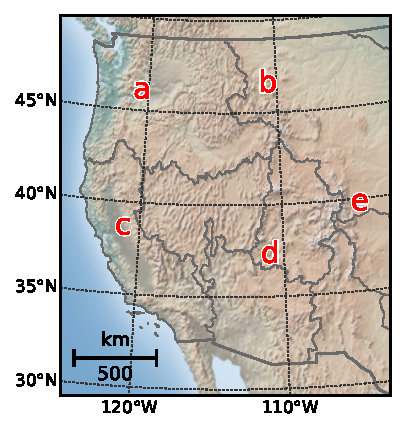
\includegraphics[width=19pc]{p2figures/fig_samplemap.pdf}}
  \caption{Western US streamflow series used in this study: (a) `Columbia River at The Dalles, OR', (b) `Missouri River at Toston, MT', (c) `Sacramento Four Index, CA' (d) `Colorado River at Lees Ferry, AZ', and (e) `South Platte River at South Platte, CO'.}\label{fig_samplemap}
\end{figure}

\begin{figure}[ht]
 \centerline{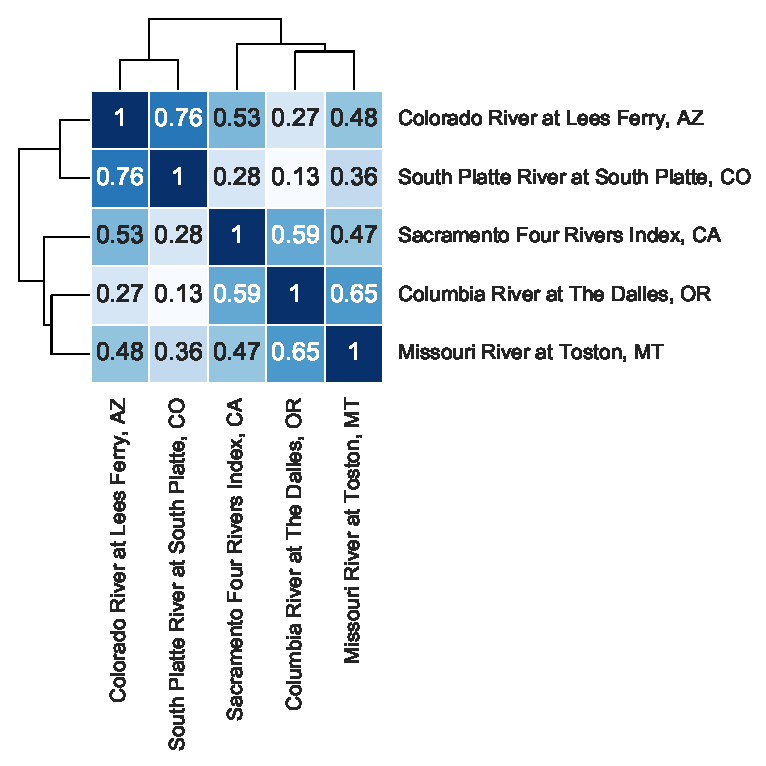
\includegraphics[width=19pc]{p2figures/fig_river_cluster.pdf}}
  \caption{Correlation matrix and clustering of interannual estimated natural streamflow series from select western US rivers basins (1930 - 2006).}\label{fig_river_cluster}
\end{figure}

\begin{figure*}[ht]
 \centerline{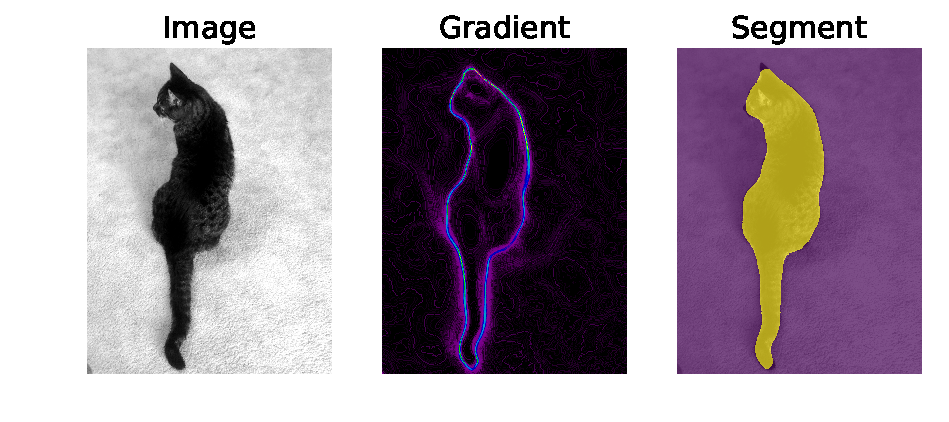
\includegraphics[width=39pc]{p2figures/fig_cat_segmentation.pdf}}
  \caption{Image segmentation used to separate the house cat from the floor in the image background. The gradient of the original image's luminance is the basis for this separation. In Figure \ref{fig_watershed_explaination}, we apply this to a geopotential height field to isolate directly ``influential'' ridge anomalies.}\label{fig_cat_segmentation}
\end{figure*}


\begin{figure}[ht]
 \centerline{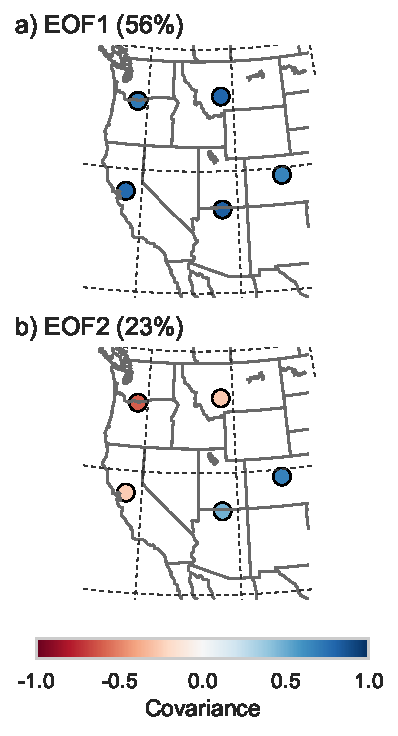
\includegraphics[width=19pc]{p2figures/fig_streamflow_eofs.pdf}}
  \caption{Leading water year streamflow PCs mapped as covariance onto the standardized natural streamflow estimate series. Figure (a) shows streamflow EOF1 - ``widespread streamflow anomalies'' - linked with DJF coastal ridge and Aleutian low variability. Figure (b) shows streamflow EOF2, or ``dipole'' variability linked to a linear hydroclimate response to ENSO teleconnections.}\label{fig_streamflow_eofs}
\end{figure}


\begin{figure}[ht]
 \centerline{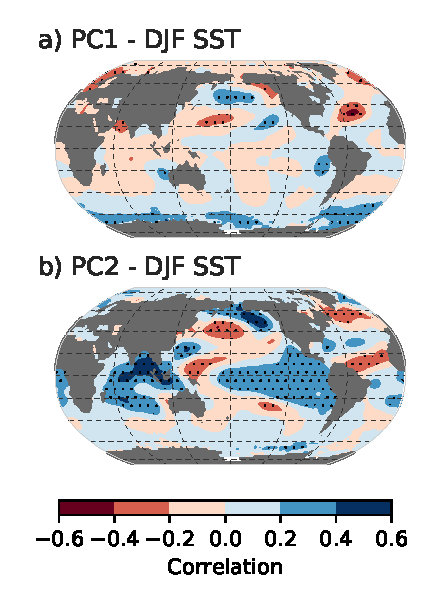
\includegraphics[width=19pc]{p2figures/fig_streamflow_pc_sst.eps}}
  \caption{Point-correlation map of streamflow PC1 (a) and PC2 (b) on DJF-mean detrended SSTs from 1930 to 2006. Note the strong equatorial Pacific correlations in (b). Shading indicated regions with local statistical significane at $\alpha = 0.05$.}\label{fig_streamflow_pc_sst}
\end{figure}

\begin{figure}[ht]
 \centerline{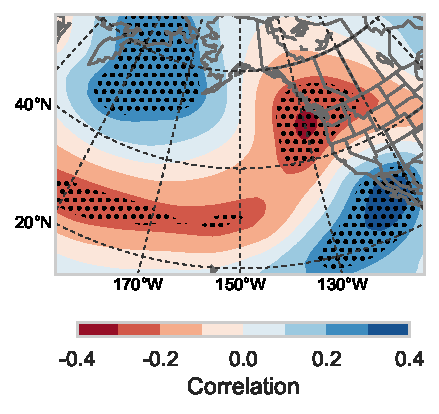
\includegraphics[width=19pc]{p2figures/fig_streamflow_pc_hgt.pdf}}
  \caption{Point-correlation map of streamflow PC1 on DJF-mean 500 mb height from 1930 to 2006. The map associates widespread dry anomalies in streamflow with ridge-like anomalies near the Pacific Northwest coast and a deepening of low anomalies near the northwest of the Aleutian Islands. Note that we did not find coastal low-anomaly near Baja California as strongly correlated or widespread in other reanalysis products within the later half of the 21st century. Shading indicates points with local statistical significane at $\alpha = 0.05$.}\label{fig_streamflow_pc_hgt}
\end{figure}

\begin{figure}[ht]
 \centerline{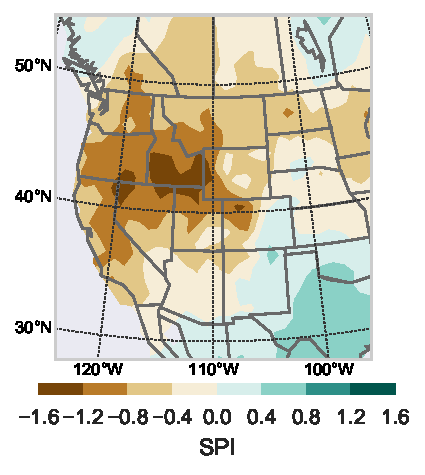
\includegraphics[width=19pc]{p2figures/fig_spi_composite.pdf}}
  \caption{Composite test showing the difference in means (positive PC years minus negative PC years) between three-month, February SPI for widespread streamflow anomalies (streamflow PC1). This shows that the widespread dry or wet streamflow anomalies in streamflow PC1 correspond with a similar variability in winter precipitation.}\label{fig_spi_composite}
\end{figure}

\begin{figure*}[ht]
 \centerline{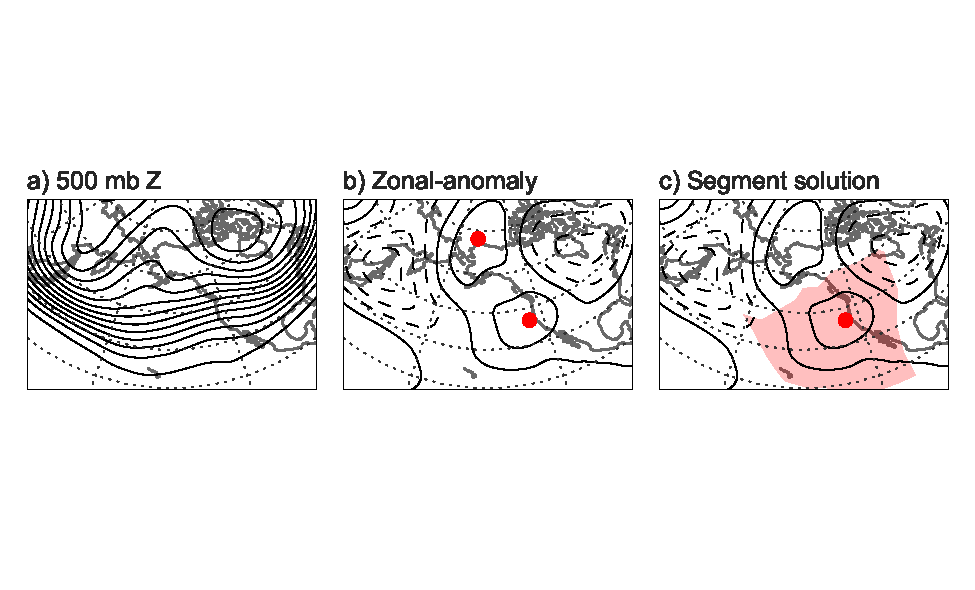
\includegraphics[width=39pc]{p2figures/fig_watershed_explanation.pdf}}
  \caption{Watershed segmentation applied to North Pacific DJF 500 mb geopotential heights for the winter of water year 1982. The original geopotential height field is shown in (a). We then use the zonal anomaly of this field to identify two ridges that are potentially influential to the West US coast. Markers (circles) are placed over these ridges (b). The north-most ridge is more intense, though the southern ridge is in closer proximity to our target region in the Pacific Northwest. The algorithm selects the southern ridge because the ridge segment (shaded area) contains our area or point of interest (c).  All contours are in intervals of 60 m.}\label{fig_watershed_explaination}
\end{figure*}

\begin{figure*}[ht]
 \centerline{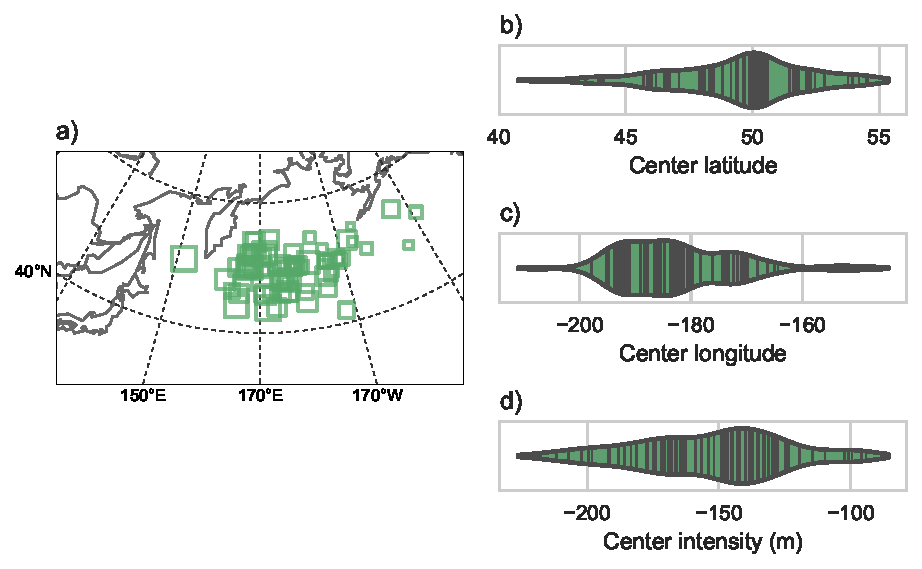
\includegraphics[width=39pc]{p2figures/fig_aleutian_stats.pdf}}
  \caption{As in Figure \ref{fig_ridge_stats} but showing DJF Aleutian low characteristics. The Aleutian low is mapped (a), with violin plots for latitude (b), longitude (c), and intensity (d). Each observation is marked with a dark line on the violin plots. Relative to the ridges we identified in Figure \ref{fig_ridge_stats}, the lows are far more confined within the North Pacific, with larger longitudinal movement and no extreme outliers to the extent that we have seen with the 1977 atmospheric ridge. The size of the mapped markers in (a) give the relative intensity of the Aleutian low.}\label{fig_aleutian_stats}
\end{figure*}

\begin{figure*}[ht]
 \centerline{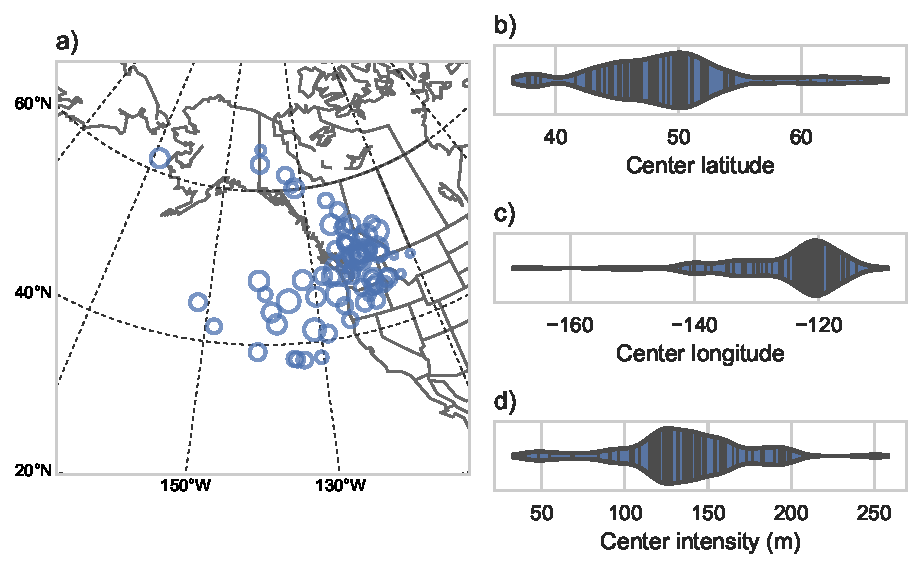
\includegraphics[width=39pc]{p2figures/fig_ridge_stats.pdf}}
  \caption{Distribution of the persistent DJF Pacific coast ridge, relating to widespread streamflow anomalies (PC1). The ridges are mapped (a), with violin plots for their latitude (b), longitude (c), and intensity (d). Each observation is marked with a dark line on the violin plots. Note the extreme outlier in ridge intensity (250.8 m) from water year 1977. The points in (a) have been slightly jittered to prevent overlapping due to the coarse resolution in the reanalysis product. The size of the mapped markers in (a) give the relative intensity of coastal ridges.}\label{fig_ridge_stats}
\end{figure*}

\begin{figure*}[ht]
 \centerline{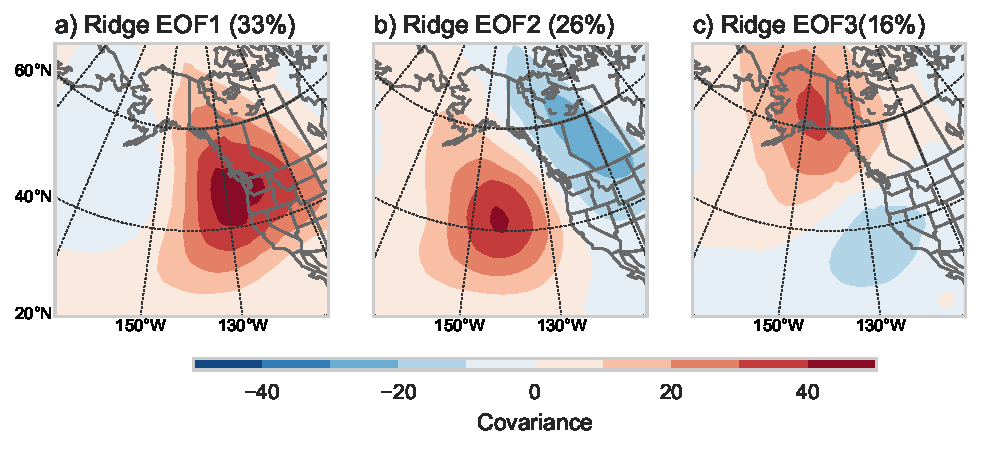
\includegraphics[width=39pc]{p2figures/fig_ridge_eofs.pdf}}
  \caption{The leading EOFs for DJF coastal ridge surfaces with time-mean removed, cut from global geopotential height fields (water year 1930 - 2006). These patterns are the leading ridge surface PCs mapped as covariance onto the geopotential height zonal-anomaly fields. The three patterns show an intensification of ridge anomalies: (a) centered over the Pacific Northwest, (b) centered off the North American Pacific coast, and (c) centered near Alaska. Similar patterns are found if this analysis is repeated in the early and later half of TCR.}\label{fig_ridge_eofs}
\end{figure*}

\begin{figure}[ht]
 \centerline{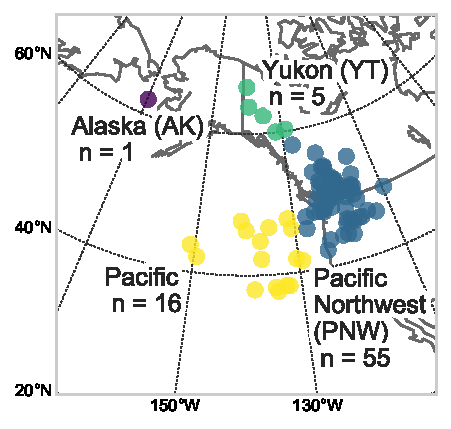
\includegraphics[width=19pc]{p2figures/fig_ridge_clustermap.pdf}}
  \caption{Clustering the 77 observed coastal ridges into five groups based on center latitude and longitude. Note the small sample size for each cluster. The distribution of streamflow for these clusters in each of the streamflow series is shown in Figure \ref{fig_streamflow_ridgecluster_violins}}\label{fig_ridge_clustermap}
\end{figure}

\begin{figure*}[ht]
 \centerline{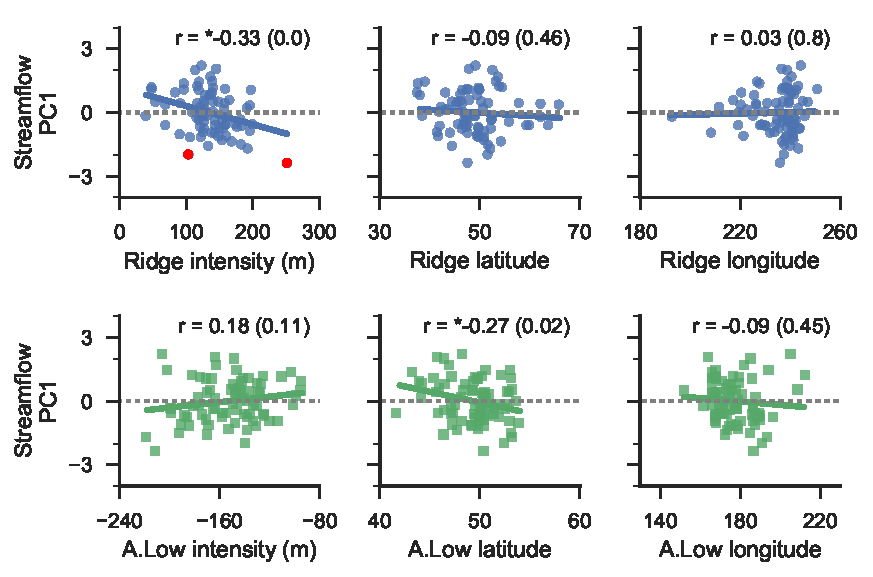
\includegraphics[width=39pc]{p2figures/fig_feature_pc1_scatter.pdf}}
  \caption{Widespread streamflow anomalies (streamflow PC1) plotted against the center intensity, latitude, and longitude for the coastal ridge (blue circles) and the Aleutian low (``A.Low'', green squares). Low values of streamflow PC1 correspond with widespread dry anomalies in west US river basins. Pearson correlation coefficient is given at the top of each plot. The parenthesis give the $p$-value for a two-sided hypothesis test. Statisticaly significant correlations are marked with ``*'' at $\alpha = 0.05$. A simple least-squares-fit line given is in each scatter plot. The highlighted points are for water year 1977 and 2002. Note the extreme intensity of the 1977 ridge. Also, note the strong dry anomaly in 2002, despite a weak-moderate ridge intensity. This is an excellent example of confounding influence from other seasons. The dry anomaly of 2002 is best explained by drought conditions later in the water year.}\label{fig_feature_pc1_scatter}
\end{figure*}

\begin{figure*}[ht]
 \centerline{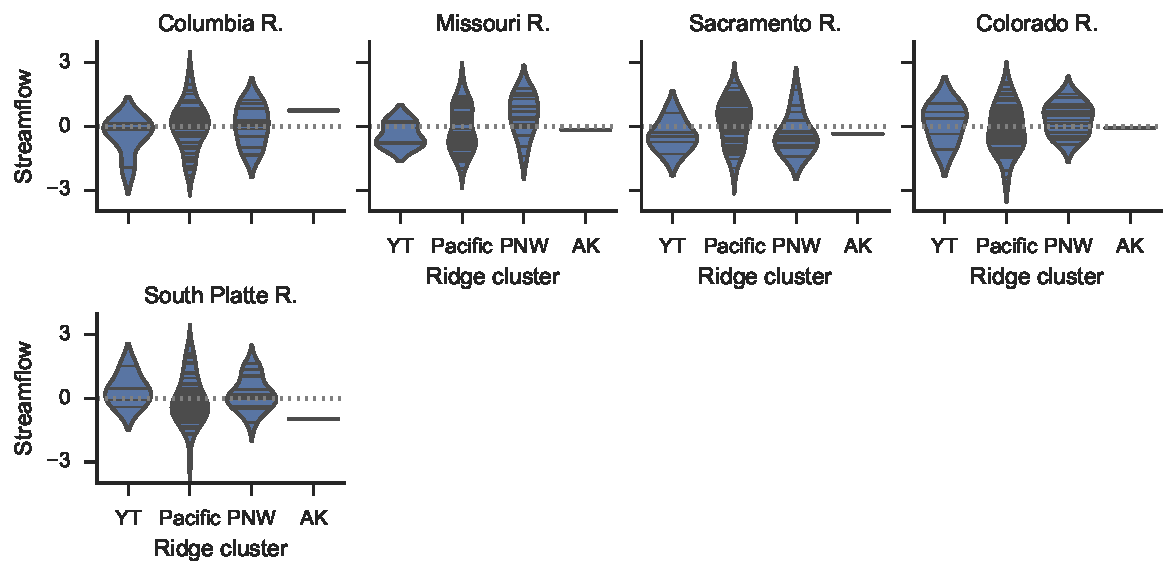
\includegraphics[width=39pc]{p2figures/fig_streamflow_ridgecluster_violins.pdf}}
  \caption{Violin plots showing the distribution of standardized streamflow series for each ridge position cluster shown in Figure \ref{fig_streamflow_ridgecluster_violins}. Ridge position clusters have a limited number of observations and streamflow distributions within these clusters are not well-defined. Individual observation are shown with a dark tick line in each violin plot. }\label{fig_streamflow_ridgecluster_violins}
\end{figure*}

\begin{figure}[ht]
 \centerline{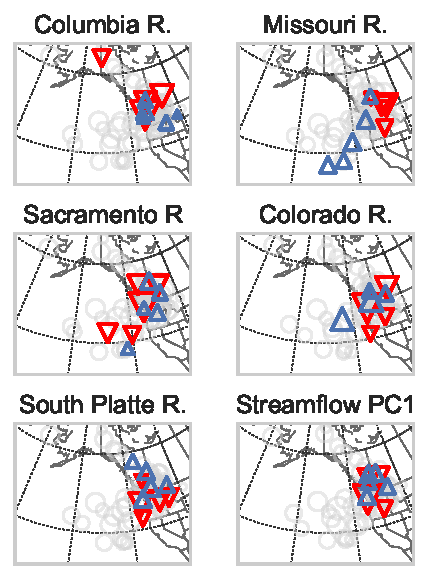
\includegraphics[width=19pc]{p2figures/fig_ridge_streamflow_position.pdf}}
  \caption{The position of the coastal ridge for the top five wet (blue, up-pointing triangle) and dry (red, down-pointing triangle) streamflow years for each river series and widespread streamflow anomalies (streamflow PC1). The size of the ridge markers give the relative intensity of ridges. }\label{fig_ridge_streamflow_position}
\end{figure}

% \bibliographystyle{ametsoc2014}
% \bibliography{references}


\begin{thebibliography}{}
\providecommand{\natexlab}[1]{#1}
\providecommand{\url}[1]{\texttt{#1}}
\renewcommand{\UrlFont}{\rmfamily}
\providecommand{\urlprefix}{URL }
\expandafter\ifx\csname urlstyle\endcsname\relax
  \providecommand{\doi}[1]{doi:\discretionary{}{}{}#1}\else
  \providecommand{\doi}{doi:\discretionary{}{}{}\begingroup
  \urlstyle{rm}\Url}\fi
\providecommand{\eprint}[2][]{\url{#2}}

\bibitem[{Beucher and Meyer(1993)Beucher, and
  Meyer}]{2dougherty_morphological_1993}
Beucher, S., and F.~Meyer, 1993: The {Morphological} {Approach} to
  {Segmentation}: {The} {Watershed} {Transformation}. \textit{Mathematical
  morphology in image processing}, E.~R. Dougherty, Ed., Optical engineering,
  M. Dekker, New York.

\bibitem[{Carrera et~al.(2004)Carrera, Higgins,, and
  Kousky}]{2carrera_downstream_2004}
Carrera, M.~L., R.~W. Higgins, and V.~E. Kousky, 2004: Downstream {Weather}
  {Impacts} {Associated} with {Atmospheric} {Blocking} over the {Northeast}
  {Pacific}. \textit{J. Climate}, \textbf{17~(24)}, 4823--4839,
  \doi{10.1175/JCLI-3237.1}.

\bibitem[{Cayan and Peterson(1989)Cayan, and Peterson}]{2cayan_influence_1989}
Cayan, D.~R., and D.~H. Peterson, 1989: The {Influence} of {North} {Pacific}
  {Atmospheric} {Circulation} on {Streamflow} in the {West}. \textit{Aspects of
  {Climate} {Variability} in the {Pacific} and the {Western} {Americas}}, D.~H.
  Peterson, Ed., American Geophysical Union, Washington, D. C., 375--397,
  doi: 10.1029/GM055p0375.

\bibitem[{Cayan et~al.(1999)Cayan, Redmond,, and Riddle}]{2cayan_enso_1999}
Cayan, D.~R., K.~T. Redmond, and L.~G. Riddle, 1999: {ENSO} and {Hydrologic}
  {Extremes} in the {Western} {United} {States}. \textit{J. Clim.},
  \textbf{12~(9)}, 2881--2893,
  \doi{10.1175/1520-0442(1999)012<2881:EAHEIT>2.0.CO;2}.

\bibitem[{Chang et~al.(2015)Chang, Zheng, Lanigan, Yau,, and
  Neelin}]{2chang_significant_2015}
Chang, E. K.~M., C.~Zheng, P.~Lanigan, A.~M.~W. Yau, and J.~D. Neelin, 2015:
  Significant modulation of variability and projected change in {California}
  winter precipitation by extratropical cyclone activity. \textit{Geophys. Res.
  Lett.}, \textbf{42~(14)}, 2015GL064\,424, \doi{10.1002/2015GL064424}.

\bibitem[{\textit{Changnon et~al.}(1991)\textit{Changnon, McKee, and
  Doesken}}]{2changnon_hydroclimatic_1991}
Changnon, D., T.~B. McKee, and N.~J. Doesken (1991), Hydroclimatic variability
  in the {Rocky} {Mountains}, \textit{J Am Water Resources Assoc},
  \textit{27}(5), 733--743, \doi{10.1111/j.1752-1688.1991.tb01471.x}.

\bibitem[{Choi et~al.(2016)Choi, Lu, Son, Frierson,, and
  Yoon}]{2choi_uncertainty_2016}
Choi, J., J.~Lu, S.-W. Son, D.~M.~W. Frierson, and J.-H. Yoon, 2016:
  Uncertainty in future projections of the {North} {Pacific} subtropical high
  and its implication for {California} winter precipitation change. \textit{J.
  Geophys. Res. Atmos.}, \textbf{121~(2)}, 2015JD023\,858,
  \doi{10.1002/2015JD023858}.

\bibitem[{Compo et~al.(2011)}]{2compo_twentieth_2011}
Compo, G.~P., and Coauthors, 2011: The {Twentieth} {Century} {Reanalysis}
  {Project}. \textit{Quarterly Journal of the Royal Meteorological Society},
  \textbf{137~(654)}, 1--28, \doi{10.1002/qj.776}.

\bibitem[{Cook et~al.(2014)Cook, Seager,, and Smerdon}]{2cook_worst_2014}
Cook, B.~I., R.~Seager, and J.~E. Smerdon, 2014: The worst {North} {American}
  drought year of the last millennium: 1934. \textit{Geophys. Res. Lett.},
  \textbf{41~(20)}, 7298--7305, \doi{10.1002/2014GL061661}.

\bibitem[{Cousty et~al.(2009)Cousty, Bertrand, Najman,, and
  Couprie}]{2cousty_watershed_2009}
Cousty, J., G.~Bertrand, L.~Najman, and M.~Couprie, 2009: Watershed {Cuts}:
  {Minimum} {Spanning} {Forests} and the {Drop} of {Water} {Principle}.
  \textit{IEEE Transactions on Pattern Analysis and Machine Intelligence},
  \textbf{31~(8)}, 1362--1374, \doi{10.1109/TPAMI.2008.173}.

\bibitem[{Dawson(2016)}]{2dawson_eofs:_2016}
Dawson, A., 2016: eofs: {A} {Library} for {EOF} {Analysis} of {Meteorological},
  {Oceanographic}, and {Climate} {Data}. \textit{Journal of Open Research
  Software}, \textbf{4~(1)}, \doi{10.5334/jors.122}.

\bibitem[{Dettinger et~al.(2015)Dettinger, Udall,, and
  Georgakakos}]{2dettinger_western_2015}
Dettinger, M., B.~Udall, and A.~Georgakakos, 2015: Western water and climate
  change. \textit{Ecological Applications}, \textbf{25~(8)}, 2069--2093,
  \doi{10.1890/15-0938.1}.

\bibitem[{Digabel and Lantuejoul(1978)Digabel, and
  Lantuejoul}]{2digabel_iterative_1978}
Digabel, H., and C.~Lantuejoul, 1978: Iterative {Algorithms}.
  \textit{Proceedings of the 2nd European Symposium Quantitative Analysis of
  Microstructures in Material Science, Biology and Medicine}, 85--89.

\bibitem[{Frierson et~al.(2007)Frierson, Lu,, and Chen}]{2frierson_width_2007}
Frierson, D. M.~W., J.~Lu, and G.~Chen, 2007: Width of the {Hadley} cell in
  simple and comprehensive general circulation models. \textit{Geophys. Res.
  Lett.}, \textbf{34~(18)}, L18\,804, \doi{10.1029/2007GL031115}.

\bibitem[{Hamlet et~al.(2005)Hamlet, Mote, Clark,, and
  Lettenmaier}]{2hamlet_effects_2005}
Hamlet, A.~F., P.~W. Mote, M.~P. Clark, and D.~P. Lettenmaier, 2005: Effects of
  {Temperature} and {Precipitation} {Variability} on {Snowpack} {Trends} in the
  {Western} {United} {States}. \textit{Journal of Climate}, \textbf{18~(21)},
  4545--4561.

\bibitem[{Hamlet et~al.(2007)Hamlet, Mote, Clark,, and
  Lettenmaier}]{2hamlet_twentieth-century_2007}
Hamlet, A.~F., P.~W. Mote, M.~P. Clark, and D.~P. Lettenmaier, 2007:
  Twentieth-{Century} {Trends} in {Runoff}, {Evapotranspiration}, and {Soil}
  {Moisture} in the {Western} {United} {States}. \textit{J. Climate},
  \textbf{20~(8)}, 1468--1486, \doi{10.1175/JCLI4051.1}.

\bibitem[{Hodges(1994)}]{2hodges_general_1994}
Hodges, K.~I., 1994: A {General} {Method} for {Tracking} {Analysis} and {Its}
  {Application} to {Meteorological} {Data}. \textit{Monthly Weather Review},
  \textbf{122~(11)}, 2573--2586,
  \doi{10.1175/1520-0493(1994)122<2573:AGMFTA>2.0.CO;2}.

\bibitem[{Hoskins and Hodges(2002)Hoskins, and Hodges}]{2hoskins_new_2002}
Hoskins, B.~J., and K.~I. Hodges, 2002: New {Perspectives} on the {Northern}
  {Hemisphere} {Winter} {Storm} {Tracks}. \textit{Journal of the Atmospheric
  Sciences}, \textbf{59~(6)}, 1041--1061,
  \doi{10.1175/1520-0469(2002)059<1041:NPOTNH>2.0.CO;2}.

\bibitem[{Huang et~al.(2014)}]{2huang_extended_2014}
Huang, B., and Coauthors, 2014: Extended {Reconstructed} {Sea} {Surface}
  {Temperature} {Version} 4 ({ERSST}.v4). {Part} {I}: {Upgrades} and
  {Intercomparisons}. \textit{Journal of Climate}, \textbf{28~(3)}, 911--930,
  \doi{10.1175/JCLI-D-14-00006.1}.

\bibitem[{Huang et~al.(2015)}]{2huang_further_2015}
Huang, B., and Coauthors, 2015: Further {Exploring} and {Quantifying}
  {Uncertainties} for {Extended} {Reconstructed} {Sea} {Surface} {Temperature}
  ({ERSST}) {Version} 4 (v4). \textit{Journal of Climate}, \textbf{29~(9)},
  3119--3142, \doi{10.1175/JCLI-D-15-0430.1}.
  
\bibitem[{Kalnay et~al.(1996)}]{2kalnay_ncep/ncar_1996}
Kalnay, E., and Coauthors, 1996: The {NCEP}/{NCAR} 40-{Year} {Reanalysis}
  {Project}. \textit{Bull. Amer. Meteor. Soc.}, \textbf{77~(3)}, 437--471,
  \doi{10.1175/1520-0477(1996)077<0437:TNYRP>2.0.CO;2}.

\bibitem[{Lambert(1988)}]{2lambert_cyclone_1988}
Lambert, S.~J., 1988: A {Cyclone} {Climatology} of the {Canadian} {Climate}
  {Centre} {General} {Circulation} {Model}. \textit{Journal of Climate},
  \textbf{1~(1)}, 109--115,
  \doi{10.1175/1520-0442(1988)001<0109:ACCOTC>2.0.CO;2}.

\bibitem[{Langenbrunner et~al.(2015)Langenbrunner, Neelin, Lintner,, and
  Anderson}]{2langenbrunner_patterns_2015}
Langenbrunner, B., J.~D. Neelin, B.~R. Lintner, and B.~T. Anderson, 2015:
  Patterns of {Precipitation} {Change} and {Climatological} {Uncertainty} among
  {CMIP}5 {Models}, with a {Focus} on the {Midlatitude} {Pacific} {Storm}
  {Track}. \textit{J. Climate}, \textbf{28~(19)}, 7857--7872,
  \doi{10.1175/JCLI-D-14-00800.1}.

\bibitem[{Lins(1997)}]{2lins_regional_1997}
Lins, H.~F., 1997: Regional streamflow regimes and hydroclimatology of the
  {United} {States}. \textit{Water Resour. Res.}, \textbf{33~(7)}, 1655--1667,
  \doi{10.1029/97WR00615}.

\bibitem[{Liu et~al.(2014)}]{2liu_extended_2014}
Liu, W., and Coauthors, 2014: Extended {Reconstructed} {Sea} {Surface}
  {Temperature} {Version} 4 ({ERSST}.v4): {Part} {II}. {Parametric} and
  {Structural} {Uncertainty} {Estimations}. \textit{Journal of Climate},
  \textbf{28~(3)}, 931--951, \doi{10.1175/JCLI-D-14-00007.1}.

\bibitem[{Malevich and Woodhouse(2016)Malevich, and
  Woodhouse}]{2malevich_pacific_2016}
Malevich, S.~B., and C.~A. Woodhouse, 2016: Pacific {SSTs}, mid-latitude
  atmospheric circulation, and widespread interannual anomalies in {Western}
  {US} streamflow. In prep. \textit{Geophys. Res. Lett.}

\bibitem[{McKee et~al.(1993)McKee, Doesken,, and
  Kleist}]{2mckee_relationship_1993}
McKee, T.~B., N.~J. Doesken, and J.~Kleist, 1993: The relationship of drought
  frequency and druration to time scales. \textit{Proceedings of the 8th
  {Conference} on {Applied} {Climatology}}, American Meteorolical Society,
  Boston, MA, 22, Vol.~17, 179--183.

\bibitem[{Murray and Simmonds(1991)Murray, and
  Simmonds}]{2murray_numerical_1991}
Murray, R., and I.~Simmonds, 1991: A numerical scheme for tracking cyclone
  centres from digital data. {Part} {I}: {Development} and operation of the
  scheme. \textit{Austrailian Meteorological Magazine}, \textbf{39}, 155--166.

\bibitem[{National Center~for Atmospheric~Research(2013)}]{2cisl_rda_ds2980}
National Center~for Atmospheric~Research, U. C. f. A.~R., 2013: Standardized
  precipitation index (spi) for global land surface (1949-2012). Research Data
  Archive at the National Center for Atmospheric Research, Computational and
  Information Systems Laboratory, Boulder CO,
  \urlprefix\url{https://doi.org/10.5065/D6086397}.

\bibitem[{Neelin et~al.(2013)Neelin, Langenbrunner, Meyerson, Hall,, and
  Berg}]{2neelin_california_2013}
Neelin, J.~D., B.~Langenbrunner, J.~E. Meyerson, A.~Hall, and N.~Berg, 2013:
  California {Winter} {Precipitation} {Change} under {Global} {Warming} in the
  {Coupled} {Model} {Intercomparison} {Project} {Phase} 5 {Ensemble}.
  \textit{J. Climate}, \textbf{26~(17)}, 6238--6256,
  \doi{10.1175/JCLI-D-12-00514.1}.

\bibitem[{North et~al.(1982)North, Bell, Cahalan,, and
  Moeng}]{2north_sampling_1982}
North, G.~R., T.~L. Bell, R.~F. Cahalan, and F.~J. Moeng, 1982: Sampling
  {Errors} in the {Estimation} of {Empirical} {Orthogonal} {Functions}.
  \textit{Mon. Wea. Rev.}, \textbf{110~(7)}, 699--706,
  \doi{10.1175/1520-0493(1982)110<0699:SEITEO>2.0.CO;2}.

\bibitem[{Overland et~al.(1999)Overland, Adams,, and
  Bond}]{2overland_decadal_1999}
Overland, J.~E., J.~M. Adams, and N.~A. Bond, 1999: Decadal {Variability} of
  the {Aleutian} {Low} and {Its} {Relation} to {High}-{Latitude} {Circulation}.
  \textit{J. Climate}, \textbf{12~(5)}, 1542--1548,
  \doi{10.1175/1520-0442(1999)012<1542:DVOTAL>2.0.CO;2}.

\bibitem[{O’Loughlin et~al.(2012)O’Loughlin, Witmer, Linke, Laing,
  Gettelman,, and Dudhia}]{2oloughlin_climate_2012}
O’Loughlin, J., F.~D.~W. Witmer, A.~M. Linke, A.~Laing, A.~Gettelman, and
  J.~Dudhia, 2012: Climate variability and conflict risk in {East} {Africa},
  1990–2009. \textit{Proceedings of the National Academy of Sciences},
  \textbf{109~(45)}, 18\,344--18\,349, \doi{10.1073/pnas.1205130109}.

\bibitem[{Redmond and Koch(1991)Redmond, and Koch}]{2redmond_surface_1991}
Redmond, K.~T., and R.~W. Koch, 1991: Surface {Climate} and {Streamflow}
  {Variability} in the {Western} {United} {States} and {Their} {Relationship}
  to {Large}-{Scale} {Circulation} {Indices}. \textit{Water Resour. Res.},
  \textbf{27~(9)}, 2381--2399, \doi{10.1029/91WR00690}.

\bibitem[{Scheff and Frierson(2012)Scheff, and
  Frierson}]{2scheff_twenty-first-century_2012}
Scheff, J., and D.~Frierson, 2012: Twenty-{First}-{Century} {Multimodel}
  {Subtropical} {Precipitation} {Declines} {Are} {Mostly} {Midlatitude}
  {Shifts}. \textit{J. Climate}, \textbf{25~(12)}, 4330--4347,
  \doi{10.1175/JCLI-D-11-00393.1}.

\bibitem[{Seager et~al.(2014)Seager, Hoerling, Schubert, Wang, Lyon, Kumar,
  Nakamura,, and Henderson}]{2seager_causes_2014}
Seager, R., M.~Hoerling, S.~Schubert, H.~Wang, B.~Lyon, A.~Kumar, J.~Nakamura,
  and N.~Henderson, 2014: Causes and {Predictability} of the 2011 to 2014
  {California} {Drought}. Tech. rep., National Oceanic and Atmospheric
  Administration, Washington, D.C.

\bibitem[{Seager et~al.(2015)Seager, Hoerling, Schubert, Wang, Lyon, Kumar,
  Nakamura,, and Henderson}]{2seager_causes_2015}
Seager, R., M.~Hoerling, S.~Schubert, H.~Wang, B.~Lyon, A.~Kumar, J.~Nakamura,
  and N.~Henderson, 2015: Causes of the 2011–14 {California} {Drought}.
  \textit{J. Climate}, \textbf{28~(18)}, 6997--7024,
  \doi{10.1175/JCLI-D-14-00860.1}.

\bibitem[{Sheppard et~al.(2002)Sheppard, Comrie, Packin, Angersbach,, and
  Hughes}]{2sheppard_climate_2002}
Sheppard, P.~R., A.~C. Comrie, G.~D. Packin, K.~Angersbach, and M.~K. Hughes,
  2002: The climate of the {US} {Southwest}. \textit{Climate Research},
  \textbf{21}, 219--238.

\bibitem[{Swain(2015)}]{2swain_tale_2015}
Swain, D.~L., 2015: A tale of two {California} droughts: {Lessons} amidst
  record warmth and dryness in a region of complex physical and human
  geography. \textit{Geophys. Res. Lett.}, 2015GL066628,
  \doi{10.1002/2015GL066628}.

\bibitem[{Vincent and Soille(1991)Vincent, and
  Soille}]{2vincent_watersheds_1991}
Vincent, L., and P.~Soille, 1991: Watersheds in digital spaces: an efficient
  algorithm based on immersion simulations. \textit{IEEE Transactions on
  Pattern Analysis and Machine Intelligence}, \textbf{13~(6)}, 583--598,
  \doi{10.1109/34.87344}.

\bibitem[{Wallace and Gutzler(1981)Wallace, and
  Gutzler}]{2wallace_teleconnections_1981}
Wallace, J.~M., and D.~S. Gutzler, 1981: Teleconnections in the {Geopotential}
  {Height} {Field} during the {Northern} {Hemisphere} {Winter}. \textit{Monthly
  Weather Review}, \textbf{109~(4)}, 784--812.

\bibitem[{Wilks(2006)}]{2wilks_statistical_2006}
Wilks, D., 2006: \textit{Statistical {Methods} in the {Atmospheric}
  {Sciences}}. 2nd ed., International geophysics series, Academic Press,
  London, UK.

\bibitem[{Wise(2016)}]{2wise_five_2016}
Wise, E.~K., 2016: Five centuries of {U}.{S}. {West} {Coast} drought:
  {Occurrence}, spatial distribution, and associated atmospheric circulation
  patterns. \textit{Geophys. Res. Lett.}, \textbf{43~(9)}, 2016GL068\,487,
  \doi{10.1002/2016GL068487}.

\bibitem[{Wise and Dannenberg(2014)Wise, and
  Dannenberg}]{2wise_persistence_2014}
Wise, E.~K., and M.~P. Dannenberg, 2014: Persistence of pressure patterns over
  {North} {America} and the {North} {Pacific} since {AD} 1500. \textit{Nat
  Commun}, \textbf{5}, \doi{10.1038/ncomms5912}.

\end{thebibliography}

\chapter{Supplemental Information for The importance of coastal Pacific ridge and Aleutian low position and intensity for widespread interannual anomalies in western US streamflow}

\section{Segmentation example}

A very simple example of coding a segmentation problem on the December, 1981 monthly mean 500 mb geopotential height from 20CR. Type in \verb|this font| is code intended to be run in an interactive Python session.

We begin by importing needed modules into our session.

\begin{singlespacing}
\begin{verbatim}
import numpy as np
import pandas as pd
import xarray as xr
import matplotlib.pylab as plt
import cartopy.crs as ccrs
from scipy import ndimage
from skimage.feature import peak_local_max
from skimage.morphology import watershed
\end{verbatim}
\end{singlespacing}

 Now set some global variables. You should change these to examine a different time, or reanalysis product path.

\begin{singlespacing}
\begin{verbatim}
TARGET_TIME = '1981-12-01'
NC_PATH = 'hgt.mon.mean.nc'  # 20CR monthly mean geo hgt
\end{verbatim}
\end{singlespacing}

Now we read in the netCDF file, copying our target time-slice and level into memory, and then closing the file.

\begin{singlespacing}
\begin{verbatim}
with xr.open_dataset(NC_PATH) as d:
    hgt = (d.hgt.sel(level = 500, time = TARGET_TIME)
                .copy())
\end{verbatim}
\end{singlespacing}

Here is a simple map of the monthly average field we just imported (Figure \ref{fig_example_out1}).

\begin{singlespacing}
\begin{verbatim}
ax = plt.axes(projection = ccrs.Orthographic(-140, 42))
ax.set_global()
hgt.plot.contourf(ax = ax, transform = ccrs.PlateCarree())
ax.coastlines()
ax.gridlines()
\end{verbatim}
\end{singlespacing}

\begin{figure}[h]
 \centerline{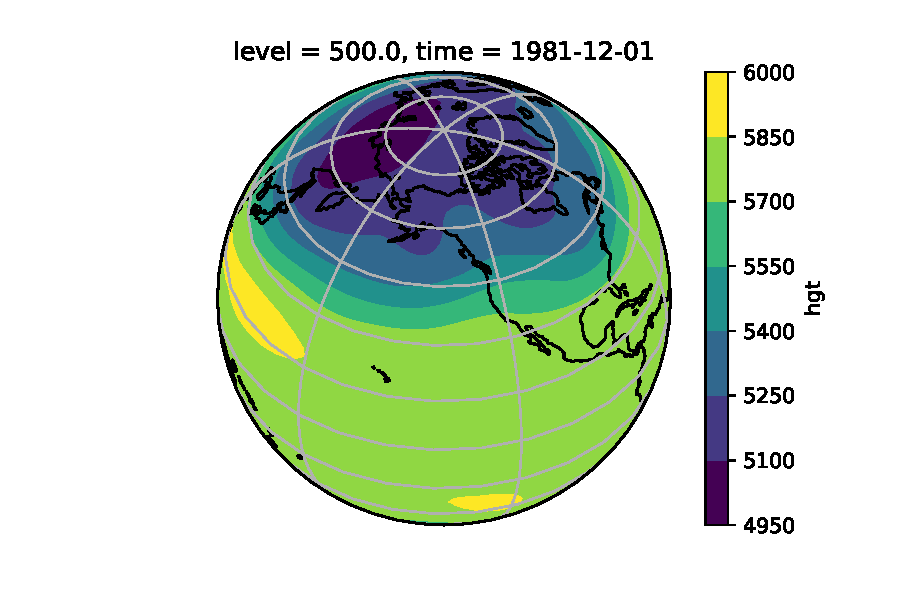
\includegraphics[width=19pc]{p2figures/fig_example_out1.pdf}}
  \caption{A vanilla 500 mb geopotential height field projected onto an orthographic map.}\label{fig_example_out1}
\end{figure}

Now we remove the zonal-mean from the field, creating the zonal-anomaly (Figure \ref{fig_example_out3}).

\begin{singlespacing}
\begin{verbatim}
zonal_mean = hgt.mean(dim = 'lon')
eddy = hgt - zonal_mean

ax = plt.axes(projection = ccrs.PlateCarree(-180))
ax.set_global()
eddy.plot(ax = ax, transform = ccrs.PlateCarree())
ax.coastlines()
ax.gridlines()
\end{verbatim}
\end{singlespacing}

\begin{figure}[h]
 \centerline{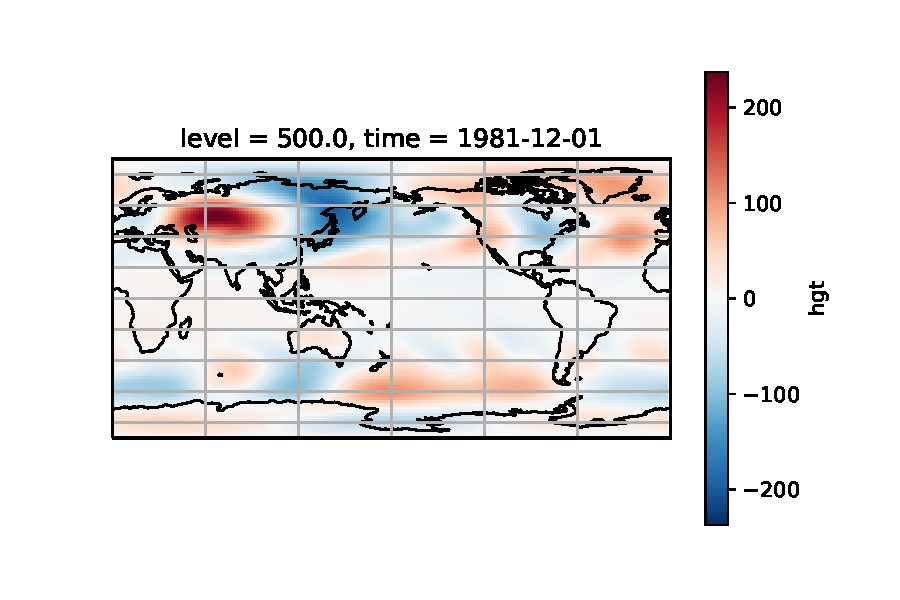
\includegraphics[width=19pc]{p2figures/fig_example_out3.pdf}}
  \caption{Zonal-anomaly of the 500 mb height field with coastlines.}\label{fig_example_out3}
\end{figure}

We then find local maxima, our ``markers'', on the zonal-anomaly field (Figure \ref{fig_example_out4}.

\begin{singlespacing}
\begin{verbatim}
local_maxi = peak_local_max(eddy.values,
                            exclude_border = False,
                            indices = False,
                            min_distance = 3)

markers, n_marks = ndimage.label(local_maxi,
                                 structure = np.ones((3, 3)))
plt.pcolor(markers)
\end{verbatim}
\end{singlespacing}

\begin{figure}[h]
 \centerline{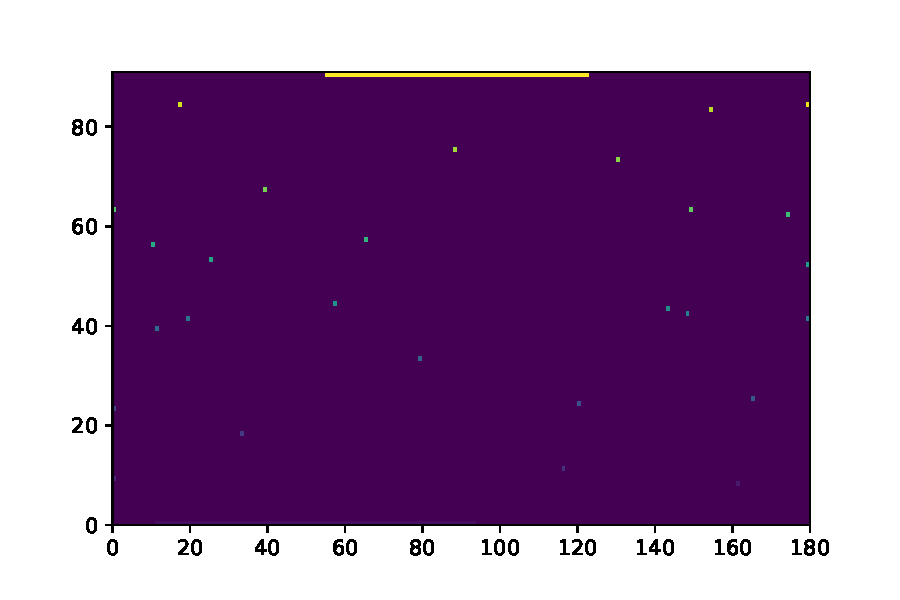
\includegraphics[width=19pc]{p2figures/fig_example_out4.pdf}}
  \caption{The position of pixel markers on the 500 mb zonal-anomaly field.}\label{fig_example_out4}
\end{figure}

Now, we use the markers and the original zonal-anomaly surface for segmentation (shown in Figure \ref{fig_example_out5}). Note that we need to flip the zonal-anomaly field.

\begin{singlespacing}
\begin{verbatim}
segments = watershed(-1 * eddy.values, markers)
plt.pcolor(segments)
\end{verbatim}
\end{singlespacing}

\begin{figure}[h]
 \centerline{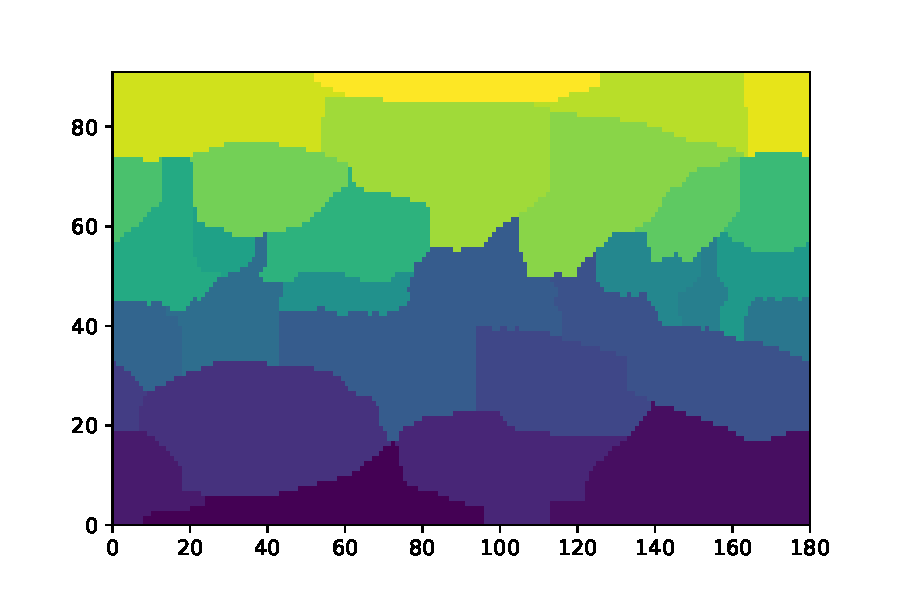
\includegraphics[width=19pc]{p2figures/fig_example_out5.pdf}}
  \caption{Waterhsed segments found from the markers placed on the zonal-anomaly field.}\label{fig_example_out5}
\end{figure}

We can quickly create a crude plot that shows these segments on a global map (Figure \ref{fig_example_out6}).

\begin{singlespacing}
\begin{verbatim}
eddy['segments'] = (('lat', 'lon'), segments)
ax = plt.axes(projection = ccrs.PlateCarree(-180))
ax.contour(eddy.lon, eddy.lat, eddy, colors = 'k', 
           linewidth = 0.5,
           levels = np.arange(-480, 480, 60), 
           transform = ccrs.PlateCarree())
eddy['segments'].plot(ax = ax, 
                      transform = ccrs.PlateCarree(),
                      add_colorbar = False, cmap = 'Set2')
ax.coastlines()
ax.gridlines()
\end{verbatim}
\end{singlespacing}

\begin{figure}[h]
 \centerline{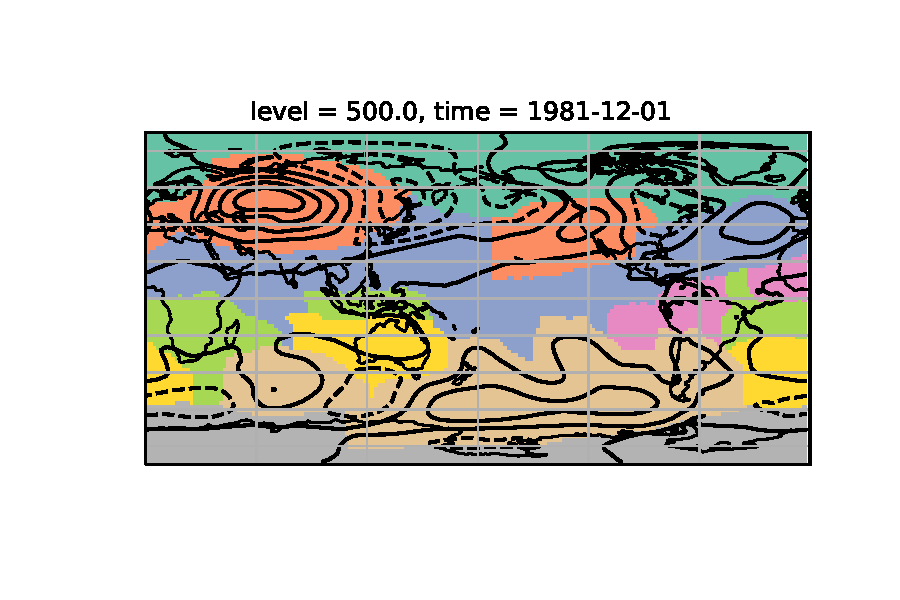
\includegraphics[width=19pc]{p2figures/fig_example_out6.pdf}}
  \caption{Watershed segments, recolored and projected onto a map with contours giving the original zonal-anomaly.}\label{fig_example_out6}
\end{figure}

As you can see from Figure \ref{fig_example_out6}, the results are reasonable over the midlatitudes but care is needed when approaching the tropics or worse, the edges of a climate field. Here, it becomes important to regrid the data, code your algorithm to properly wrap-around, or use flipped or mirrored extensions on the field edges.

\chapter{Extreme widespread Western US precipitation anomalies and wintertime Pacific coast atmospheric ridges in the CESM Large Ensemble historical simulations}

\section{Abstract}
Internal climate variability and spatially widespread precipitation anomalies can have a dramatic impact on water supplies in the western United States. In this study we examine the 35 historical (1920 - 2005) runs of the CESM Large Ensemble to determine whether this ensemble - which attempts to explicitly quantify internal variability -  is able to simulate extremely widespread, dry winter precipitation anomalies that are comparable to the extreme 1976 - 1977 drought event. We find 36 events across the 35 ensemble members. We show that these events have a strong and significant association with anomalously intense atmospheric ridges near the coastal Pacific Northwest. The spatial pattern of these simulated extreme events is relatively similar to the observed 1976 - 1977 event.

\section{Introduction}


Among the most concerning aspects of climate change is the potential impact to water supplies. Globally, the differences between wet and dry regions and seasons are likely to increase under a warmer climate due to a ``rich-get-richer'' mechanism \citep{3ipcc_climate_2013}. This mechanism can be loosely summarized with the Clausius-Clapeyron relation, connecting increased air temperature with increased atmospheric water vapor, thus with global warming we may generally see increased precipitation in the midlatitudes and tropics, but decreased precipitation in the subtropics \citep{3manabe_effects_1975, 3held_robust_2006}. An additional impact on regional water supplies may come from projected shifts in atmospheric circulation \citep{3lu_expansion_2007, 3scheff_twenty-first-century_2012}. But there is considerable uncertainty in these projections for some regions, like the eastern North Pacific. This uncertainty in multimodel studies appears to stem from differences in simulated Pacific ocean-atmosphere interactions, and more generally, the diverse structure of the global climate models used in these projections \citep[e.g., ][]{3langenbrunner_patterns_2015, 3choi_uncertainty_2016, 3reclamation_bureau_of_reclamation_west-wide_2016}. However, another key source of uncertainty is internal climate variability, which is especially important for the eastern North Pacific and a concern for water supplies in the western United States (US) \citep{3reclamation_bureau_of_reclamation_west-wide_2016}.

In the western US, climate change threatens to compound the problems of water management by stressing water resources that are already pushed to, or beyond, their natural limits \citep{3dettinger_western_2015}. Water resource management challenges will be complicated not just by especially long-lasting droughts, but by droughts with spatially widespread impact. Some of the most extreme and widespread impacts are associated with seasonal changes in the position and intensity of the semi-permanent atmospheric ridge off the Pacific Northwest coast of North America. Nicknamed the ``ridiculously resilient ridge'' for its role in the 2010s California drought. Such a feature was also a direct driver of the extreme 1977 drought in the West. Ridges in this region can disrupt and divert cool-season moisture-delivery into the western US, affecting not just precipitation but high-elevation snowpack and annual streamflow anomalies throughout the region. Several recent studies have documented the significant multimodel uncertainty in the eastern North Pacific atmospheric circulation and its impact on precipitation projections within the western US \citep[e.g., ][]{3langenbrunner_patterns_2015, 3choi_uncertainty_2016}. Few studies have explored how these extreme, widespread dry events relating to anomalously intense coastal ridges are represented in large-ensemble climate model products that are designed to explicitly estimate for internal climate variability \citep[e.g., ][]{3kay_community_2014}.

In order to assess the ability of climate models to replicate relationships between coastal ridges and widespread precipitation anomalies in the western US, we apply an object-tracking framework - similar to that used to create stormtrack/cyclone records, using a segmentation algorithm to locate the position and intensity of influential coastal atmospheric ridges along the Pacific Northwest coast of North America in the Community Earth System Model Large Ensemble (CESMLE) \citep{3kay_community_2014}. We locate wintertime ridges in the 35 members of the CESMLE, using runs from 1920 - 2005 with each ensemble member utilizing the same model under identical forcing. This is used as a simulated estimate of the ``internal variability'' of the coastal ridge under historical climate conditions. We examine the association between simulated coastal ridge variability and extreme, spatially widespread precipitation anomalies within the western US in order to estimate how well the CESMLE represents extreme 1977-like droughts.

Specifically, this paper addresses the following question: How well does the CESMLE represent the wintertime coastal ridge's potentially widespread impact on precipitation under the observed climate variability of the past nine decades. We first describe the data we used for this study and explain our use of segmentation algorithms to identify coastal ridges. We then define mean bias in the simulations by comparing CESMLE historical climatology with that from reanalysis products. Finally, we examine the frequency of 1977-like droughts in the CESMLE and how strongly and consistently these events relate to winters with anomalously strong, coastal atmospheric ridges in the Pacific Northwest.

\section{Data}


Simulated precipitation and 500 mb geopotential height fields were obtained from the 35 model CESMLE members \citep{3kay_community_2014}. These members all use the same model, the Community Earth System Model v1 and the Community Atmosphere Model v5.5 \citep{3hurrell_community_2013}. The model components are all run with 1\textdegree~ horizontal resolution. Each of these member runs extend from 1920 - 2005, with the exception of the first ensemble member which begins in 1850, and was cropped to 1920 - 2005 in order to match the other ensemble runs. CESMLE members all use the same historical forcing up to 2005 and then continue under Representative Concentration Pathway 8.5 (RCP85) from 2005 to 2100 \citep{3kay_community_2014}. Each ensemble member was started with slightly different initializing conditions, to explicitly estimate the simulation's internal climate variability. See \citet{3kay_community_2014} for a discussion of CESMLE simulations relative to the Coupled Model Intercomparison Project Phase 5 (CMIP5) ensemble.

We compared the historical CESMLE runs with different ``observed'' climate field products. For precipitation, we used the Global Precipitation Climatology Center version 7 (GPCC) full data, monthly product, cropped to 1920 - 2005 to match the CESMLE historical simulations \citep{3schneider_gpcc_2015}. We used the 0.5\textdegree~ resolution fields. For 500 mb geopotential height, we used the ensemble-mean NOAA-CIRES Twentieth Century Reanalysis version 2c (20CR), which have a spatial resolution of 2\textdegree~ \citep{3compo_twentieth_2011}. Daily 20CR fields were cropped to 1920 - 2005 to match the CESMLE historical simulations. We also checked CESMLE climatology for bias against the daily ERA-Interim reanalysis (ERA-I) \citep{3dee_era-interim_2011} and Global Precipitation Climatology Project (GPCP) v2.3 fields \citep{3adler_version-2_2003} from 1980 - 2005. GPCP has a 2.5\textdegree~ spatial resolution. ERA-I has an approximate 80 km spatial resolution. 

We regridded all products into an approximate 1\textdegree~ by 1\textdegree~ grid, matching the CESMLE. All fields were averaged into winter (DJF) fields. We focus on this season because it is associated with well-organized atmospheric circulation and cohesive semi-permanent air masses.

Our ridge-identification method used zonal-anomaly geopotential height fields. These were created by removing the longitudinal average from each time observation in a geopotential height field. This makes ridge and trough anomalies easily identifiable on the geopotential height surfaces.

\section{Methods}


\subsection{Climatology \& ensemble mean bias}

We defined climatology using the mean of each gridded observational product and the CESMLE mean from 1920 - 2005 and 1980 - 2005. To estimate mean bias in the CESMLE, observation fields were subtracted from 35-member CESMLE mean climatology. We also compared ridge characteristics (i.e. center latitude, longitude, and intensity) from the observation fields with pooled characteristics from all CESMLE members.

\subsection{Ridge characteristics}

We identified influential wintertime Pacific coast ridges by applying a segmentation algorithm to the DJF geopotential height zonal anomaly fields, following \citet{3malevich_importance_2017}. Segmentation is often used in computer vision, among other disciplines \citep[e.g., ][]{3digabel_iterative_1978, 3vincent_watersheds_1991, 3cousty_watershed_2009}. It is used to separate cohesive surfaces in an image or data field. We use a marker-watershed segmentation algorithm to delimit ridges that influence coastal Pacific Northwest atmospheric pressure anomalies. This process requires two steps. We first locate all local maxima (i.e. ridge centers) on a zonal-anomaly surface. We then estimate the ``influence'', the watershed segment, of each ridge center by flooding the surface and then note the ridge segment that contains some spatial target point or area, in our case, a point in the Pacific Northwest at approximately 50\textdegree N, 120\textdegree W (the mean DJF position of the Pacific coastal ridge zonal-anomaly maxima in 20CR). Flooding to define watershed segments is roughly analogous to a river catchment on a topographic surface, but we apply this idea to a geopotential height-derived surface. We used this watershed segmentation information to extract the surface of the entire coastal ridge anomaly for each winter. We also created time series of coastal ridge center latitudes, longitudes, and intensities.

Our analysis was performed in Python using Open Source scientific software libraries \citep{3hunter_matplotlib_2007, 3van_der_walt_numpy_2011, 3dawson_eofs_2016}. See \citet{3malevich_importance_2017} for further details on this use of segmentation algorithms.

\subsection{Extreme widespread precipitation anomalies}

We identified winters with widespread precipitation anomalies comparable to the 1976 - 1977 winter. We first calculated a three-month (DJF) Standardized Precipitation Index \citep[SPI,][]{3mckee_relationship_1993} for every grid point within a box over the western US (32 - 50\textdegree N, 104 - 126\textdegree W). The full 1920 - 2005 period was used for the index's reference period. We removed ocean grid points from this box for comparison with GPCC fields, which does not have ocean observations. We define 1976 - 1977-like years, or ``extreme widespread events'', as years with more than 50\% of the western US experiencing DJF SPI values of -1.5 or lower (i.e. widespread ``very dry'' or ``extremely dry'' conditions). This is a simple, but strict criteria that highlights the unique, extremely widespread characteristic of the 1976-1977 anomaly relative to less widespread events, such as those associated with El Ni\~{n}o-Southern Oscillation (ENSO) teleconnections (Figure \ref{fig_wus_spi_timeseries}).

\begin{figure}[ht]
\centering
\centerline{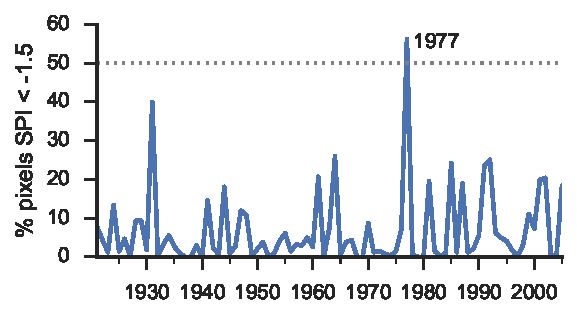
\includegraphics[width=3.13337in]{p3figures/fig_wus_spi_timeseries.pdf}}
\caption{Time series of the percent of pixels in GPCC-derived DJF SPI with values $<$ -1.5 or ``Very Dry'' conditions. The horizontal dotted line indicates the 50\% threshold used to identify extreme widespread dry events, similar to that experienced during 1976 - 1977. These events are associated with anomalously strong coastal ridges while events affecting one-quarter or less of the western US are more commonly associated with ENSO teleconnections.}
\label{fig_wus_spi_timeseries}
\end{figure}

We tested the CESMLE association between extreme widespread events and unusually strong coastal ridge intensity by applying an exact binomial test \citep{3clopper_use_1934, 3conover_practical_1971, 3hollander_nonparametric_1973} to the CESMLE data. We divided the ridge center intensity, in each ensemble member run, into ranked quartiles (i.e. ``Very Weak'', ``Weak'', ``Strong'', ``Very Strong'') and then pooled all ensemble runs together. We then applied a very simple one-sided binomial test ($\alpha = 0.05$) against the null hypothesis that the true probability of an extreme widespread event occurring during a ``Very Strong'' coastal ridge year is 0.25.

\section{Results \& Discussion}

\subsection{Climatology}

\begin{figure}[ht]
\centering
\centerline{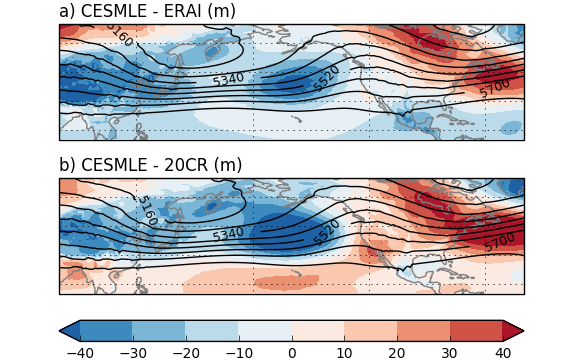
\includegraphics[width=6.5in]{p3figures/fig_z500_climatology.png}}
\caption{CESMLE 500 mb geopotential height climatology and bias. (a) is a comparison between CESMLE and ERAI (1980 - 2005) while (b) compares the CESMLE with 20CR (1920 - 2005). Contours give the CESMLE mean climatology with 60 m intervals. Coloring indicates ensemble-mean bias found by subtracting the ``observed'' reanalysis from the CESMLE mean.}
\label{fig_z500_climatology}
\end{figure}

CESMLE 500 mb geopotential height climatologies are shown in Figure \ref{fig_z500_climatology}. Mean bias relative to the ERA-I (1980 - 2005) is shown as shading in Figure \ref{fig_z500_climatology}a. Mean bias relative to the 20CR (1920-2005) is shown in Figure \ref{fig_z500_climatology}b. Geopotential height fields are usually among the most skillfully simulated products of climate models and reanalysis products \citep[e.g., ][]{3kalnay_ncep/ncar_1996}. The CESMLE mean geopotential height at 500 mb has a few outstanding biases that are relevant to our study. First, The depth of the Aleutian low is generally deeper than shown in both the 20CR and ERA-I. The magnitude-bias for the Aleutian low and other semi-permanent atmospheric circulation anomalies is stronger in the longer 20CR comparison (Figure \ref{fig_z500_climatology}b). This bias suggests that we are likely to see a bias towards more intense ridges, in the discussion below. Note also that the extent of the Aleutian low anomaly is slightly misplaced or expanded, longitudinally, in the central North Pacific Sector.

CESMLE mean precipitation climatologies are shown in Figure \ref{fig_prect_climatology}. Mean bias relative to the GPCP (1980 - 2005) and GPCC (1920 - 2005) is shown in Figures \ref{fig_prect_climatology}a and \ref{fig_prect_climatology}b, and Figures \ref{fig_prect_climatology}c and \ref{fig_prect_climatology}d, respectively. Our comparison with GPCP shows a strong wet bias in CESMLE mean in the western North Pacific and into the eastern North Pacific (Figure \ref{fig_prect_climatology}a). This wet bias in the west North Pacific, near the Kuroshio-Oyashio extension is apparently related to heat and moisture release that enhances localized precipitation and the larger storm track, as has been noted in earlier CMIP5 ensemble studies \citep{3kwon_role_2010, 3choi_uncertainty_2016}. We see this artifact strongly in the CESMLE mean with a wet bias that extends further into the eastern North Pacific. There is also significant dry and wet bias within, and upstream of, the western US. Strong wet bias appears more prevalent, regardless of whether we compare CESMLE to the GPCP or GCPP precipitation fields. The regional bias in the simulations are not surprising because the extreme and complicated North American Cordillera is generally poorly resolved in global climate models. Finer-scale models or downscaling is needed to more accurately simulate important sub-regional precipitation regimes in the western US and Pacific coast.
% * <malevich@email.arizona.edu> 2017-01-16T00:11:10.168Z:
% 
% > Finer-scale models or downscaling
% Maybe can cite examples of this.
% 
% ^.

\begin{figure}[ht]
\centering
\centerline{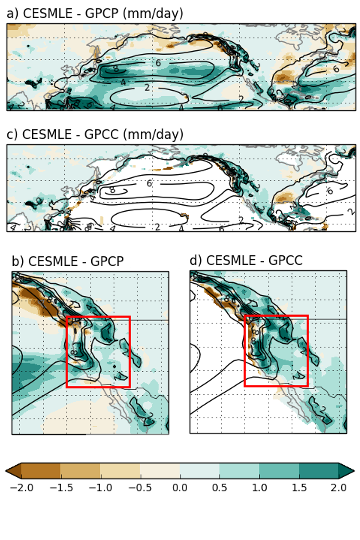
\includegraphics[width=3.5in]{p3figures/fig_prect_climatology.png}}
\caption{Similar to Figure \ref{fig_z500_climatology}, but for precipitation. CESMLE precipitation climatology and bias. (a) and (b) is a comparison between CESMLE and GPCP (1980 - 2005) while (c) and (d) compares the CESMLE with GPCC (1920 - 2005). Contours give the CESMLE mean climatology at 1 mm/day intervals. Coloring indicates ensemble-mean bias found by subtracting the ``observed'' reanalysis from the CESMLE mean climatology. The red box in (b) and (d) is the western US sampling region we use to define extreme widespread events.}
\label{fig_prect_climatology}
\end{figure}

\subsection{Coastal ridge characteristics}

We compare the distribution of winter coastal ridge center position and intensity from the 20CR and CESMLE (1920 - 2005) in Figure \ref{fig_ridge_violins}. As might be expected from the bias in air circulation (Figure \ref{fig_z500_climatology}a and Figure \ref{fig_z500_climatology}b), we find the CESMLE ridges are generally more intense than those in the 20CR (Figure \ref{fig_ridge_violins}a). The upper tail of the center intensity distribution is noticeably heavier than in the 20CR. The center latitude of the ridges also appear biased towards the north, though we see a sharp decrease in the number of ridge centers identified above 55\textdegree~N -- a characteristics also found in the 20CR (Figure \ref{fig_ridge_violins}b). The 20CR has a relatively larger proportion of ridge centers south of 40\textdegree~N latitude while the CESMLE ridges appear more tightly confined around 50\textdegree~N. The CESMLE ridge center longitudes tend to be biased towards the east (Figure \ref{fig_ridge_violins}c). The CESMLE ridge center position bias may relate to the coarsely resolved North American topography in CESMLE simulations.

\begin{figure}[ht]
\centering
\centerline{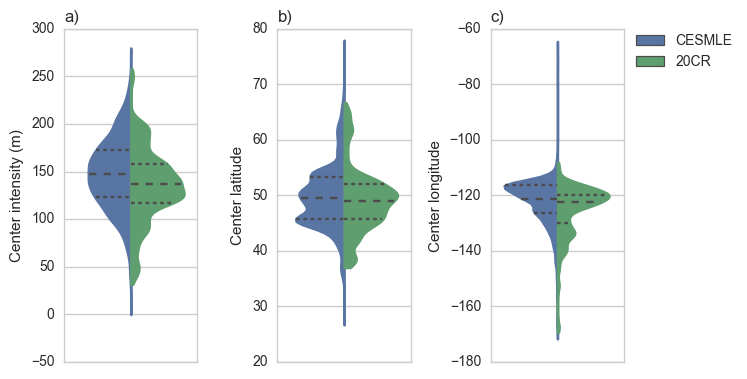
\includegraphics[width=6.5in]{p3figures/fig_ridge_violins.png}}
\caption{Violin plots comparing the distribution of CESMLE (blue) coastal ridge characteristics pooled from all 35 runes with those from 20CR (green) from 1920 - 2005. The characteristics are ridge center intensity (a), ridge center latitude (b), and ridge center longitude (c). Dotted lines indicate distribution quartiles.}
\label{fig_ridge_violins}
\end{figure}

\subsection{Widespread precipitation anomalies}

Plotting the distribution of the proportion of western US gridpoints with SPI $<$ -1.5 (supplemental information Figure \ref{sfig_spi_distribution}) shows that there are few widespread dry events in the observed GPCC data from 1920 - 2005 (supplemental information Figure \ref{sfig_spi_distribution}a), much like we found in Figure \ref{fig_wus_spi_timeseries}. The majority of drought events in the observed historical period do not extend beyond one-quarter of the western US. The 35 CESMLE runs from 1920 - 2005 clearly fill out the tail of this distribution (supplemental information Figure \ref{sfig_spi_distribution}b), with 36 extreme widespread events - events where grid points with SPI $<$ -1.5 cover more than 50\% of the western US. With 3,010 years simulated from 35 model runs, this is a mean frequency of approximately 1.2 extreme widespread events per century or approximately six events per 500 years. The majority of the 35 CESMLE member runs produce at least one extreme widespread dry event in the 85-year period from 1920 - 2005. Twelve ensemble member runs (approximately 34\%) did not produce an extreme widespread dry event and three of the CESMLE runs simulate three extreme widespread events. The maximum number of extreme widespread events simulated in a single member. We find the number of extreme widespread dry events identified is strongly influence by the eastern edge of our western US sampling box. Shifting the eastern edge of the box towards the Pacific coast can greatly increase the number of events found. For example, shifting the edge from 104\textdegree W to 110\textdegree W increases the number of extreme events jumps from 36 to 55. We suspect this %is not a result of reducing the sampling area, but instead
reflects the reduced direct influence of the coastal ridge on the interior and eastern Front Range of the Rockies Mountains \citet[e.g., ][]{3changnon_hydroclimatic_1991, 3malevich_importance_2017}.

A contingency table for western US events in CESMLE shows a relatively even distribution of ridge quartiles during non-extreme widespread dry events (Table \ref{table_contingency}). Extreme widespread events, however, appear to have only occurred during winters with a ``Strong'' or ``Very Strong'' coastal ridge. We find the vast majority of extreme widespread dry events during ``Very Strong'' coastal ridge winters, when ridge intensity is in the upper quartile of its distribution. Our binomial test indicates that the number of ``Very Strong'' ridge and extreme widespread events is significantly higher (30 of 36 events or approximately 83\% of all widespread events) than we might expect by random chance ($p \ll 0.01$). This result shows that CESMLE simulations have a very strong association between high coastal ridge intensity and extreme widespread dry events in the western US. However, it is important to note that extreme widespread events are not a certain outcome from ``Very Strong'' winter ridges in these simulations. We find 705 winters with ``Very Strong'' coastal ridges that did not occur during extreme widespread dry events (Table \ref{table_contingency}).

\begin{table}
\caption{Contingency table giving the number of winters with and without extreme widespread dry event years for given coastal ridge intensity quartile. A binomial test indicates the 36 occurrences of ``Very Strong'' ridges and extreme widespread dry events are significantly higher than we would expect by random chance ($p \ll 0.01$).}
\centering
\begin{tabular}{c c c c c}
\hline
 ~ & \multicolumn{4}{c} {Ridge intensity}\\ \cline{2-5}
  Event & Very Weak & Weak & Strong & Very Strong \\
\hline
 {$not~wide$} & 771  & 737 & 764 & 705 \\
      {$wide$} &   0  &   0 &   6 & *30 \\
\hline
\end{tabular}
\label{table_contingency}
\end{table}

The mean spatial pattern of DJF SPI for the 36 CESMLE-simulated extreme widespread dry events is compared with the observed 1977 event in Figure \ref{fig_widespread_compositemaps}. We find important differences between the observed event and CESMLE mean, but the patterns are surprisingly similar given that the CESMLE, and global climate models generally, have such a prominent precipitation bias in the western US (Figure \ref{fig_prect_climatology}). The CESMLE event-mean (Figure \ref{fig_widespread_compositemaps}a) is clearly weaker and more diffuse than the observed 1977 SPI (Figure \ref{fig_widespread_compositemaps}b), but keep in mind that the CESM field is an average of 36 events. The CESMLE on average also has drier anomalies in the Great Plains and Upper Missouri River basin. Another important difference in the CESMLE is the weaker dry anomalies focused in the Norther Rockies and Pacific Northwest. These areas correspond with a wet-bias in the CESMLE climatology (Figure \ref{fig_prect_climatology}b and Figure \ref{fig_prect_climatology}d), suggesting that the difference between the extreme-event average and 1977 may be mechanistically linked with the subregion's more general precipitation bias in the CESMLE. This bias might be remedied in a statistical or model downscaling of the CESMLE runs.

Individual plots of the 36 events are found in supplemental information Figure \ref{sfig_cesm_allevents}. We measured the spatial similarity of these individual events to the observed 1976 - 1977 event calculating the reflective correlation coefficient (see supplemental information Text 1) between the GPCC DJF SPI in 1976 - 1977 and each of the extreme widespread events identified in CESMLE. The pattern with the least similarity generally shows wet anomalies in the Pacific Northwest, though this is not a common spatial pattern in the CESMLE events (supplemental information Figure \ref{sfig_cesm_allevents}).

\begin{figure}[ht]
\centering
\centerline{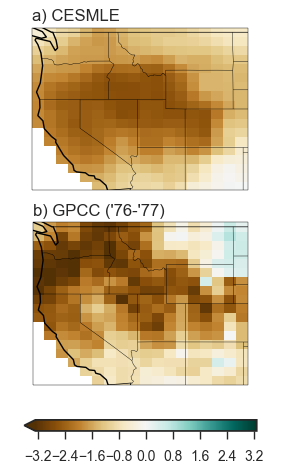
\includegraphics[width=19pc]{p3figures/fig_widespread_compositemaps.png}}
\caption{SPI Composite map of the 36 extreme widespread dry events identified in the 35 CESMLE runs (a) from 1920 - 2005. This is compared with the single, observed, 1977 extreme widespread event. Coloring indicates DJF SPI values. Note that the extreme dry values in (b) extend beyond the colorbar.}
\label{fig_widespread_compositemaps}
\end{figure}

\section{Conclusion}

We examine CESMLE-simulated wintertime precipitation in the western US, and North Pacific coastal ridge characteristics to determine whether the CESMLE simulates extreme widespread dry events, comparable to the 1976 - 1977 drought. We find the CESMLE (35 runs from 1920 - 2005) simulates an average of 6 events every 500 years or 1.2 events every 100 years, though several ensemble members produced as many as three events in a century. The widespread events in the CESMLE are strongly and significantly linked with anomalously intense coastal ridges near the Pacific Northwest coast. On a regional-scale, the simulated events capture the general spatial pattern of the 1977 drought but with several important exceptions, including a mean underestimation of dry anomalies in the northern US Rocky Mountains and Pacific Northwest. These areas correspond with a precipitation bias in the CESMLE simulations that we find when comparing with ``observed'' historical precipitation datasets. We believe these bias might be addressed in a downscaled large ensemble with better-resolved topographic features. We find the ridges in these simulations are generally more intense than those in the historical record. The ridges also have a slight spatial bias in their center position. By examining the ability of CESMLE to replicate extreme and widespread drought events, these results helps stakeholders and water management agencies develop risk assessments for present and future western US water supplies that begin to explicitly account for uncertainty relating to internal climate variability \citep{3reclamation_bureau_of_reclamation_west-wide_2016}.

\section{Acknowledgments}

Thanks to Joellen Russell, Elizabeth Ritchie, Chris Castro, Kevin Anchukaitis, Andrew Comrie, and Dave Meko. Thanks also to our anonymous reviewers for their feedback. NOAA-CIRES Twentieth Century Reanalysis were provided by the NOAA/OAR/ESRL PSD, Boulder, Colorado, USA (http://www.esrl.noaa.gov/psd/). An allocation of computer time from the UA Research Computing High Performance Computing (HPC) and High Throughput Computing (HTC) at the University of Arizona is gratefully acknowledged. This research was supported by the US Bureau of Reclamation WaterSmart program (Agreement \# R11 AP 81 457).

% \bibliographystyle{ametsoc2014}
% \bibliography{references}


\begin{thebibliography}{}
\providecommand{\natexlab}[1]{#1}
\expandafter\ifx\csname urlstyle\endcsname\relax
  \providecommand{\doi}[1]{doi:\discretionary{}{}{}#1}\else
  \providecommand{\doi}{doi:\discretionary{}{}{}\begingroup
  \urlstyle{rm}\Url}\fi

\bibitem[{\textit{Adler et~al.}(2003)\textit{Adler, Huffman, Chang, Ferraro,
  Xie, Janowiak, Rudolf, Schneider, Curtis, Bolvin, Gruber, Susskind, Arkin,
  and Nelkin}}]{3adler_version-2_2003}
Adler, R.~F., G.~J. Huffman, A.~Chang, R.~Ferraro, P.-P. Xie, J.~Janowiak,
  B.~Rudolf, U.~Schneider, S.~Curtis, D.~Bolvin, A.~Gruber, J.~Susskind,
  P.~Arkin, and E.~Nelkin (2003), The {Version}-2 {Global} {Precipitation}
  {Climatology} {Project} ({GPCP}) {Monthly} {Precipitation} {Analysis}
  (1979-{Present}), \textit{J. Hydrometeor.}, \textit{4}(6), 1147--1167,
  \doi{10.1175/1525-7541(2003)004<1147:TVGPCP>2.0.CO;2}.

\bibitem[{\textit{Changnon et~al.}(1991)\textit{Changnon, McKee, and
  Doesken}}]{3changnon_hydroclimatic_1991}
Changnon, D., T.~B. McKee, and N.~J. Doesken (1991), Hydroclimatic variability
  in the {Rocky} {Mountains}, \textit{J Am Water Resources Assoc},
  \textit{27}(5), 733--743, \doi{10.1111/j.1752-1688.1991.tb01471.x}.

\bibitem[{\textit{Choi et~al.}(2016)\textit{Choi, Lu, Son, Frierson, and
  Yoon}}]{3choi_uncertainty_2016}
Choi, J., J.~Lu, S.-W. Son, D.~M.~W. Frierson, and J.-H. Yoon (2016),
  Uncertainty in future projections of the {North} {Pacific} subtropical high
  and its implication for {California} winter precipitation change, \textit{J.
  Geophys. Res. Atmos.}, \textit{121}(2), 2015JD023,858,
  \doi{10.1002/2015JD023858}.

\bibitem[{\textit{Clopper and Pearson}(1934)}]{3clopper_use_1934}
Clopper, C.~J., and E.~S. Pearson (1934), The use of {Confidence} or {Fiducial}
  {Limits} {Illustrated} in the {Case} of the {Binomial}., \textit{Biometrika},
  \textit{26}(4), 404--413, \doi{10.1093/biomet/26.4.404}.

\bibitem[{\textit{Compo et~al.}(2011)\textit{Compo, Whitaker, Sardeshmukh,
  Matsui, Allan, Yin, Gleason, Vose, Rutledge, Bessemoulin, Brönnimann,
  Brunet, Crouthamel, Grant, Groisman, Jones, Kruk, Kruger, Marshall, Maugeri,
  Mok, Nordli, Ross, Trigo, Wang, Woodruff, and Worley}}]{3compo_twentieth_2011}
Compo, G.~P., J.~S. Whitaker, P.~D. Sardeshmukh, N.~Matsui, R.~J. Allan,
  X.~Yin, B.~E. Gleason, R.~S. Vose, G.~Rutledge, P.~Bessemoulin,
  S.~Brönnimann, M.~Brunet, R.~I. Crouthamel, A.~N. Grant, P.~Y. Groisman,
  P.~D. Jones, M.~C. Kruk, A.~C. Kruger, G.~J. Marshall, M.~Maugeri, H.~Y. Mok,
  Ã.~Nordli, T.~F. Ross, R.~M. Trigo, X.~L. Wang, S.~D. Woodruff, and S.~J.
  Worley (2011), The {Twentieth} {Century} {Reanalysis} {Project},
  \textit{Q.J.R. Meteorol. Soc.}, \textit{137}(654), 1--28,
  \doi{10.1002/qj.776}.

\bibitem[{\textit{Conover}(1971)}]{3conover_practical_1971}
Conover, W.~J. (1971), Practical nonparametric statistics, in \textit{Practical
  nonparametric statistics}, pp. 97--104, Wiley, New York.

\bibitem[{\textit{Cousty et~al.}(2009)\textit{Cousty, Bertrand, Najman, and
  Couprie}}]{3cousty_watershed_2009}
Cousty, J., G.~Bertrand, L.~Najman, and M.~Couprie (2009), Watershed {Cuts}:
  {Minimum} {Spanning} {Forests} and the {Drop} of {Water} {Principle},
  \textit{IEEE Transactions on Pattern Analysis and Machine Intelligence},
  \textit{31}(8), 1362--1374, \doi{10.1109/TPAMI.2008.173}.

\bibitem[{\textit{Dawson}(2016)}]{3dawson_eofs_2016}
Dawson, A. (2016), eofs: {A} {Library} for {EOF} {Analysis} of
  {Meteorological}, {Oceanographic}, and {Climate} {Data}, \textit{Journal of
  Open Research Software}, \textit{4}(1), \doi{10.5334/jors.122}.

\bibitem[{\textit{Dee et~al.}(2011)\textit{Dee, Uppala, Simmons, Berrisford,
  Poli, Kobayashi, Andrae, Balmaseda, Balsamo, Bauer, Bechtold, Beljaars,
  van~de Berg, Bidlot, Bormann, Delsol, Dragani, Fuentes, Geer, Haimberger,
  Healy, Hersbach, Hólm, Isaksen, Kållberg, Köhler, Matricardi, McNally,
  Monge-Sanz, Morcrette, Park, Peubey, de~Rosnay, Tavolato, Thépaut, and
  Vitart}}]{3dee_era-interim_2011}
Dee, D.~P., S.~M. Uppala, A.~J. Simmons, P.~Berrisford, P.~Poli, S.~Kobayashi,
  U.~Andrae, M.~A. Balmaseda, G.~Balsamo, P.~Bauer, P.~Bechtold, A.~C.~M.
  Beljaars, L.~van~de Berg, J.~Bidlot, N.~Bormann, C.~Delsol, R.~Dragani,
  M.~Fuentes, A.~J. Geer, L.~Haimberger, S.~B. Healy, H.~Hersbach, E.~V. Hólm,
  L.~Isaksen, P.~Kållberg, M.~Köhler, M.~Matricardi, A.~P. McNally, B.~M.
  Monge-Sanz, J.-J. Morcrette, B.-K. Park, C.~Peubey, P.~de~Rosnay,
  C.~Tavolato, J.-N. Thépaut, and F.~Vitart (2011), The {ERA}-{Interim}
  reanalysis: configuration and performance of the data assimilation system,
  \textit{Q.J.R. Meteorol. Soc.}, \textit{137}(656), 553--597,
  \doi{10.1002/qj.828}.

\bibitem[{\textit{Dettinger et~al.}(2015)\textit{Dettinger, Udall, and
  Georgakakos}}]{3dettinger_western_2015}
Dettinger, M., B.~Udall, and A.~Georgakakos (2015), Western water and climate
  change, \textit{Ecological Applications}, \textit{25}(8), 2069--2093,
  \doi{10.1890/15-0938.1}.

\bibitem[{\textit{Digabel and Lantuejoul}(1978)}]{3digabel_iterative_1978}
Digabel, H., and C.~Lantuejoul (1978), Iterative {Algorithms},
  \textit{Proceedings of the 2nd European Symposium Quantitative Analysis of
  Microstructures in Material Science, Biology and Medicine}, pp. 85--89.

\bibitem[{\textit{Held and Soden}(2006)}]{3held_robust_2006}
Held, I.~M., and B.~J. Soden (2006), Robust {Responses} of the {Hydrological}
  {Cycle} to {Global} {Warming}, \textit{J. Climate}, \textit{19}(21),
  5686--5699, \doi{10.1175/JCLI3990.1}.

\bibitem[{\textit{Hollander and Wolfe}(1973)}]{3hollander_nonparametric_1973}
Hollander, M., and D.~A. Wolfe (1973), Nonparametric statistical methods, in
  \textit{Nonparametric statistical methods}, Wiley series in probability and
  mathematical statistics, pp. 15--22, Wiley, New York.

\bibitem[{\textit{Hunter}(2007)}]{3hunter_matplotlib_2007}
Hunter, J.~D. (2007), Matplotlib: {A} 2d {Graphics} {Environment},
  \textit{Computing in Science \& Engineering}, \textit{9}(3), 90--95,
  \doi{10.1109/MCSE.2007.55}.

\bibitem[{\textit{Hurrell et~al.}(2013)\textit{Hurrell, Holland, Gent, Ghan,
  Kay, Kushner, Lamarque, Large, Lawrence, Lindsay, Lipscomb, Long, Mahowald,
  Marsh, Neale, Rasch, Vavrus, Vertenstein, Bader, Collins, Hack, Kiehl, and
  Marshall}}]{3hurrell_community_2013}
Hurrell, J.~W., M.~M. Holland, P.~R. Gent, S.~Ghan, J.~E. Kay, P.~J. Kushner,
  J.-F. Lamarque, W.~G. Large, D.~Lawrence, K.~Lindsay, W.~H. Lipscomb, M.~C.
  Long, N.~Mahowald, D.~R. Marsh, R.~B. Neale, P.~Rasch, S.~Vavrus,
  M.~Vertenstein, D.~Bader, W.~D. Collins, J.~J. Hack, J.~Kiehl, and
  S.~Marshall (2013), The {Community} {Earth} {System} {Model}: {A} {Framework}
  for {Collaborative} {Research}, \textit{Bull. Amer. Meteor. Soc.},
  \textit{94}(9), 1339--1360, \doi{10.1175/BAMS-D-12-00121.1}.

\bibitem[{\textit{{Intergovernmental Panel on Climate
  Change}}(2013)}]{3ipcc_climate_2013}
{Intergovernmental Panel on Climate Change} (Ed.) (2013), \textit{Climate
  {Change} 2013 - {The} {Physical} {Science} {Basis}: {Working} {Group} {I}
  {Contribution} to the {Fifth} {Assessment} {Report} of the
  {Intergovernmental} {Panel} on {Climate} {Change}}, Cambridge University
  Press, Cambridge, \doi{doi:10.1017/CBO9781107415324}.

\bibitem[{\textit{Kalnay et~al.}(1996)\textit{Kalnay, Kanamitsu, Kistler,
  Collins, Deaven, Gandin, Iredell, Saha, White, Woollen, Zhu, Leetmaa,
  Reynolds, Chelliah, Ebisuzaki, Higgins, Janowiak, Mo, Ropelewski, Wang,
  Jenne, and Joseph}}]{3kalnay_ncep/ncar_1996}
Kalnay, E., M.~Kanamitsu, R.~Kistler, W.~Collins, D.~Deaven, L.~Gandin,
  M.~Iredell, S.~Saha, G.~White, J.~Woollen, Y.~Zhu, A.~Leetmaa, R.~Reynolds,
  M.~Chelliah, W.~Ebisuzaki, W.~Higgins, J.~Janowiak, K.~C. Mo, C.~Ropelewski,
  J.~Wang, R.~Jenne, and D.~Joseph (1996), The {NCEP}/{NCAR} 40-{Year}
  {Reanalysis} {Project}, \textit{Bull. Amer. Meteor. Soc.}, \textit{77}(3),
  437--471, \doi{10.1175/1520-0477(1996)077<0437:TNYRP>2.0.CO;2}.

\bibitem[{\textit{Kay et~al.}(2014)\textit{Kay, Deser, Phillips, Mai, Hannay,
  Strand, Arblaster, Bates, Danabasoglu, Edwards, Holland, Kushner, Lamarque,
  Lawrence, Lindsay, Middleton, Munoz, Neale, Oleson, Polvani, and
  Vertenstein}}]{3kay_community_2014}
Kay, J.~E., C.~Deser, A.~Phillips, A.~Mai, C.~Hannay, G.~Strand, J.~M.
  Arblaster, S.~C. Bates, G.~Danabasoglu, J.~Edwards, M.~Holland, P.~Kushner,
  J.-F. Lamarque, D.~Lawrence, K.~Lindsay, A.~Middleton, E.~Munoz, R.~Neale,
  K.~Oleson, L.~Polvani, and M.~Vertenstein (2014), The {Community} {Earth}
  {System} {Model} ({CESM}) {Large} {Ensemble} {Project}: {A} {Community}
  {Resource} for {Studying} {Climate} {Change} in the {Presence} of {Internal}
  {Climate} {Variability}, \textit{Bull. Amer. Meteor. Soc.}, \textit{96}(8),
  1333--1349, \doi{10.1175/BAMS-D-13-00255.1}.

\bibitem[{\textit{Kwon et~al.}(2010)\textit{Kwon, Alexander, Bond, Frankignoul,
  Nakamura, Qiu, and Thompson}}]{3kwon_role_2010}
Kwon, Y.-O., M.~A. Alexander, N.~A. Bond, C.~Frankignoul, H.~Nakamura, B.~Qiu,
  and L.~A. Thompson (2010), Role of the {Gulf} {Stream} and
  {Kuroshio}–{Oyashio} {Systems} in {Large}-{Scale} {Atmosphere}–{Ocean}
  {Interaction}: {A} {Review}, \textit{J. Climate}, \textit{23}(12),
  3249--3281, \doi{10.1175/2010JCLI3343.1}.

\bibitem[{\textit{Langenbrunner et~al.}(2015)\textit{Langenbrunner, Neelin,
  Lintner, and Anderson}}]{3langenbrunner_patterns_2015}
Langenbrunner, B., J.~D. Neelin, B.~R. Lintner, and B.~T. Anderson (2015),
  Patterns of {Precipitation} {Change} and {Climatological} {Uncertainty} among
  {CMIP}5 {Models}, with a {Focus} on the {Midlatitude} {Pacific} {Storm}
  {Track}, \textit{J. Climate}, \textit{28}(19), 7857--7872,
  \doi{10.1175/JCLI-D-14-00800.1}.

\bibitem[{\textit{Lu et~al.}(2007)\textit{Lu, Vecchi, and
  Reichler}}]{3lu_expansion_2007}
Lu, J., G.~A. Vecchi, and T.~Reichler (2007), Expansion of the {Hadley} cell
  under global warming, \textit{Geophys. Res. Lett.}, \textit{34}(6), L06,805,
  \doi{10.1029/2006GL028443}.

\bibitem[{\textit{Malevich and Woodhouse}(2017)}]{3malevich_importance_2017}
Malevich, S., and C.~Woodhouse (2017), The importance of coastal {Pacific}
  ridge and {Aleutian} low position and intensity for widespread interannual
  anomalies in western {US} streamflow, \textit{J. Clim.}, \textit{In prep.}

\bibitem[{\textit{Manabe and Wetherald}(1975)}]{3manabe_effects_1975}
Manabe, S., and R.~T. Wetherald (1975), The {Effects} of {Doubling} the {CO}2
  {Concentration} on the climate of a {General} {Circulation} {Model},
  \textit{J. Atmos. Sci.}, \textit{32}(1), 3--15,
  \doi{10.1175/1520-0469(1975)032<0003:TEODTC>2.0.CO;2}.

\bibitem[{\textit{McKee et~al.}(1993)\textit{McKee, Doesken, and
  Kleist}}]{3mckee_relationship_1993}
McKee, T.~B., N.~J. Doesken, and J.~Kleist (1993), The relationship of drought
  frequency and druration to time scales, in \textit{Proceedings of the 8th
  {Conference} on {Applied} {Climatology}}, \textit{22}, vol.~17, pp. 179--183,
  American Meteorolical Society, Boston, MA.

\bibitem[{\textit{Reclamation}(2016)}]{3reclamation_bureau_of_reclamation_west-wide_2016}
{Reclamation (Bureau of Reclamation)} (2016), West-{Wide} {Climate} {Risk} {Assessments}:
  {Hydroclimate} {Projections}, \textit{Technical {Memorandum}
  86-68210-2016-01}, U.S. Bureau of Reclamation, Denver, Colorado.

\bibitem[{\textit{Scheff and
  Frierson}(2012)}]{3scheff_twenty-first-century_2012}
Scheff, J., and D.~Frierson (2012), Twenty-{First}-{Century} {Multimodel}
  {Subtropical} {Precipitation} {Declines} {Are} {Mostly} {Midlatitude}
  {Shifts}, \textit{J. Climate}, \textit{25}(12), 4330--4347,
  \doi{10.1175/JCLI-D-11-00393.1}.

\bibitem[{\textit{Schneider et~al.}(2015)\textit{Schneider, Becker, Finger,
  Meyer-Christoffer, Rudolf, and Ziese}}]{3schneider_gpcc_2015}
Schneider, U., A.~Becker, P.~Finger, A.~Meyer-Christoffer, B.~Rudolf, and
  M.~Ziese (2015), {GPCC} {Full} {Data} {Reanalysis} {Version} 7.0 at 0.5
  degrees: {Monthly} {Land}-{Surface} {Precipitation} from {Rain}-{Gauges}
  built on {GTS}-based and {Historic} {Data}.

\bibitem[{\textit{van~der Walt et~al.}(2011)\textit{van~der Walt, Colbert, and
  Varoquaux}}]{3van_der_walt_numpy_2011}
van~der Walt, S., S.~C. Colbert, and G.~Varoquaux (2011), The {NumPy} {Array}:
  {A} {Structure} for {Efficient} {Numerical} {Computation}, \textit{Computing
  in Science \& Engineering}, \textit{13}(2), 22--30,
  \doi{10.1109/MCSE.2011.37}.

\bibitem[{\textit{Vincent and Soille}(1991)}]{3vincent_watersheds_1991}
Vincent, L., and P.~Soille (1991), Watersheds in digital spaces: an efficient
  algorithm based on immersion simulations, \textit{IEEE Transactions on
  Pattern Analysis and Machine Intelligence}, \textit{13}(6), 583--598,
  \doi{10.1109/34.87344}.

\end{thebibliography}

\chapter{Supplementary Information for Extreme widespread Western US precipitation anomalies and wintertime Pacific coast atmospheric ridges in the CESM Large Ensemble historical simulations}

% \section*{Contents}
% %%%Remove or add items as needed%%%
% \begin{enumerate}
% \item Figures S1 to S2
% \end{enumerate}

% \section*{Introduction}

\section*{Text S1.}

Sample reflective correlation is a variation of the common Pearson correlation coefficient that does not center the sample data around a mean value. The sample reflective correlation, $rr_{xy,w}$, between two series, $x$ and $y$, and an optional weight, $w$, is then
\begin{equation}
rr_{xy,w} = \frac{
\displaystyle\sum w_i \cdot x_i \cdot y_i}{\sqrt{(
\displaystyle\sum w_i \cdot x^{2}_i) ~ (
\displaystyle\sum w_i \cdot y^{2}_i})}
\end{equation}
We avoid recentering the CESMLE extreme event fields when comparing with the observed extreme event because we are comparing events from an SPI series, which is already a standardization of precipitation from each model run.

\begin{figure}[ht]
\centering
\centerline{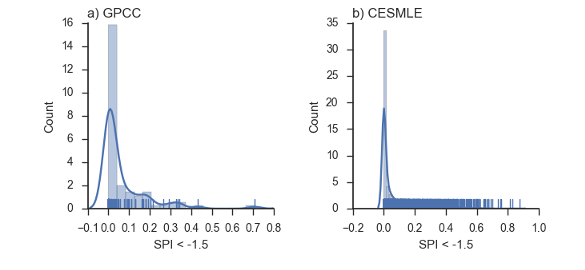
\includegraphics[width=6.5in]{p3figures/fig_spi_distribution.png}}
\caption{Observed (GPCC) distribution/count (a) of the proportion of western US grid points with DJF SPI $<$ -1.5. This is compared with the distribution from the pool of CESMLE runs (b). Plots show count for the plotted histogram and an estimated density function. Plots also include a rug along the x-axis to indicate individual observations. Note that the extreme ends of the tail in the GPCC distribution are considerably more filled-out in the ensemble simulations of (b).}
\label{sfig_spi_distribution}
\end{figure}

\begin{figure}[ht]
\centering
\centerline{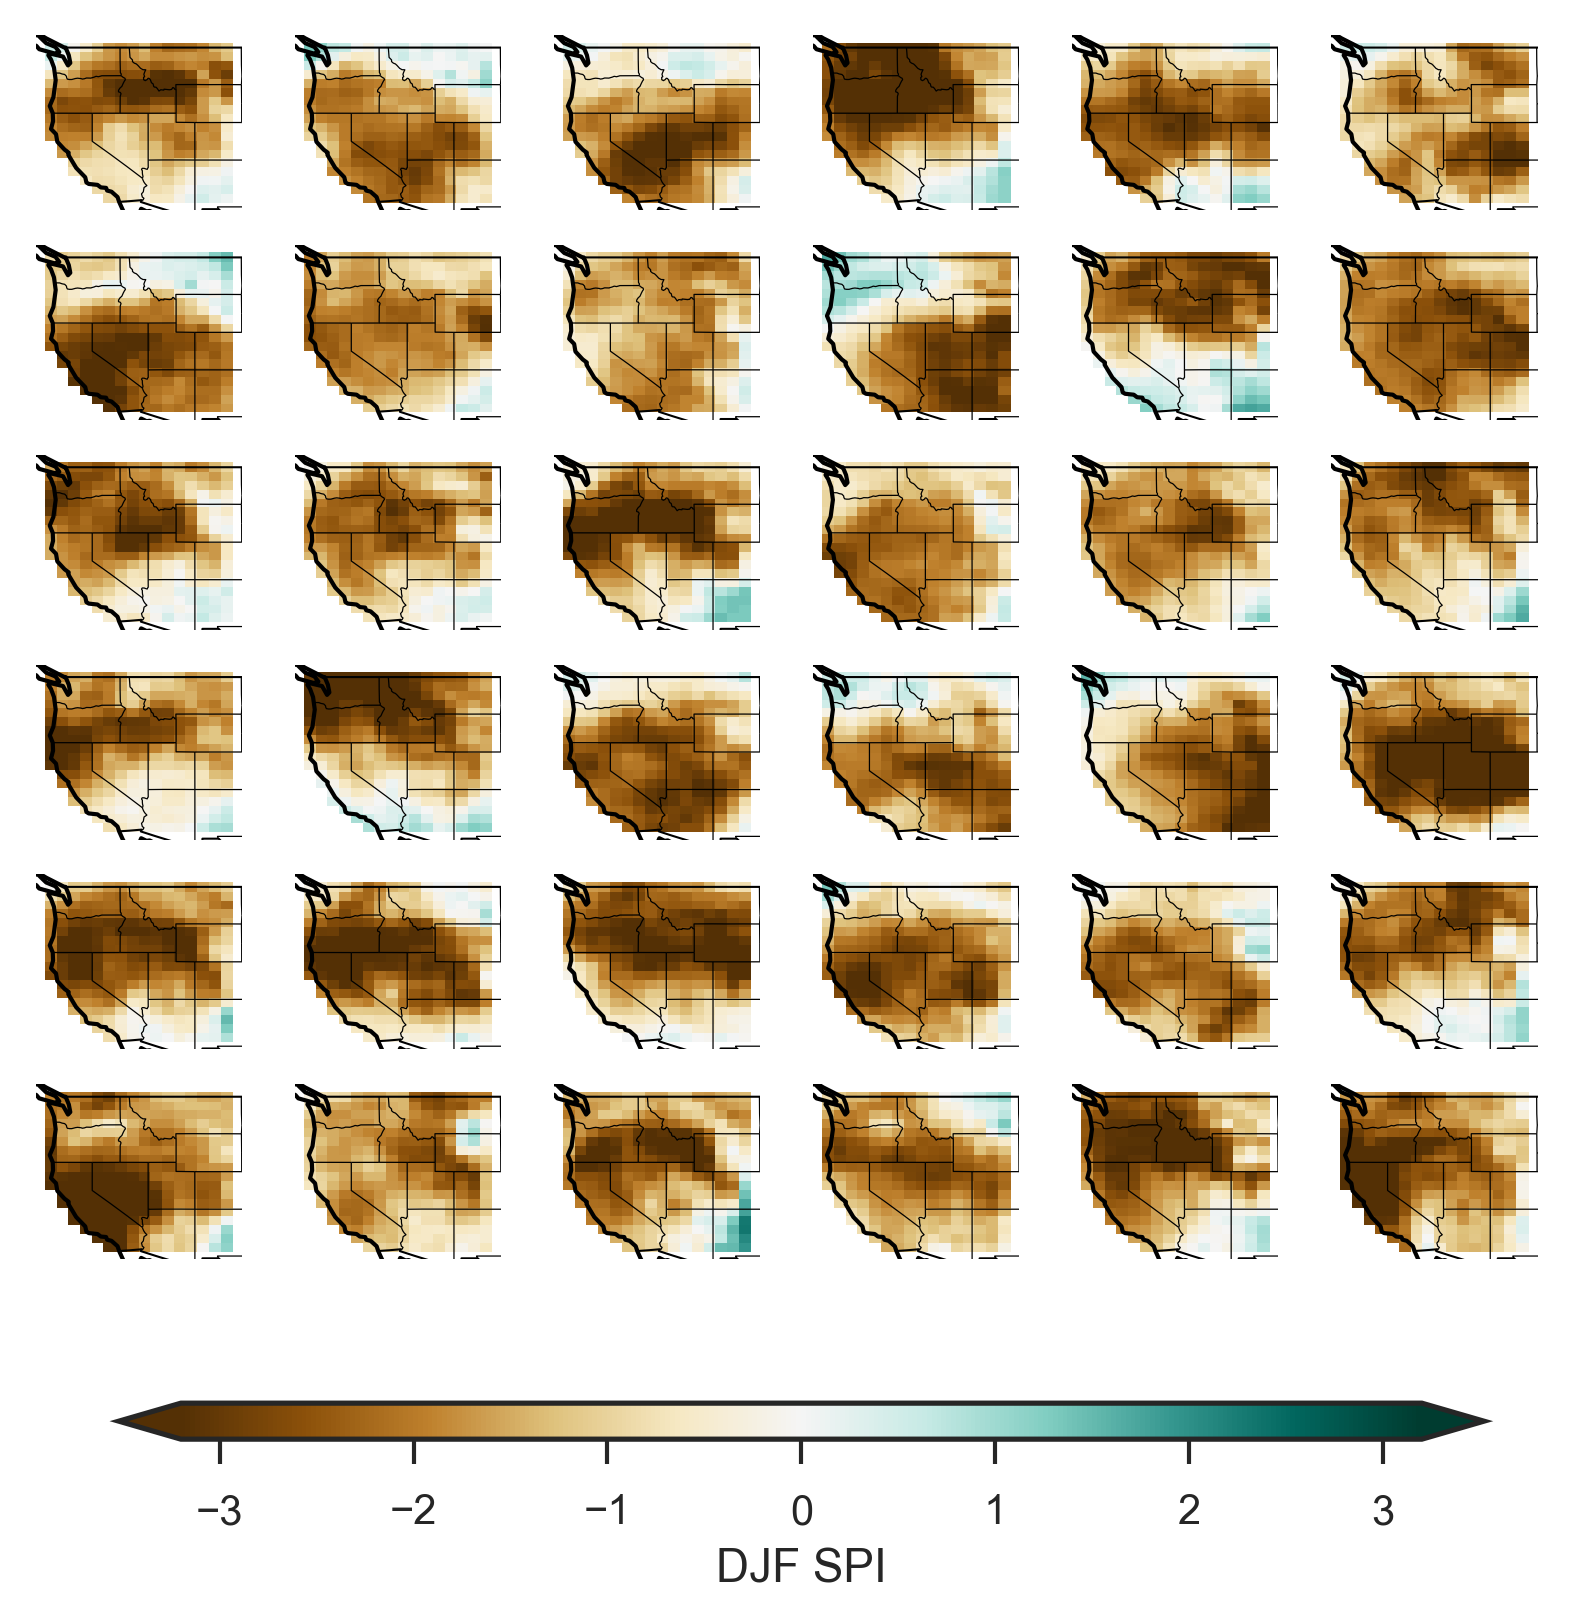
\includegraphics[width=39pc]{p3figures/fig_cesm_allevents.png}}
\caption{Western US DJF SPI for all ``extreme widespread events'' identified in the CESMLE. The color scale used in this image is the same as that used in Figure \ref{fig_widespread_compositemaps}}
\label{sfig_cesm_allevents}
\end{figure}


% Use this manual as a guide for setting up the physical format of your
% thesis, dissertation or document. Your thesis will represent you, your
% department, and The University of Arizona in the international scholarly
% community. Your work is important and worthy of professional presentation.
% This manual lists Graduate College requirements for the mechanical aspects
% of meeting these high standards.

% In this manual the word thesis, includes documents and dissertations. If
% format requirements for the document or dissertation vary from those for the
% thesis, specific requirements for each type of paper will be listed.

% Two final copies of the thesis must be submitted; both must meet all
% specifications of this manual. The two final copies should be submitted
% unbound in a box to the Graduate College Degree Certification Office.

% \chapter{University Microfilms Incorporated (UMI)}

% Your thesis will be published by University Microfilms Incorporated, Ann
% Arbor, Michigan. Upon certification by your major professor, your examining
% committee, and the Graduate College, a copy of the thesis and a Special
% Abstract are forwarded to UMI. The manuscript is cataloged and microfilmed,
% the microfilm negative is inspected and put in vault storage. Paper copies
% of your work will be produced on demand by UMI. Catalog information is sent
% to the Library of Congress for production and distribution of catalog cards
% for libraries. The original copy of the thesis is returned to The University
% of Arizona Library. The Special Abstract is printed in Microfilm Abstracts
% and distributed to leading libraries in the United States and abroad and to
% a selected list ofjournals and abstracting services.

% Publication by UMI does not preclude publication by other means later. You
% are urged to submit your work for publication in a scholarly or professional
% journal. Suitable acknowledgment must indicate that the publication is a
% thesis, dissertation, or document, or portion thereof, which was submitted
% in partial fulfillment of the requirements for a degree at the University of
% Arizona.

% You must complete a UMI publication agreement, available through the Degree
% Certification Office.


% \chapter{General Format Requirements}

% \section{Margins}

% Text, illustrations (figures) or tables must not appear outside the
% specified margins. Specific margin requirements are listed in ORDER OF
% SECTIONS under each category. Page numbers are the only item which may
% appear outside the margin requirements.

% \section{Corrections on Pages}

% Do not use correction fluid or correction tape. These materials flake off in
% handling and storage, exposing the original errors.

% \section{Page numbers}

% The title page is page 1 of the thesis. All pages which follow are numbered
% in a single sequence with arabic numerals. Page numbers must be placed at
% least 1 " below the top of the sheet, and 1" from the right edge. The
% numbers must be at least 1/4" above the first line of text. You may omit the
% printed page number on the title page; all other pages must have printed
% page numbers. Do not use page headers. Do not use the phrase, Page xx; just
% the numeral.

% \section{Paper}

% See Table \ref{t1}.

% \begin{table}
% \hrule
% \begin{tabular*}{\textwidth}{@{}l@{\extracolsep{\fill}}l@{}}
%   1. & Xerox Image Series Smooth Paper \\
%   2. & Xerox Image Elite Paper 25\% Cotton \\
%   3. & Xerox Series 10 \\
%   4. & 100\% Cotton - 20 lb weight \\
%   5. & Cranes Crest Bond - 100\% Cotton Acid Free \\
% \end{tabular*}
% \hrule
% \caption{Required Paper} \label{t1}
% \end{table}
  

% \section{Photocopy Quality}

% Photocopies must meet all requirements for margins, readability, and type of
% paper. This includes all photocopied documents, tables, illustrations and
% appendix pages.

% \section{Printers}

% Laser printing or other letter quality printing is required. Impact, or
% daisy wheel printing is generally acceptable. 24-pin dot matrix near letter
% quality and draft quality printing are not acceptable.

% \section{Type Fonts}

% Standard serif typefaces such as Courier and Times Roman reproduce and
% microfilm well. Do not use modern Sans Serif types, which read well in the
% original but do not reduce well for microfilming. Ornamental styles such as
% Script and Old English may not be used. Limit the use of italic styles to
% standard uses in bibliographic citations and foreign words. Boldface should
% be restricted to very small segments of the text and to infrequent
% occurrences.

% \subsection{Type Size}

% Use 12-point or 14-point for proportional fonts; 10 cpi or 12 cpi for
% non-proportional fonts. A proportional font allows proportional spacing - a
% feature that gives a printed page a more pleasing appearance by allowing for
% different widths of characters. The letter w, for example, is wider than the
% letter i. Normally, when these letters are printed, both are given the same
% amount of space; the result can be gaps that are visually distracting. With
% proportional printing, the letter w is given more space than the letter i,
% creating a more aesthetic and professional-looking line of text.

% \subsection{Typewritten Papers}

% Papers prepared on good quality electric typewriters are acceptable. All
% margin, paper quality, and typographic requirements apply. Type size should
% be Pica (10 cpi) or Elite (12 cpi)


% \chapter{Order of Sections}

% Components of your thesis must be in the following order, formatted as
% specified:

% \begin{enumerate}
%   \item Title Page
%         \begin{itemize}
%         \item Required
%         \item Margins:
%              \begin{itemize}
%              \item Top 2.5"
%              \item Bottom 1.5"
%              \item Left 1.5"
%              \item Right 1"
%              \end{itemize}
%         \item Spacing: Follow sample
%         \end{itemize}
%   \item Final Examining Committee Approval Form
%         \begin{itemize}
%         \item Required for dissertations and music documents, not for theses.
%           The approval form for the thesis is included in the Statement by
%           Author (see item 3 below).
%         \item Note: Before the final oral defense the student obtains the
%           Approval Pages from the Degree Certification Office. Original
%           signatures are required on both final copies.
%         \end{itemize}
%   \item Statement by Author
%         \begin{itemize}
%         \item Required
%         \item Margins:
%              \begin{itemize}
%              \item Top 2.5"
%              \item Bottom 1"
%              \item Left 1.5"
%              \item Right 1"
%              \end{itemize}
%         \item Spacing: Single
%         \item Note: Follow examples. Original signatures are required on both
%           final copies.
%         \end{itemize}
%   \item Acknowledgements
%         \begin{itemize}
%         \item Optional
%         \item Margins: Same as Body of Paper
%         \item Spacing: Maybe single spaced
%         \item Note: One page maximum
%         \end{itemize}
%   \item Dedication
%         \begin{itemize}
%         \item Optional
%         \item Margins: Same as Body of Paper
%         \item Spacing: Must be double spaced
%         \item Note: One page maximum
%         \end{itemize}
%   \item Table of Contents
%         \begin{itemize}
%         \item Required
%         \item Margins: Same as Body of Paper
%         \item Note: See "Notes for Table of Contents" for notes on format.
%         \end{itemize}
%   \item List of Illustrations/List of Tables
%         \begin{itemize}
%         \item Required if document contains illustrations, figures or tables.
%         \item Margins: Same as Body of Paper
%         \item Note: Formatted like Table of Contents; see "Notes for List of
%           Illustrations / List of Tables" for more information.
%         \end{itemize}
%   \item Abstract
%         \begin{itemize}
%         \item Required
%         \item Margins:
%              \begin{itemize}
%              \item Top 1.5"
%              \item Bottom 1"
%              \item Left 1.5"
%              \item Right 1"
%              \end{itemize}
%         \item Spacing: Double spaced
%         \item Note: A Special Abstract for UMI is also required. The text
%           remains the same for both versions, but formatting requirements
%           differ. See "Abstract and Special Abstract Compared".
%         \end{itemize}
%   \item Body of Paper
%         \begin{itemize}
%         \item Required
%         \item Margins:
%              \begin{itemize}
%              \item Top 1.5"
%              \item Bottom 1"
%              \item Left 1.5"
%              \item Right 1"
%              \end{itemize}
%         \item Spacing: Double, except for long quotations, footnotes, table and
%           illustration captions
%         \item Note: Begin each major section on a new page. Margin requirements
%           apply to every page of the thesis unless otherwise specified in
%           this manual. See APPENDIX A, INCLUSION OF PUBLISHED PAPERS OR
%           MANUSCRIPTS FOR PUBLICATION, if your department allows this
%           option.
%         \end{itemize}
%  \item Appendices
%         \begin{itemize}
%         \item Optional
%         \item Margins: Same as Body of Paper
%         \item Spacing: Depends on nature of Appendix material
%         \item Note: Each Appendix must begin on a new page.
%         \end{itemize}
%  \item References
%         \begin{itemize}
%         \item Required if citations are used
%         \item Margins: Same as Body of Paper
%         \item Spacing: Citations single spaced; double space between citations
%         \item Note: Use your department's preferred citation style; consult with
%           your advisor if more than one style is acceptable. Title this
%           section REFERENCES or WORKS CITED. Do not use the word,
%           Bibliography.
%         \end{itemize}
% \end{enumerate}

% \section{Sample Title Page}

% Margins:
% \begin{itemize}
%    \item Top 2.5"
%    \item Bottom 1.5"
%    \item Left 1.5"
%    \item Right 1"
%    \item The title page is centered within the left and right margins.
% \end{itemize}
% Title in capital letters:
% \begin{verbatim}
%                SEBASTIEN CASTELLIO, APOSTLE OF TOLERANCE

%                        IN THE SIXTEENTH CENTURY
% \end{verbatim}
% Use your full name, spelled out:
% \begin{verbatim}
%                                   by

%                           Jane Allison Smith
% \end{verbatim}
% This rule (solid line) is 2" long and is placed approximately 5" below the
% top of the page. Copyright statement, if used, is placed directly below the
% rule:
% \begin{verbatim}
%                        _____________________
%                 Copyright (c) Jane Allison Smith 1992
% \end{verbatim}
% Follow the capitalization and spacing of the lines in the bottom section:
% \begin{verbatim}
%              A Thesis Submitted to the Faculty of the

%                  DEPARTMENT OF ROMANCE LANGUAGES

%            In Partial Fulfillment of the Requirements
%                        For the Degree of

%                         MASTER OF ARTS
%                    WITH A MAJOR IN SPANISH

%                    In the Graduate College

%                   THE UNIVERSITY OF ARIZONA

%                            1 9 9 2
% \end{verbatim}

% \subsection{Notes}

% This is a sample page for a THESIS. For a doctoral degree substitute
% DISSERTATION for THESIS; for a musical arts degree, substitute DOCUMENT for
% THESIS. Substitute DOCTOR OF PHILOSOPHY, DOCTOR OF MUSICAL ARTS, or other
% title as appropriate.

% The statement, WITH A MAJOR IN..., is included only if the name of the major
% field of study is not exactly the same as the official name of the
% department

% Put spaces between the digits of the year: 1 (space) 9 (space) 9 (space) 2

% In its entirety, see Figure \ref{f1}
% \begin{figure}
% \hrule
% \begin{verbatim}

%                SEBASTIEN CASTELLIO, APOSTLE OF TOLERANCE

%                        IN THE SIXTEENTH CENTURY

%                                   by

%                           Jane Allison Smith

%                        _____________________
%                 Copyright © Jane Allison Smith 1992

%              A Thesis Submitted to the Faculty of the

%                  DEPARTMENT OF ROMANCE LANGUAGES

%            In Partial Fulfillment of the Requirements
%                        For the Degree of

%                         MASTER OF ARTS
%                    WITH A MAJOR IN SPANISH

%                    In the Graduate College

%                   THE UNIVERSITY OF ARIZONA

%                            1 9 9 2

% \end{verbatim}
% \hrule
% \caption{Example Title Page}\label{f1}
% \end{figure}


% \subsection{Copyrighting the Thesis or Dissertation}

% Copyrighting of a thesis is optional. Publication by University Microfilms
% does not preclude publication by other methods later. If you want University
% Microfilms Incorporated to file, on your behalf, an application for
% registration of a claim of copyright on your manuscript, you must indicate
% this on the agreement form you complete for UMI and submit the required fee
% by certified check or money order. This service includes payment of the
% registration fee, preparation of the application, and submission of copies
% required by the Copyright Office.

% The ownership of a copyright shall reside with the student unless otherwise
% stated by University policy or by terms of the research grants, fellowships,
% financial aid, etc. which were used to support the student's research.

% Additional information on obtaining a copyright is available from the
% Graduate College Degree Certification Office or the United States Copyright
% Office, Library of Congress, Washington, D. C. 20559.


% \section{Statement by Author}

% Below are four samples of the Statement by Author. Select the applicable
% sample: non-copyrighted thesis, copyrighted thesis, non-copyrighted
% dissertation, or copyrighted dissertation, and copy it. Doctor of Musical
% Arts students must substitute document for thesis or dissertation. For
% theses, substitute the full name of your advisor for the name on the sample
% page, Figures~\ref{f2}, \ref{f3}, \ref{f4}, \ref{f5}.

% Margins:
% \begin{itemize}
%    \item Top 2.5"
%    \item Bottom 1.5"
%    \item Left 1.5"
%    \item Right 1"
% \end{itemize}


% \begin{figure}
% \hrule
% \begin{verbatim}

%                  STATEMENT BY AUTHOR

%    This thesis has been submitted in partial fulfillment of
% requirements for an advanced degree at The University of
% Arizona and is deposited in the University Library to be
% made available to borrowers under rules of the Library.

%    Brief quotations from this thesis are allowable without
% special permission, provided that accurate acknowledgment of
% source is made.  Requests for permission for extended
% quotation from or reproduction of this manuscript in whole
% or in part may be granted by the head of the major
% department or the Dean of the Graduate College when in his
% or her judgment the proposed use of the material is in the
% interests of scholarship.  In all other instances, however,
% permission must be obtained from the author.

%                      SIGNED: ________________________________

%                APPROVAL BY THESIS DIRECTOR

%   This thesis has been approved on the date shown below:

% _________________________________  _________________________
%          Jane M. Doe                        Date
%    Professor of Chemistry

% \end{verbatim}
% \hrule
% \caption{Non-copyrighted thesis} \label{f2}
% \end{figure}

% \begin{figure}
% \hrule
% \begin{verbatim}

%                  STATEMENT BY AUTHOR

%    This thesis has been submitted in partial fulfillment of
% requirements for an advanced degree at The University of
% Arizona and is deposited in the University Library to be
% made available to borrowers under rules of the Library.

%    Brief quotations from this thesis are allowable without
% special permission, provided that accurate acknowledgment of
% source is made.  Requests for permission for extended
% quotation from or reproduction of this manuscript in whole
% or in part may be granted by the copyright holder.

%                      SIGNED: ________________________________

%                APPROVAL BY THESIS DIRECTOR

%   This thesis has been approved on the date shown below:

% _________________________________  _________________________
%          Jane M. Doe                        Date
%    Professor of Chemistry

% \end{verbatim}
% \hrule
% \caption{Copyrighted thesis} \label{f3}
% \end{figure}

% \begin{figure}
% \hrule
% \begin{verbatim}

%                  STATEMENT BY AUTHOR

%    This dissertation has been submitted in partial
% fulfillment of requirements for an advanced degree at The
% University of Arizona and is deposited in the University
% Library to be made available to borrowers under rules of the
% Library.

%    Brief quotations from this dissertation are allowable
% without special permission, provided that accurate
% acknowledgment of source is made.  Requests for permission
% for extended quotation from or reproduction of this
% manuscript in whole or in part may be granted by the head of
% the major department or the Dean of the Graduate College
% when in his or her judgment the proposed use of the material
% is in the interests of scholarship.  In all other instances,
% however, permission must be obtained from the author.

%                      SIGNED: ________________________________

% \end{verbatim}
% \hrule
% \caption{Non-copyrighted dissertation} \label{f4}
% \end{figure}


% \begin{figure}
% \hrule
% \begin{verbatim}

%                  STATEMENT BY AUTHOR

%    This dissertation has been submitted in partial
% fulfillment of requirements for an advanced degree at The
% University of Arizona and is deposited in the University
% Library to be made available to borrowers under rules of the
% Library.

%    Brief quotations from this dissertation are allowable
% without special permission, provided that accurate
% acknowledgment of source is made.  Requests for permission
% for extended quotation from or reproduction of this
% manuscript in whole or in part may be granted by the copyright
% holder.

%                      SIGNED: ________________________________

% \end{verbatim}
% \hrule
% \caption{Copyrighted dissertation}\label{f5}
% \end{figure}


% \section{Notes for Table of Contents}

% The Table of Contents is required. All levels of subheadings in your
% manuscript must appear in the Table of Contents. The TABLE OF CONTENTS for
% this Manual contains two levels; your table of contents might contain more.

% Margins:
% \begin{itemize}
%    \item Top 1.5"
%    \item Bottom 1"
%    \item Left 1.5"
%    \item Right 1"
% \end{itemize}
% Format requirements include:
% \begin{itemize}
%    \item The heading TABLE OF CONTENTS at the top of the first page of this
%      section, and TABLE OF CONTENTS - Continued on each continuation page.
%    \item Page numbers at upper right.
%    \item Dot leaders .......................... from headings to page numbers.
%    \item Indent each level of subheadings 4 spaces from the level above.
%    \item Headings in the Table of Contents must exactly match the headings used
%      in the body of the paper, and should be typographically the same (e.g.,
%      type font and style, capitalization).
%    \item Use all capital letters for major headings. (Subheadings may be upper
%      and lower case.)
%    \item Each Appendix must have its own letter designation and title.
%      Appendices are major divisions. The title appears in caps on the left
%      margin at the same level of importance as chapter headings.
% \end{itemize}
% Format options include:
% \begin{itemize}
%    \item Chapter numbering. You may number your chapters with either arabic or
%      roman numerals.
%    \item Subheading numbers. If chapters are numbered, you may also number
%      subheadings.
% \end{itemize}
% For example, see Figures \ref{f6} and \ref{f7}.

% \begin{figure}
% \hrule
% \begin{verbatim}

%        I. LIST OF TABLES ...............................  6
%       II. INTRODUCTION .................................  8
%               Literature Review ........................  8
%               Statistical Methods ...................... 11

% \end{verbatim}
% \hrule
% \caption{Example 1 for Table of Contents} \label{f6}
% \end{figure}

% \begin{figure}
% \hrule
% \begin{verbatim}

%        1. LIST OF TABLES ...............................  6
%        2. INTRODUCTION .................................  8
%              2.1 Literature Review .....................  8
%              2.2 Statistical Methods ................... 11

% \end{verbatim}
% \hrule
% \caption{Example 2 for Table of Contents} \label{f7}
% \end{figure}

% \section{Notes for List of Illustrations / List of Tables}

% These lists, which resemble the Table of Contents, are required if your
% thesis contains illustrations, figures, graphs or tables. Include a List of
% Illustrations (or List of Figures) for figures, maps and drawings. Include a
% List of Tables for graphs and tables. Illustrations or tables which appear
% in the appendices only may or may not be included with the List of
% Illustrations (or List of Figures) or the List of Tables.

% Material in the List of Illustrations is numbered in sequence, Figure 1,
% Figure 2, etc. You may construct this sequence as you wish, e.g., Figure
% 1.1, 1.2, 2.1, 2.2.... Use LIST OF ILLUSTRATIONS as the title for the first
% page and LIST OF ILLUSTRATIONS - Continued for subsequent pages. You may use
% LIST OF FIGURES instead of LIST OF ILLUSTRATIONS if your department prefers.

% Material in the List of Tables should be given its own separate sequence of
% numbers, Table 1, Table 2, etc. You may also construct this sequence as you
% wish. Use LIST OF TABLES as the title for the first page and LIST OF TABLES
% - Continued for subsequent pages.

% For examples see Figures \ref{f8} and \ref{f9}.
% \begin{figure}
% \hrule
% \begin{verbatim}

%                           LIST OF ILLUSTRATIONS

% FIGURE 1.1, Topographic map of valley ............................. 14
% FIGURE 1.2, View of valley, northwest approach .................... 20
% FIGURE 2.1, Cross section of burial mound ......................... 27
% FIGURE 2.2, Intact jar found near mound ........................... 28

% \end{verbatim}
% \hrule
% \caption{Sample List of Illustrations} \label{f8}
% \end{figure}

% \begin{figure}
% \hrule
% \begin{verbatim}

%                                LIST OF TABLES

% TABLE 1.1, Population estimates, 850-1100 a.d. .................... 16
% TABLE 2.1, Number and type of artifacts compared with nearby sites  29

% \end{verbatim}
% \hrule
% \caption{Sample List of Tables} \label{f9}
% \end{figure}


% \section{Abstract and Special Abstract Compared}

% \subsection{Abstract}

% The Abstract is included as a page of your thesis. It is a numbered page in
% the thesis, appearing just before the main body of the text. The heading
% ABSTRACT is centered at the beginning of the first page. A sample abstract
% page follows (Figure~\ref{f10}). Compare it with the Special Abstract
% sample.

% Margins:
% \begin{itemize}
%    \item Top 1.5"
%    \item Bottom 1"
%    \item Left 1.5"
%    \item Right 1"
% \end{itemize}


% \subsection{Special Abstract}

% The Special Abstract contains the same text as the Abstract, but is
% formatted for microfilming by UMI for Dissertation Abstracts International.
% Treat the Special Abstract as a separate document. Include one copy of the
% Special Abstract and two extra copies of your title page when submitting the
% two final copies of your thesis.

% Note the heading of the Special Abstract sample page which follows. Use the
% thesis title as it appears on your title page. Use your full name, and add
% the appropriate designation for your degree. Include your director's name as
% shown (Figure~\ref{f11}).

% Margins:
% \begin{itemize}
%    \item Top 1.5"
%    \item Bottom 1"
%    \item Left 1.5"
%    \item Right 1"
% \end{itemize}

% \begin{figure}
% \hrule
% \begin{verbatim}

%                           ABSTRACT

%    This is the body of your abstract, limited to 150 words

% for a thesis, and 350 words for a dissertation or document.

% The word count limits apply to the regular Abstract in the

% thesis and to this separate Special Abstract.  Use the same

% text for both; just adjust the margins and heading.  The

% abstract should summarize your work.  The UMI booklet listed

% in the resources section of this Manual (here) provides some

% writing tips.  The abstract for a dissertation or document

% may be longer than one page; word count is more important

% than page length in this section.

%    This version of the Abstract, with simple heading, page

% number, and 1.5" top margin, is included as part of your

% thesis.

% \end{verbatim}
% \hrule
% \caption{Sample Abstract} \label{f10}
% \end{figure}

% \begin{figure}
% \hrule
% \begin{verbatim}

%                       COMPLETE TITLE OF

%             YOUR THESIS, DISSERTATION OR DOCUMENT

%                    Jane Allison Doe, M.S.

%                The University of Arizona, 1992

% Director: John J. Jones

%    This is the body of your abstract, limited to 150 words

% for a thesis, and 350 words for a dissertation or document.

% The word count limits apply to the regular Abstract in the

% thesis and to this separate Special Abstract.  Use the same

% text for both; just adjust the margins and heading.  The

% abstract should summarize your work.  The UMI booklet listed

% in the resources section of this Manual (here) provides some

% writing tips.  The abstract for a dissertation or document

% may be longer than one page; word count is more important

% than page length in this section.

%    This version of the Abstract, with special heading, no

% page number, and 1.5" top margin, is a separate document for

% UMI.  Submit one copy of the special abstract, and two extra

% copies of your title page, in the box with the final copies

% of your thesis.

% \end{verbatim}
% \hrule
% \caption{Sample Special Abstract} \label{f11}
% \end{figure}

% \appendix

% \chapter{Inclusion of Published Papers or Manuscripts for Publication}

% Under a policy adopted by The University of Arizona Graduate Council in
% January, 1992, your department may allow published and publishable papers to
% be included as part of your thesis. The reprints or manuscripts are treated
% as appendices, and the body of your thesis must include a summary of your
% contribution and a summary of the research. The Graduate College will accept
% theses in this format from any unit with an implementation policy on file
% with the Graduate College Degree Certification Office.

% \section{Body of Paper}
%  The ORDER OF SECTIONS applies. In addition, the Body of the
% Paper must include two chapters as follows:
% \begin{enumerate}
%   \item An introduction describing the unique contribution of your work to the
%      field of study. Use the following subsections as appropriate:
%        \begin{enumerate}
%        \item Explanation of the problem and its context
%        \item A review of the literature
%        \item Explanation of thesis format
%           This subsection explains the relationship of the papers included
%           and your contribution to each of the papers; where doctoral
%           research efforts are part of a larger collaborative project, you
%           must be able to identify one aspect of the project as your own and
%           demonstrate an original contribution. Your role in the research
%           and production of the published paper(s) should be clearly
%           specified.
%        \end{enumerate}
%   \item A chapter titled PRESENT STUDY which summarizes the methods, results,
%      and conclusions of the research. The chapter should begin with a
%      statement such as:
% \begin{quote}
%           The methods, results, and conclusions of this study are
%           presented in the papers appended to this thesis. The
%           following is a summary of the most important findings in
%           these papers.
% \end{quote}
% \end{enumerate}

% \section{Appendices}
% All mechanical requirements for Appendices listed in the ORDER
% OF SECTIONS apply. Your appendices will consist of:
% \begin{enumerate}
%   \item A reprint of each paper as a separate appendix in the following
%   order: 
%        \begin{enumerate}
%        \item a copy of the title page of the journal in which the article
%           appeared
%        \item the statement of permission for use of copyrighted material (see
%           Appendix B: Permissions)
%        \item the reprint(s), copied single-sided onto the required type of
%           paper
%        \end{enumerate}
%   \item Supplementary materials such as data tables, graphs, and maps which
%      might ordinarily appear as appendices to a thesis.
% \end{enumerate}
% These two types of appendices form a single sequence, assigned letters and
% titled as described in this manual. All Appendix pages are part of the
% single pagination sequence of the thesis. The page numbers will be typed in
% as needed.


% \chapter{Permissions}

% Use of copyrighted material in your thesis, including illustrations, usually
% requires written permission from the copyright holder. Start this
% time-consuming process as early as possible. Play it safe and assume that
% you must obtain permission if the material is copyrighted. Consult your
% advisor or departmental graduate secretary about this process.

% Exceptions, sometimes pertaining to small fractions of a musical score or
% other document, are governed by the concept of "fair use." Factors weighed
% in determining "fair use" include: the purpose of the use, whether
% commercial or non-profit and educational; the nature of the copyrighted
% work; the amount and substance of the material used in relation to the
% entire work; and the effect of the use upon the potential market for or
% value of the copyrighted work. The "fair use" concept is explained in detail
% in the Chicago Manual of Style. According to the Association of American
% University Presses, permission is required for quotations which are complete
% units, for example, an entire poem, letter, book chapter, or an entire map,
% chart, drawing or other illustration.

% Permission to use copyrighted material should be in writing and retained by
% the author. The release letters should indicate that permission extends to
% microfilming and publication by University Microfilms Incorporated and that
% the copyright owners are aware that UMI may sell, on demand, single copies
% of the thesis, dissertation or document, including the copyrighted
% materials, for scholarly purposes. UMI requires copies of permission letters
% to be attached to the publication agreement, and assumes no liability for
% copyright violations. If permission letters are not supplied, copyrighted
% materials may not be filmed.

% It is polite and good practice to obtain permission to use noncopyrighted
% material, which may or may not be acknowledged in the text.

% For additional information, telephone the Copyright Public Information
% Office in Washington, DC, (202) 479-0700, weekdays between 8:30 a.m. and
% 5:00 p.m. EST or write to the Copyright Office, Library of Congress,
% Washington D.C. 20559.

% \chapter{Human/Animal Subjects Approval}

% Research involving human subjects or live vertebrate animals requires
% permission from the relevant University committee. Consult your research
% director for details. If you are working on a project for which your
% director has obtained the required permissions, be sure your name is listed
% on the protocol approval and that you have the control number of the
% approval in your records.

% Research activities involving the use of human subjects require the review
% and approval of the University Human Subjects Committee. A copy of the Human
% Subjects approval letter along with The Human Subjects Research Statement
% must be in the student's file in the Graduate College Degree Certification
% Office. Questions regarding protocol can be answered by the Human Subjects
% Committee. Their telephone number is (602) 626-6721.

% Research involving any live vertebrate animals must be approved by the
% Institutional Animal Care and Use Committee (IACUC) - The Animal Research
% Protocol Review form must be completed by the student/instructor and
% submitted to the protocol office for review and approval. Contact University
% Animal Care for instructions, forms and protocol. Their telephone number is
% (602) 621-3454

% \chapter{Illustrations, Tables, Graphs}

% Use illustrative material drawn or computer-generated in blick. Color will
% reproduce in microfilm as shades of grey; use color only if essential to
% convey a significant point in your work. Material may be laser-printed or
% drawn in waterproof, permanent ink.
% \begin{itemize}
%    \item Use labels or symbols rather than color to identify lines on a graph
%    \item Use cross-hatching rather than color to distinguish areas on a map
%    \item Same margin requirements as Body of Paper
%    \item Place the top of a horizontally-oriented page on the left; the page
%      number should appear in the normal position (the upper right corner of
%      the rotated sheet)
%    \item Printed page numbers are required
% \end{itemize}
% If the caption is so long that it will not fit on the page with the
% illustration or table, place it on its own numbered page immediately
% preceding the page it describes.

% \chapter{Oversized Materials}

% Reduce oversized pages, such as maps and pictures, to 8.5 by 11 inches
% without sacrificing legibility. If you must include oversized pages, two
% options are available:
% \begin{enumerate}
%   \item Include a page 11 inches high, but wider than 8.5 inches, folded once
%      or twice. The left edge of the foldout page should be even with the
%      other pages of the thesis, and all folds should be made vertically. The
%      folds on the right must be at least 1 inch from the right edge of other
%      thesis pages to avoid damage to the foldout when pages are trimmed for
%      binding. Place the page number in the upper right corner.

%   \item If the oversized material cannot be reduced enough for the first
%      option, roll it and submit in a sturdy mailing tube. The document must
%      be labeled in the lower right corner with:
%      \begin{itemize}
%           \item Name
%           \item Degree
%           \item Department
%           \item Title of thesis
%           \item Date degree awarded
%      \end{itemize}
%      Use a separate tube for each copy and include the label information on
%      the outside of each tube. When you make arrangements with any business
%      to have copies of your thesis bound for departmental or private use,
%      discuss procedures concerning folding of the oversize material and any
%      additional fees which may be incurred for this service. In the LIST OF
%      ILLUSTRATIONS use the phrase, in pocket, instead of a page number.
% \end{enumerate}

% \chapter{Photographs}

% Photographs should be high contrast, low gloss blick and white pictures.
% They may be printed on 8.5 x 11 inch photographic paper in order to avoid
% mounting.

% If mounting of small photographs on a standard page is necessary, use
% double-sided transparent tape or photographic dry mounting tissue and mount
% the photographs on \#67 pliable bristol board. High quality screen prints
% or photocopies are acceptable.



% \begin{thebibliography}{9}

% \bibitem{A}
% CCIT, Center for Computing \& Information Technology, offers workshops and
% lectures on word processing, graphs and tables, and thesis/dissertation
% formatting.

% \bibitem{B}
% Your advisor and your committee can help; providing assistance on thesis
% formatting, a part of good mentoring.

% \bibitem{C}
% Doctoral Candidates: A Handbook For Completing the Steps To Your Degree.
% Available at no cost from the Graduate College Degree Certification Office.

% \bibitem{D}
% Master's and Specialists Candidates: A Handbook For Completing the Steps To
% Your Degree. Available at no cost from the Graduate College Degree
% Certification Office.

% \bibitem{E}
% Publishing Your Dissertation: How to Prepare Your Manuscript for
% Publication. UMI Dissertation Services. Available at no cost from the
% Graduate College Degree Certification Office.

% \bibitem{F}
% Publishing Your Masters Thesis: How to Prepare Your Manuscript for
% Publication. UMI Dissertation Services. Available at no cost from the
% Graduate College Degree Certification Office.

% \bibitem{G}
% Publication style manuals for disciplines are available at the Main Library.

% \end{thebibliography}
\end{document}
